\documentclass[11pt, a4paper]{scrartcl}
% Packages
\usepackage[margin=1.25in]{geometry}
\usepackage{index}
\usepackage{amsbsy} % Bold math symbols
\makeindex
\usepackage[utf8]{inputenc}
\usepackage[T1]{fontenc}
\usepackage{tcolorbox}
\tcbuselibrary{theorems}
\tcbuselibrary{skins}
\tcbuselibrary{breakable}
\usepackage{varwidth}
\usepackage{textcomp}
\usepackage{amsmath, amssymb}
\usepackage{esint}
\usepackage{titlesec}
\usepackage{xcolor}
\usepackage{titling}
\usepackage[linktocpage]{hyperref}
\usepackage{pgfplots}
\usepackage{multicol}
\setlength{\columnsep}{2em}
\usepackage{caption}
\usepackage{amsthm}
\usepackage{import}
\usepackage{cancel}
\usepackage{caption}
\usepackage{nicematrix}
%\usepackage{mathrsfs}
\usepackage{mathtools}
%\usepackage{parskip}
\usepackage{pythonhighlight}
\usepackage{enumerate}
\usepackage{graphicx}
\usepackage{tikz}
\usepackage{tikz-cd}
\usepackage[italian]{babel}
% To reset footnote numbering each page
\usepackage[perpage]{footmisc}
\usepackage{setspace}
\setstretch{1.2}

% Titles 
\title{Appunti di Algebra}
\author{Manuel Deodato}
\date{}


% svolgimento
\newenvironment{svolgimento}{\renewcommand\qedsymbol{$\blacksquare$}\begin{proof}[Svolgimento]}{\end{proof}}


%%%%% tcolorbox setup

% Teorema e proposizione
\newtcbtheorem[number within=section]{teorema}{Teorema}
{breakable, top=0.2mm, bottom=0.2mm, boxrule=0mm,arc =.5 mm, colframe=blue!10, coltitle=black, fonttitle=\bfseries, colback=blue!5!white, theorem style=plain apart, before upper={\setlength{\parindent}{15pt} \noindent}}{th}

\newtcbtheorem[number within=section]{prop}{Proposizione}
{breakable, top=0.2mm, bottom=0.2mm, boxrule=0mm,arc =.5 mm, colframe=blue!10, coltitle=black, fonttitle=\bfseries, colback=blue!5!white, theorem style=plain apart, before upper={\setlength{\parindent}{15pt} \noindent}}{prop}





% Definizione
\definecolor{greendef}{HTML}{b8d8be}

\newtcbtheorem[number within=section]{definizione}{Definizione}
{breakable, top=0.2mm, bottom=0.2mm, boxrule=0mm, arc=.5mm, colframe=greendef, coltitle=black, fonttitle=\bfseries, theorem style = plain apart, colback=greendef!50!white, before upper={\setlength{\parindent}{15pt} \noindent}}{def}


% Esempio
\theoremstyle{definition}
\newtheorem{esempio}{Esempio}

%\definecolor{empurple}{HTML}{6e5e89}

%\newtcbtheorem{esempio}{Esempio}{left=0mm,arc=0mm, colframe=empurple!10!white, coltitle=black, fonttitle=\bfseries, theorem style = plain, colback=empurple!20!white, colframe=empurple!90!white, boxrule=1pt, sharp corners, top=.2mm,bottom=.2mm}{es}

\tcolorboxenvironment{esempio}{blanker,breakable,left=5mm,before skip=10pt,after skip=10pt, borderline west={1mm}{0pt}{greendef}}

\numberwithin{esempio}{section}


% Lemma e Corollario
\definecolor{lemcor}{HTML}{a78d8a}

\newtcbtheorem[number within=section]{lemma}{Lemma}
{breakable, top=0.2mm, bottom=0.2mm, boxrule=0mm, arc=.5mm, colframe=lemcor!10!white, coltitle=black, fonttitle=\bfseries, theorem style = plain apart, colframe=lemcor!50!white,colback=lemcor!20!white, before upper={\setlength{\parindent}{15pt} \noindent}}{lem}

\newtcbtheorem[number within=section]{corollario}{Corollario}
{breakable, top=0.2mm, bottom=0.2mm, boxrule=0mm, arc=.5mm, colframe=lemcor!10!white, coltitle=black, fonttitle=\bfseries, theorem style = plain apart, colframe=lemcor!50!white,colback=lemcor!20!white, before upper={\setlength{\parindent}{15pt} \noindent}}{cor}



% Osservazione
\theoremstyle{definition}
\newtheorem{obs}{Osservazione}

\definecolor{coloros}{HTML}{6e5e89}

\tcolorboxenvironment{obs}{blanker,breakable,left=5mm,before skip=10pt,after skip=10pt, borderline west={1mm}{0pt}{coloros}}

\numberwithin{obs}{section}

% Nota
\newtheorem{nota}{Nota}

\definecolor{ncol}{HTML}{f9ebbe}

\tcolorboxenvironment{nota}{blanker,breakable,left=5mm,before skip=10pt,after skip=10pt, borderline west={1mm}{0pt}{ncol}, before upper={\setlength{\parindent}{15pt} \noindent}}

\numberwithin{nota}{section}

%% Generic box
\newtcolorbox{eqbox}[1][]
{
colback=gray!10,
arc=0pt,
boxrule=0pt,
title=#1
}

 \newenvironment{boxenv}[1][]{
    \begin{eqbox}[#1]
    }{
   \end{eqbox}
}



%%%%%%%%%% Medie con integrali multipli
\def\Yint#1{\mathchoice
    {\YYint\displaystyle\textstyle{#1}}%
    {\YYint\textstyle\scriptstyle{#1}}%
    {\YYint\scriptstyle\scriptscriptstyle{#1}}%
    {\YYint\scriptscriptstyle\scriptscriptstyle{#1}}%
      \!\iint}
\def\YYint#1#2#3{{\setbox0=\hbox{$#1{#2#3}{\iint}$}
    \vcenter{\hbox{$#2#3$}}\kern-.51\wd0}}
\def\longdash{{-}\mkern-3.5mu{-}} 
   % consider using "\mkern-7.5mu" if esint package is loaded
\def\tiltlongdash{\rotatebox[origin=c]{15}{$\longdash$}}
\def\fiint{\Yint\tiltlongdash}

\def\Zint#1{\mathchoice
    {\YYint\displaystyle\textstyle{#1}}%
    {\YYint\textstyle\scriptstyle{#1}}%
    {\YYint\scriptstyle\scriptscriptstyle{#1}}%
    {\YYint\scriptscriptstyle\scriptscriptstyle{#1}}%
      \!\iiint}
      \def\tilongdash{\mkern6mu{-}\mkern-4mu{-}\mkern-5mu{-}} 
   % consider using "\mkern-7.5mu" if esint package is loaded
\def\titiltlongdash{\rotatebox[origin=c]{15}{$\tilongdash$}}
\def\fiiint{\Zint\titiltlongdash}

%Captions
\captionsetup[figure]{font=footnotesize,labelfont=footnotesize}
\captionsetup[table]{font=footnotesize,labelfont=footnotesize}
%Titlesec
\titleformat{\section}
{\fontsize{15}{20}\sffamily\scshape}
{\normalfont\color{gray}{\fontsize{20}{20}\selectfont\thesection}}
{0.7em}
{}
\hypersetup{colorlinks,breaklinks, linkcolor=[RGB]{74, 122, 164}}
\definecolor{asdf}{HTML}{4a7aa4}
% Personalizza la formattazione della subsection
\titleformat{\subsection}[block]{\fontsize{13}{20}\bfseries}{\normalfont\thesubsection}{.5em}{}


% Personalizza la formattazione della subsubsection
\titleformat{\subsubsection}[block]{\fontsize{12}{20}\bfseries}{\normalfont\thesubsubsection}{.5em}{}

% Maketitle customization
\renewcommand{\maketitle}{
\begin{center}
{\sffamily
{\fontsize{20}{20}\selectfont\MakeUppercase\thetitle}}

\vspace{0.2in}

{\large\scshape\sffamily\theauthor}
\end{center}
}

%Evaluate symbol
\DeclareMathOperator{\di}{d\!}
\newcommand*\Eval[3]{\left.#1\right\rvert_{#2}^{#3}}

%%%%%%% Numero delle equazioni in formato a.b
\numberwithin{equation}{subsection}
%%%%%

%%%%%%%%%% Personalizzazione numeri lista
\renewcommand{\theenumi}{(\arabic{enumi})}

%%%% Table of contents

\usepackage[titles]{tocloft}

\renewcommand{\cftdot}{}
\usepackage{titletoc}
%\setcounter{tocdepth}{2}

%%%%%%%%%%%%%%%% Toc style

% Personalizzazione scritta indice


% Font
%\usepackage[osf]{newpxtext}
%\usepackage{newtxmath}
\usepackage{kpfonts}
\usepackage{sansiwona}



\begin{document}
\maketitle
\vspace{10cm}
\begin{figure}[h!]
	\centering
	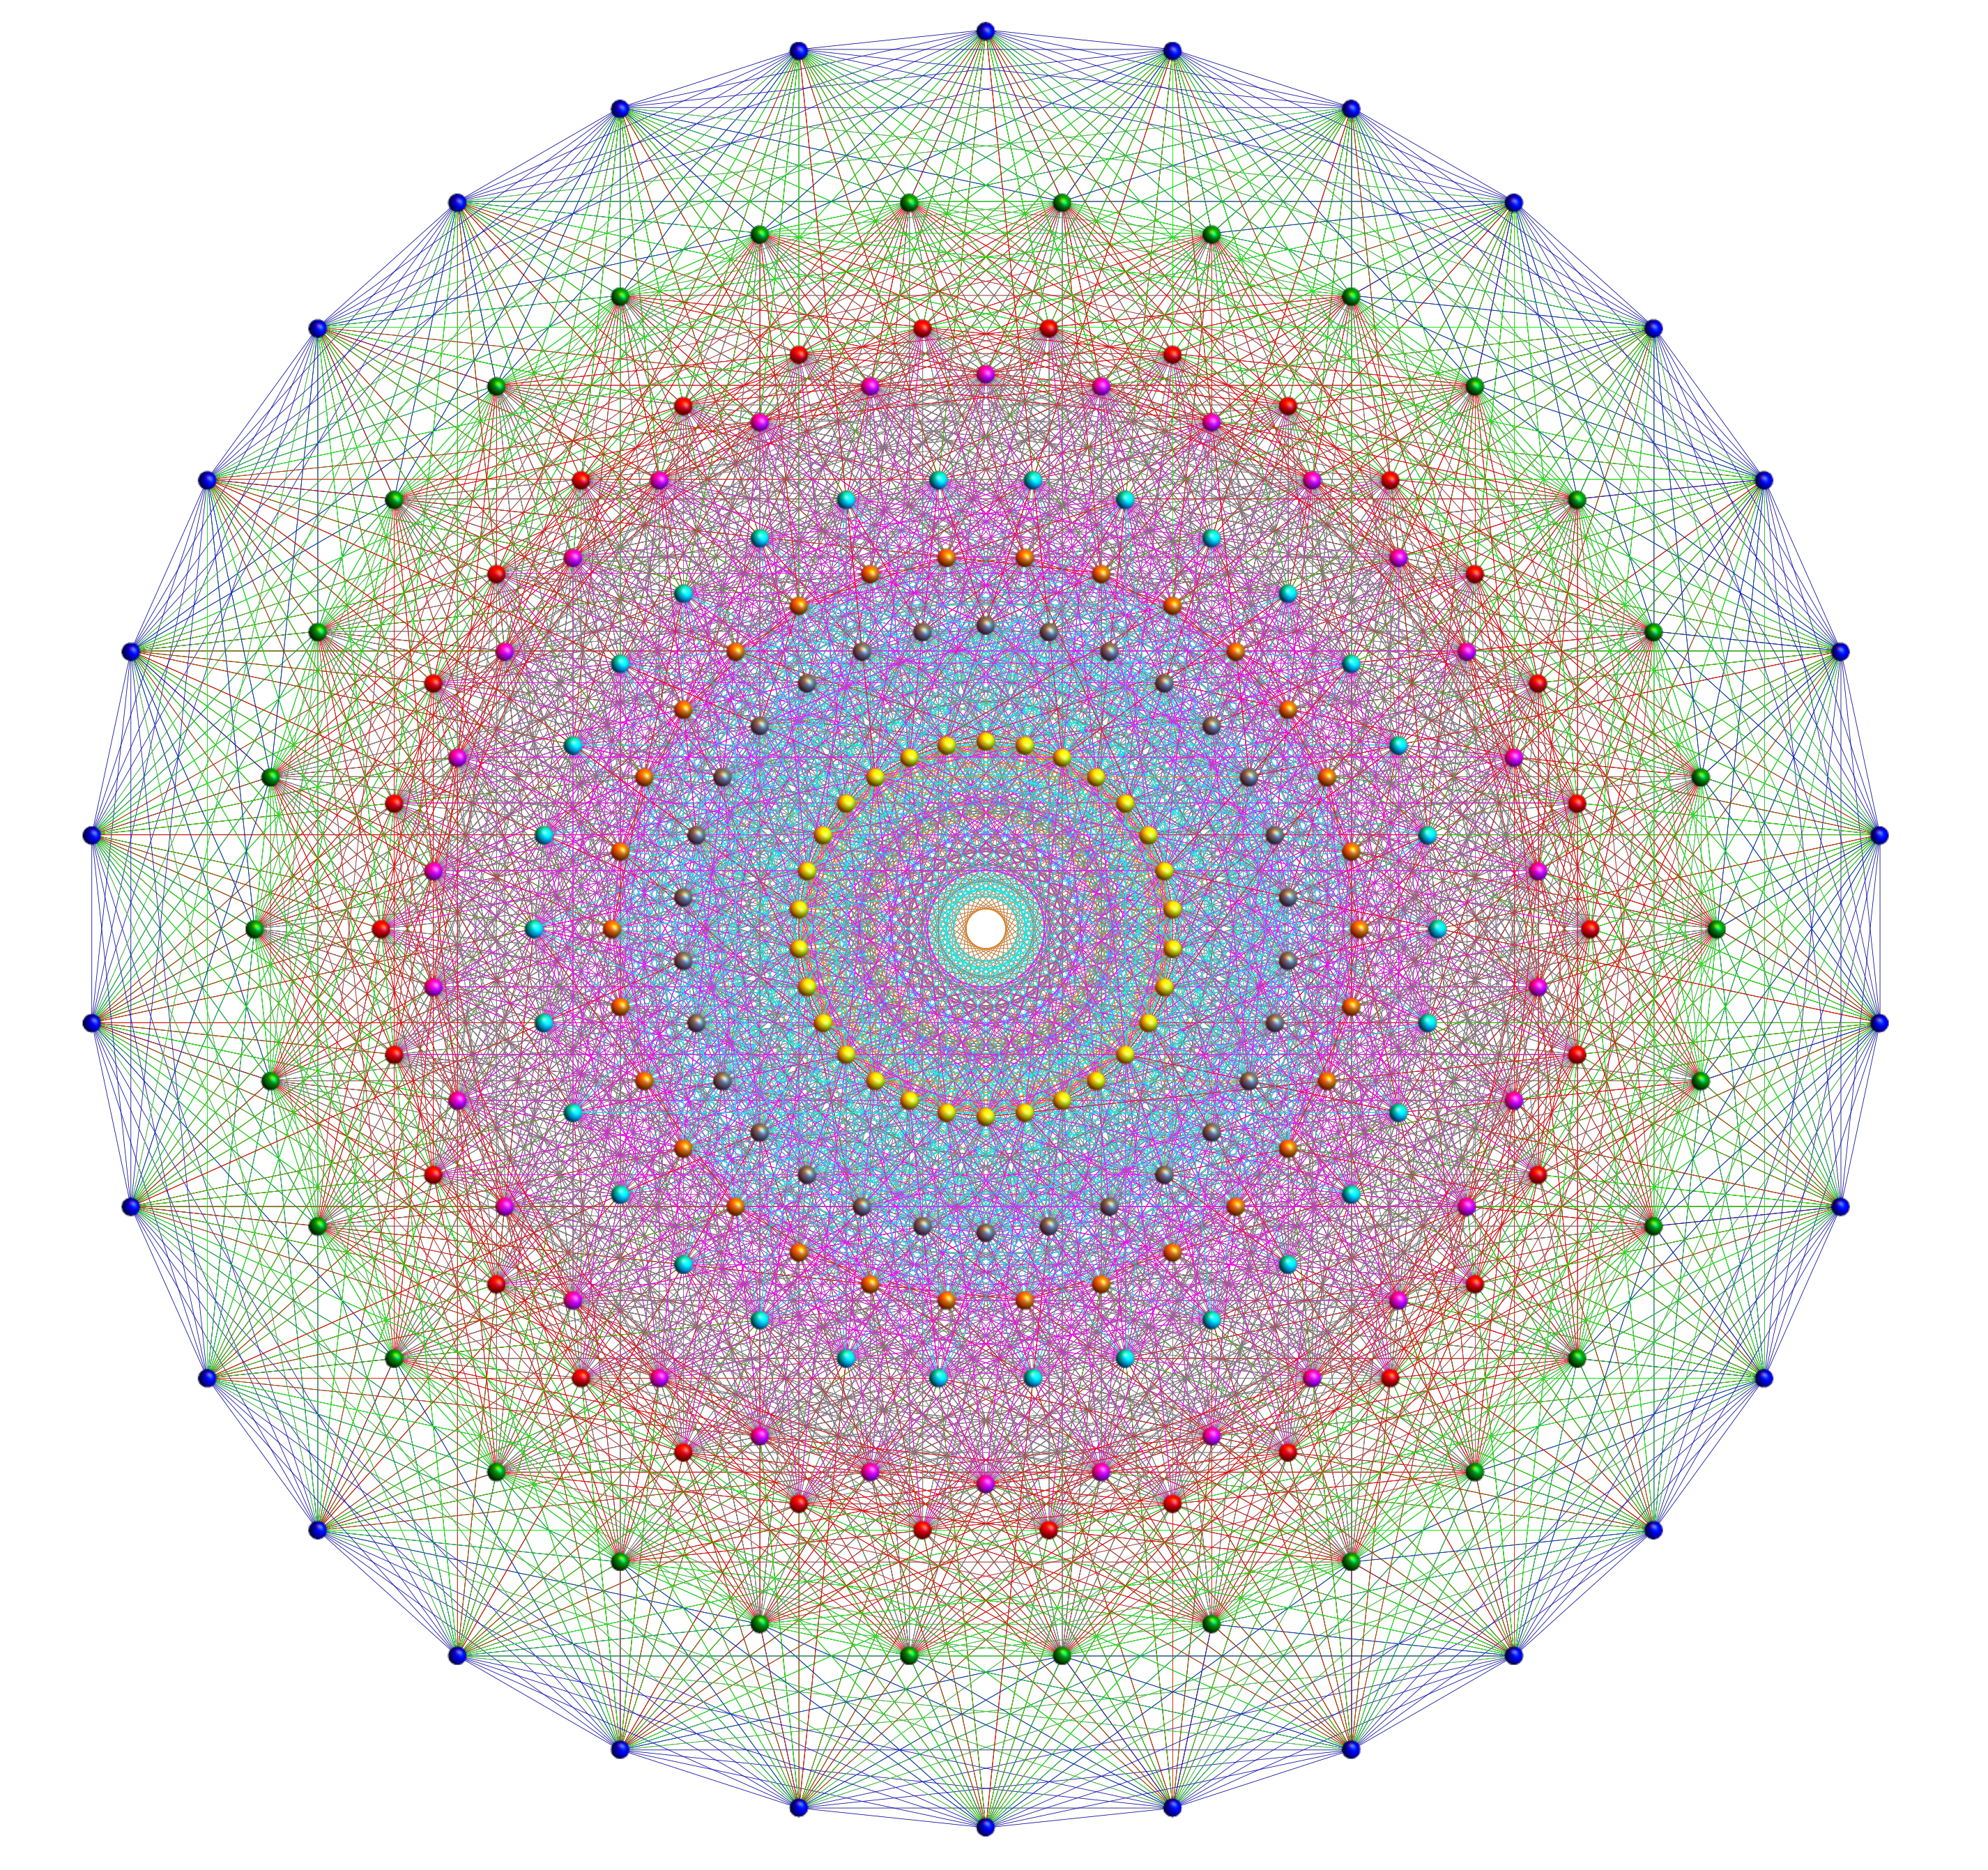
\includegraphics[width=.8\columnwidth]{front.png}
\end{figure}
\newpage
\tableofcontents 
\newpage
\section{Gli interi}
\subsection{Propriet\`a di base}
Una propriet\`a dei numeri interi, che si prender\`a come assiomatica, \`e quella del \textit{buon ordinamento}: 
\begin{center}
	\textit{Ogni insieme non-vuoto di interi maggiori o uguali a $0$, ha un elemento minimo.}
\end{center}
Da questa deriva la seguente.
\begin{teorema}
	{Principio di induzione (prima forma)}{}
	Sia $A(n)$ un'affermazione valida per ogni intero $n\ge 1$. Se
	\begin{enumerate}[(1).]
		\item $A(1)$ \`e vera,
		\item $\forall n \ge  1$, se $A(n)$ \`e vera $\implies A(n+1)$ \`e vera,
	\end{enumerate}
	allora, $\forall n \ge  1$, $A(n)$ \`e vera.
	\begin{proof}
		Sia $S $ l'insieme di interi per cui $A(n)$ \`e falsa. Si mostra che $S$ \`e l'insieme vuoto. 
		Si assume per assurdo che $S\neq \varnothing\Rightarrow \exists n_0 \in S$, con $n_0$ minimo (esistente per il buon ordinamento), e, per assunzione, deve essere $n_0 \neq 1 \Rightarrow  n_0>1$. 
		Questo vuol dire che $n_0 -1$ non \`e in $S$ e, quindi, $A(n_0-1)$ \`e vera.

		Per la propriet\`a (2), per\`o, deve essere vera anche $A(n_0)$ perch\'e $n_0 = (n_0-1) + 1$, il che \`e assurdo e, pertanto, $S = \varnothing$.
	\end{proof}
\end{teorema}

\begin{obs}
	Nella dimostrazione sopra, si sarebbe potuto sostituire $1$ con $0$ e far partire il principio di induzione da $n=0$ piuttosto che da $n=1$ e non sarebbe cambiato nulla.
\end{obs}
\noindent Il principio di induzione pu\`o essere espresso in una forma alternativa, come segue.
\begin{teorema}
	{Principio di induzione (seconda forma)}{}
	Sia $A(n)$ affermazione vera $\forall n\ge 0$ e sia possibile mostrare che:
	\begin{enumerate}[(1').]
		\item $A(0)$ \`e vera;
		\item $\forall n > 0$, se $A(k)$ \`e vera $\forall 0\le k < n$, allora $A(n)$ \`e vera.
	\end{enumerate}
	Allora $A(n)$ \`e vera $\forall n\ge 0$.
	\begin{proof}
	Sia ancora $S$ l'insieme degli interi che non soddisfano $A(n)$. 
	Ancora per assurdo, si prende $S\neq \varnothing$, quindi deve esistere, per il buon ordinamento, un $n_0 \in S$ minimo.

	Per punto (1'), deve valere $n_0 \neq 0$ e, visto che $n_0$ \`e minimo, $\forall k$ intero tale che $0\le k< n_0$, $A(k)$ deve essere vera. 
	Per il punto (2'), per\`o, deve essere vera anche $A(n_0)$, arrivando nuovamente all'assurdo.
	\end{proof}
\end{teorema}
\noindent Un altro importante risultato del buon ordinamento \`e l'\textit{algoritmo di Euclide}.
\begin{teorema}
	{Algoritmo di Euclide}{}
	Siano $m,n$ interi, con $m>0$; allora esistono interi $q,r$, con $0\le r< m$, tali che
	\begin{equation}
		n = qm  + r
	\end{equation}
	Inoltre, gli interi $q,r$ sono univocamente determinati da tali condizioni.
	\begin{proof}
		Visto che l'insieme degli interi $q$ tali per cui $qm\le n$ \`e limitato superiormente per definizione, si pu\`o usare il buon ordinamento per affermare che esiste un elemento pi\`u grande\footnote{Basta applicare il buon ordinamento all'elemento pi\`u piccolo dell'insieme $n-qm$.} tale che
		\[
		qm \le n < (q+1) m = q m + m
		\] 
		ossia $0\le n - qm < m$. Sia $r = n - qm$, per cui vale $0\le r < m$. Questo dimostra l'esistenza di $r,q$ come descritti.

		Per l'unicit\`a, si assume che valga contemporaneamente
		\[
		\begin{cases}
			n = q_1m + r_1&, \ 0\le r_1<m\\
			n = q_2m + r_2&, \ 0\le r_2<m\\
		\end{cases}
		\] 
		con $r_1 \neq r_2$. Sia, per esempio, $r_2> r_1$; allora, sottraendo le due, si ha $(q_1-q_2) m = r_2-r_1$. 
		Per\`o, si ha $r_2-r_1> 0$ e $r_2-r_1 < m$, il che non \`e possibile perch\'e $q_1-q_2$ \`e un intero per cui $(q_1 - q_2)m > 0$, quindi si avrebbe $r_2-r_1 = (q_1-q_2)m \ge m$ e, quindi $r_2-r_1\ge m$.
		Pertanto, deve essere $r_1=r_2$, che fra l'altro implica $q_1m=q_2m$, per cui $q_1=q_2$.
	\end{proof}
\end{teorema}
\noindent Da questo teorema, si definisce $r$ come il \textit{resto della divisione di $n$ per $m$}.
\subsection{Massimo comune divisore}
Siano $n, d$ due interi diversi da $0$.
Si dice che $d$ \textit{divide} $n$ se esiste $q$ intero tale che $n = dq$; in questo caso, si scrive $d|n$.
Se $m,n$ sono interi non-nulli, per \textit{divisore comune} di $m$ e $n$ si intende un intero $d\neq 0$ tale che $d | m$ e $d | n$. 
Allora si ha la seguente definizione.
\begin{definizione}
	{Massimo comune divisore}{}
	Per massimo comune divisore di $m,n$ interi non nulli, si intende un intero $d>0$, divisore comune di $m$ e $n$, e tale che $\forall e $ intero positivo che divide $m$ e $n$, si ha anche $e|d$.
\end{definizione}
\noindent Chiaramente, il massimo comune divisore \`e univocamente determinato e si mostrer\`a che esiste sempre. 
Per farlo, si d\`a prima la seguente definizione.
\begin{definizione}
	{Ideale}{}
	Sia $J\subseteq \mathbb{Z}$ un sottoinsieme degli interi. Si dice che $J$ \`e un \textit{ideale} se:
	\begin{itemize}
		\item $0 \in J$;
		\item $m,n\in J\implies m+n \in J$
		\item se $m\in J$ e $n$ \`e un intero qualsiasi, allora $mn \in J$.
	\end{itemize}
\end{definizione}
\begin{obs}
	Di seguito, per ideale si intender\`a sempre un sottoinsieme degli interi.
\end{obs}
\noindent Siano $m_1, \ldots,m_r$ interi. Sia $J$ l'insieme di tutti gli interi che si scrivono come
\[
x_1m_1+\ldots+x_r m_r
\] 
con $x_1,\ldots,x_r$ interi. 
Allora \`e automaticamente verificato che $J$ \`e un ideale. Infatti
\begin{itemize}
	\item se $y_1,\ldots,y_r$ sono interi, allora
		\[
		\sum_{i=1}^{r} x_i m_i +  \sum_{j=1}^{r} y_j m_j = (x_1 + y_1) m_1 + \ldots + (x_r + y_r) m_r
		\] 
		che, quindi, appartiene a $J$;
	\item se $n$ \`e un intero, si ha
		\[
		n \sum_{i=1}^{r} x_i m_i = nx_1m_1 + \ldots+ nx_r m_r
		\] 
		che, quindi, appartiene a $J$;
	\item si pu\`o scrivere $0$ come $0m_1 + \ldots + 0m_r$, quindi anche $0 \in J$.
\end{itemize}
In questo caso, si dice che $J$ \`e \textbf{generato} dagli interi $m_1,\ldots,m_r$ e che questi sono i suoi \textbf{generatori}. L'insieme $\left\{ 0 \right\} $ \`e esso stesso un ideale, chiamato \textbf{ideale nullo}. 
Inoltre, $\mathbb{Z}$ \`e detto \textbf{ideale unit\`a}.
Ora si pu\`o dimostrare il seguente.
\begin{teorema}
	{}{smalld}
	Sia $J$ un ideale di $\mathbb{Z}$. Allora esiste un intero $d$ che \`e un generatore di $J$. Inoltre, se $J \neq \left\{ 0 \right\} $, allora $d$ \`e il pi\`u piccolo intero positivo in $J$.
	\begin{proof}
	Sia $J$ l'ideale nullo; allora $0$ \`e un suo generatore.
	Sia, ora, $J \neq \left\{ 0 \right\} $; se $n \in J$, allora $-n = (-1) n $ \`e anche in $J$, quindi $J$ contiene degli interi positivi.
	Si vuole dimostrare che $d$, definito come il pi\`u piccolo intero positivo, \`e un generatore.
	Per farlo, sia $n \in J$, con $n = dq + r, \ 0\le  r < d$; allora $r = n - dq \in J$ e, visto che vale $r < d$, segue che $r = 0$\footnote{Altrimenti $d$ non sarebbe il pi\`u piccolo intero positivo.}, quindi $n = dq$ e, allora, $d$ \`e un generatore.
	\end{proof}
\end{teorema}
\begin{teorema}
	{}{bezid}
	Siano $m_1,m_2$ due interi positivi e sia $d$ un generatore positivo per l'ideale generato da $m_1,m_2$. Allora $d$ \`e il massimo comune divisore di $m_1,m_2$.
	\begin{proof}
		Per definizione, $m_1,m_2 \in J$\footnote{Questo \`e ovvio perch\'e $m_1 = 1m_1 + 0 m_2$ e $m_2  = 0 m_1 + 1 m_2$.}, quindi esiste un intero $q_1$ tale che $m_1=q_1 d$, per cui $d|
		m_1$.
		Analogamente $d|m_2$.
		Sia, poi, $e$ un intero non-nullo che divide sia $m_1$ che $m_2$ come $m_1 = h_1 e$ e $mm_2=h_2 e$, con interi $h_1,h_2$.
		Visto che $d$ \`e nell'ideale generato da $m_1,m_2$, esistono degli interi $s_1,s_2$ tali che $d = s_1m_1 + s_2m_2$, quindi
		\[
		d = s_1h_1e + s_2h_2e = (s_1h_1 + s_2h_2) e
		\] 
		Quindi $e $ divide $d$ e il teorema \`e dimostrato.
	\end{proof}
\end{teorema}
\begin{obs}
	La stessa esatta dimostrazione funziona per pi\`u di due interi, quindi se si considerassero $m_1,\ldots,m _r$ degli interi, con $d$ generatore positivo dell'ideale da loro generato, $d$ sarebbe anche il massimo comune divisore.
\end{obs}
\noindent Questi due teoremi permettono di concludere i seguenti fatti.
\begin{itemize}
	\item Ogni ideale $J$ contiene un numero intero che lo genera interamente e questo coincide col pi\`u piccolo intero positivo in esso contenuto, quindi \`e l'unico generatore \textit{singolo} dell'ideale.
	\item Ogni insieme di numeri interi ha un massimo comune divisore perch\'e tale insieme genera un ideale, il quale, per\`o, contiene un generatore (pi\`u piccolo numero intero in esso contenuto) che \`e un massimo comune divisore per l'insieme di interi iniziale.
\end{itemize}
\begin{definizione}
	{Interi coprimi}{relprime}
	Siano $m_1,\ldots,m_r$ degli interi il cui massimo comune divisore \`e $1$. 
	Allora $m_1,\ldots,m_r$ si dicono \textit{coprimi} e, per questi, esistono interi $x_1,\ldots,x_r$ tali che
	\[
	x_1m_1   +\ldots + x_r m_r = 1
	\] 
	perch\'e $1$ appartiene all'ideale generato dagli $m_i$.
\end{definizione}
\`E immediato verificare per definizione di ideale che $1 \in  J \iff J \equiv \mathbb{Z}$.
Dalla definizione \ref{def:relprime} segue direttamente che ogni insieme di interi coprimi genera $\mathbb{Z}$.
\begin{obs}
	Si potrebbe pensare che se $p$ \`e un numero primo, allora l'insieme $\left\{ p \right\} $ generi $\mathbb{Z}$, cio\`e $p$ generi $\mathbb{Z}$. 
	Questo \`e ovviamente falso sia perch\'e, evidentemente, $J_p$ non contiene $1$, sia perch\'e $p$ non \`e coprimo con se stesso, avendo come altro divisore proprio $p$ oltre che $1$.
\end{obs}
\subsection{Fattorizzazione unica}
\begin{definizione}
	{Numero primo}{}
	Si dice che $p$ \`e un numero primo se \`e un intero e $p\ge   2$ tale che, data una fattorizzazione $p = mn $, con interi positivi $m,n$, allora $m=1$ o $n=1$.
\end{definizione}
\begin{obs}
	Il fatto che $p=mn$ con $m=1$, o $n=1$ implica $p$ numero primo significa che $p$ \`e diviso unicamente o da $1$ o, da se stesso.
\end{obs}
\noindent Ora si mostra che ogni numero intero ammette un'unica scomposizione in numeri primi. 
Per dimostrare l'unicit\`a di tale scomposizione, si introduce il seguente lemma.
\begin{lemma}
	{}{lemmaprimdecomp}
	Sia $p$ un numero primo e siano $m,n$ interi non-nulli e tali che $p$ divide $mn$. Allora o $p|m$ o $p |n$.
	\begin{proof}
		Senza perdita di generalit\`a, si assume che $p$ \textit{non} divida $m$. 
		Allora, il massimo comune divisore di $p$ e $m$ deve essere $1$, pertanto esistono interi $a,b$ tali per cui $1 = ap + bm$.

		Ora, moltiplicando ambo i membri per $n$, si ha $n = nap + bmn$, ma $mn = pc$ per qualche intero $c$ (essendo in assunzione $mn$ divisibile per $p$), quindi
		\[
		n = nap + bpc = (na + bc) p
		\] 
		il che implica che $p$ divide $n$.
	\end{proof}
\end{lemma}
\noindent Per evidenziare l'utilit\`a del lemma nel seguente teorema, si nota che se $p$ divide un prodotto di numeri primi $q_1\ldots q_s$, si hanno due possibilit\`a: o $p$ divide $q_1$, o divide $q_2 \ldots q_s$; se divide $q_1$, allora $p \equiv q_1$, altrimenti si trova $p\equiv q_i$ procedendo induttivamente. 
Il caso interessante \`e quando si ha un uguaglianza tra prodotti di numeri primi 
\[
p_1 \ldots p_r = q_1\ldots q_s
\] 
dove ogni $p_i$ divide il prodotto\footnote{Per vederlo, \`e sufficiente prendere $c = p_1 \ldots p_{i-1} p_{i+1} \ldots p_r$, quindi si ha $c p_i = q_1 \ldots q_s$, che \`e la definizione di $p_i | q_1 \ldots q_s$.}. Rinumerandoli, si pu\`o assumere senza perdita di generalit\`a che $p_1 = q_1$ e, induttivamente, che $p_i = q_i$ e $r = s$, essendo due scomposizioni in un numeri primi.
\begin{teorema}
	{}{}
	Ogni intero positivo $n\ge   2$ ammette una fattorizzazione come prodotto di numeri primi (non necessariamente distinti) $n=p_1\ldots p_r$ e tale fattorizzazione \`e unica.
	\begin{proof}
		Si assume per assurdo che esista almeno un intero $\ge  2 $ che non possa essere espresso come prodotto di numeri primi.
		Sia $m$ il pi\`u piccolo di questi. 

		Per costruzione, $m$ non pu\`o essere primo, quindi $m = de$, con $d,e > 1$. 
		Visto che $d$ ed $e$ sono minori di $m$ e visto che $m$ \`e scelto per essere il pi\`u piccolo fra gli interi non fattorizzabili come numeri primi, allora sia $d$ che $e$ ammettono scomposizione in prodotto di numeri primi:
		\[
		\begin{split}
			&d = p_1 \ldots p_r \\
			&e = p'_1 \ldots p'_s
		\end{split}\implies m = p_1 \ldots p_r p'_1 \ldots p'_s
		\] 
	da cui l'assurdo.	

	Per mostrare l'unicit\`a, si usa il lemma \ref{lem:lemmaprimdecomp}. 
	Come conseguenza, diretta del lemma, se esistessero due scomposizioni in primi $p_1 \ldots p_r $ e $p'_1 \ldots p'_s$, varrebbe $p_1 \ldots p_r = p'_1 \ldots p'_s\Rightarrow p_i = p'_i$ e $r = s$, da cui l'unicit\`a
	\end{proof}
\end{teorema}
\subsection{Identit\`a di B\'ezout e equazioni diofantee}

\subsubsection{Identit\`a di B\'ezout}
L'identit\`a di B\'ezout non \`e altro che quanto espresso in teorema \ref{th:bezid}. Di seguito lo si enuncia senza ricorrere a tale trattazione. 
\begin{teorema}
	{Identit\`a di B\'ezout}{}
	Dati $a,b \in \mathbb{Z}$ non entrambi nulli, esistono altri due interi $m,n$ tali che:
	\[
	\operatorname{gcd} (a,b) = am +  bn
	\] 
\begin{proof}
	Si considera l'insieme di tutte le possibili combinazioni lineari positive di $a,b$, dato da $\mathrm{CL} ^+(a,b) : = \left\{ ar+ bs : r, s \in \mathbb{Z} , \ ar + bs > 0 \right\} $. Questo \`e non-vuoto perch\'e, assumendo senza perdita di generalit\`a $a\neq 0$, esistono, per $s =0 $, degli $r\in \mathbb{Z}$ tali che $ra >0 $.

	Visto che $\mathrm{CL} ^+(a,b) \subseteq \mathbb{N}$, per il principio del buon ordinamento, questo ammette un minimo $d$; in quanto tale $\exists m,n \in \mathbb{Z}:d = am + bn$. 
	Infine, si motra che $d = \operatorname{gcd} (a,b)$, cio\`e si mostrano i seguenti punti.
	\begin{itemize}
		\item Si ha $d|a$ e $d|b$.

			Dividendo $a$ per $d$, si ha $a = qd +r$, con $0\le r < d$, quindi
			\[
			a = q ( am +  bn) + r
			\] 
			da cui 
			\[
			r = (-qm + 1) a + (-qn) b
			\] 
			In questo modo, $r$ \`e combinazione lineare di $a,b$ ed \`e minore di $d$, ma questo \`e assurdo perch\'e $d $ era minimo per assunzione, quindi deve essere $r= 0$. Allo stesso modo si mostra $d | b$.
		\item Se $c|a$ e $c|b \implies c \le d$.

			Questo \`e vero perch\'e se $c|a, \ c|b$, allora (in particolare) $c | (am + bn) $, cio\`e $ c | d \Rightarrow c\le d$.
	\end{itemize}
\end{proof}
\end{teorema}
\begin{obs}
	Il teorema afferma l'esistenza di una possibile coppia $(m,n) \in \mathbb{Z} \times \mathbb{Z}$ che soddisfa $\operatorname{gcd} (a,b) = am + bn$, ma non ne specifica l'unicit\`a; di fatto, si vedr\`a che di coppie simili ce ne sono infinite.
\end{obs}
\begin{corollario}
	{}{}
	Dati $a,b \in \mathbb{Z}$ non entrambi nulli e sia $c\in \mathbb{Z} : c|a$ e $c|b$; allora $c | \operatorname{gcd}(a,b) $. 
\end{corollario}
Complessivamente, esattamente come riportato nel teorema \ref{th:bezid}, si \`e dimostrato che il massimo comune divisore di due interi $a,b$ \`e la pi\`u piccola combinazione lineare positiva ottenibile dai due.
\begin{corollario}
	{}{c1}
	Dati $a,b$ non entrambi nulli e $\operatorname{gcd}(a,b) $ il loro massimo comune divsore, allora gli interi 
	\[
		a' = \frac{a}{\operatorname{gcd}(a,b) } \hspace{2cm} b' = \frac{b}{\operatorname{gcd}(a,b) }
	\] 
	sono coprimi.
	\begin{proof}
	Si pu\`o dimostrare in due modi diversi. Nel primo, si assume per assurdo che esista un divisore comune $d> 1 $ di $a' , b'$; se cos\`i fosse, per\`o, $d \cdot \operatorname{gcd}(a,b) $ dividerebbe sia $a$ che $b$ e sarebbe pi\`u grande di $\operatorname{gcd}(a,b) $ stesso, il che \`e assurdo.

	Il secondo fa uso dell'identit\`a di B\'ezout per cui $\operatorname{gcd}(a,b) = am+bn $; dividendo per $\operatorname{gcd}(a,b) $, si ha:
	\[
	1 = a'm + b'n 
	\] 
	per cui $1$ \`e il pi\`u piccolo intero positivo  ottenibile come combinazione lineare positiva di $a', b'$, quindi i due sono coprimi.
	\end{proof}
\end{corollario}
\begin{teorema}
	{}{d1}
	Siano $a,b,c \in \mathbb{Z}$; se $a|bc$ e $\operatorname{gcd}(a,b) =1$, allora $a|c$.
	\begin{proof}
		Per B\'ezout, visto che $\operatorname{gcd}(a,b) = 1$, si ha $1 = an + bm$ per una coppia di numeri $m,n \in \mathbb{Z}$. 
		Moltiplicando ambo i membri per $c$, ne segue che:
		\[
		c = acn + bcm
		\] 
		quindi $a | c$ perch\'e, ovviamente, $a | acn$, mentre $a | bcm$ perch\'e, per ipotesi, $a | bc$, quindi $a| (acn + bcm)$, cio\`e $a | c$.
	\end{proof}
\end{teorema}
\noindent Il teorema appena dimostrato \`e alla base del fatto che la fattorizzazione di interi in numeri primi \`e unica.

\subsubsection{Equazioni diofantee}


Dati $a,b,c \in \mathbb{Z}$, si dice \textbf{equazione diofantea} un'equazione del tipo	
\begin{equation}
	ax + by = c
\end{equation}
La sua soluzione \`e una coppia di interi $(\overline{x},\overline{y}) \in \mathbb{Z} \times \mathbb{Z}$ che la soddisfa.

\begin{obs}
	L'equazione diofantea con $a=b=0$ ha soluzione $\iff c= 0$ e ne ammette infinite, consistenti in tutte le possibili coppie $(\overline{x},\overline{y}) \in \mathbb{Z}\times \mathbb{Z}$, perch\'e ogni coppia soddisfa $0 x + 0y = c$.
\end{obs}
Per il caso generale di $a,b$ non entrambi nulli, si ha il seguente.
\begin{teorema}
	{}{solco}
	L'equazione $ax + by = c$, con $a,b$ non entrambi nulli, ha soluzione $\iff \operatorname{gcd} (a,b )  | c$.
	\begin{proof}
		Per l'identit\`a di B\'ezout, si sa che vi \`e soluzione all'equazione 
		\[
		ax + by = \operatorname{gcd}(a,b) 
		\] 
		L'equazione da risolvere \`e diversa: al posto di $\operatorname{gcd}(a,b) $ c'\`e $c$; allora la dimostrazione si basa sul capire se $\operatorname{gcd}(a,b) $ divide o meno $c$.

		Nel caso in cui $\operatorname{gcd}(a,b) | c$ (per cui si ha $c = k\cdot \operatorname{gcd}(a,b) $ per qualche intero $k$), allora l'equazione diofantea ammette soluzione. Infatti, dopo aver trovato $(m,n) \in \mathbb{Z} \times \mathbb{Z}$ che risolve $am + bn = \operatorname{gcd}(a,b) $, si ha che $(m k , nk) \in \mathbb{Z} \times \mathbb{Z}$ risolve l'equazione diofantea perch\'e 
		\[
		k \cdot (am + bn ) = akm + bkn = k\cdot \operatorname{gcd}(a,b) = c
		\] 
		Viceversa, se $\operatorname{gcd}(a,b)$ non divide $c$, allora non vi \`e soluzione. Se, per assurdo, vi fosse soluzione, sia questa $(\overline{x},\overline{y})$, allora $a \overline{x}+ b \overline{y}=c$ implica che $\operatorname{gcd}(a,b) | c$ perch\'e $\operatorname{gcd}(a,b) $ divide il membro di sinistra (essendo un divisore sia di $a$ che di $b$). 
		Questo, per\`o, \`e assurdo perch\'e si era nell'ipotesi in cui $\operatorname{gcd}(a,b) \not | \ c$.
	\end{proof}
\end{teorema}
Si considera il caso in cui l'equazione $ax + by = c$ ha soluzione; si vuole capire se la soluzione \`e unica, o se ve ne sono di pi\`u. 
Si considera, a tal proposito, l'\textbf{omogenea associata} $ax + by = 0$. 
\begin{obs}
	La comodit\`a nel lavorare con l'omogenea associata sta nel fatto che se $(\overline{x}, \overline{y})$ risolve $ax + by = c$ e  $(\gamma, \delta )$ risolve l'omogenea, allora $(\overline{x}+\gamma, \overline{y}+\delta )$ \`e ancora soluzione di $ax + by = c$.
\end{obs}
\noindent L'obiettivo, ora, \`e di trovare il numero delle soluzioni per l'omogenea associata.
Si nota che $ax + by =0 \Rightarrow  axa = - by$; si risolve
\[
\frac{a}{\operatorname{gcd}(a,b) } x = - \frac{b}{\operatorname{gcd}(a,b) } y 
\] 
Sia $(\gamma, \delta )$ una soluzione di questa; visto che $a/\operatorname{gcd}(a,b) $ e $b / \operatorname{gcd}(a,b) $ sono coprimi\footnote{Vedi corollario \ref{cor:c1}.}, il teorema \ref{th:d1} afferma che $a / \operatorname{gcd}(a,b) $ divide $\delta $, quindi $\delta $ \`e della forma $\frac{a}{\operatorname{gcd}(a,b)}  t$ e $\gamma$, analogamente, \`e della forma $- \frac{b}{\operatorname{gcd}(a,b)} t$.

Al contrario, si nota facilmente che una qualunque coppia della forma $\left( - \frac{b}{\operatorname{gcd}(a,b) }t , \frac{a}{\operatorname{gcd}(a,b) }t\right)$, con $ t \in \mathbb{Z} $ \`e una soluzione dell'omogenea associata. 
Questo significa che le soluzioni dell'omogenea associata sono tutte di questa forma, pertanto sono infinite.

Da questo discorso, si pu\`o concludere che anche le soluzioni dell'equazione diofantea iniziale $ax + by = c$ sono infinite. 
Il teorema di seguito permette di concludere, ulteriormente, che \textit{tutte} le soluzioni di $ax + by = c$ sono esprimibili tramite quelle dell'omogenea, quindi equazione originale e omogenea hanno lo stesso numero di soluzioni.
\begin{teorema}
	{}{}
	Se l'equazione $ax + by = c$ ammette soluzione, allora ne ammette infinite. Data $(\overline{x}, \overline{y})$ una sua soluzione, l'insieme $\mathcal{S} $ di tutte le soluzioni di $ax +by = c$ \`e ottenibile come
	\[
	\mathcal{S}  = \left\{ (\overline{x}+\gamma, \overline{y}+\delta ) : (\gamma, \delta ) \text{ soluzione dell'omogenea associata}\right\} 
	\] 
	\begin{proof}
		Per quanto detto sopra, si conclude che 
		\[
		\left\{(\overline{x}+\gamma, \overline{y}+\delta ) : (\gamma, \delta ) \text{ soluzione dell'omogenea associata}  \right\} \subseteq \mathcal{S} 
		\] 
		Si deve mostrare l'inclusione inversa.
		Questo segue direttamente dal fatto che, se $(\alpha ,\beta )$ \`e soluzione di $ax + by = c$, allora $(\alpha -\overline{x}, \beta - \overline{y})$ \`e soluzione dell'omogenea associata.
	\end{proof}
\end{teorema}



\subsection{Relazioni di equivalenza e congruenza}
\begin{definizione}
	{Relazione di equivalenza}{}
	Sia $S$ un insieme.
	Una relazione di equivalenza su $S$ \`e una relazione indicata con $x \sim y, \ x, y \in S$, tale che:
	\begin{enumerate}[ER 1.]
		\item $\forall x \in S, \ x \sim x$;
		\item se $x \sim y$ e $y\sim z$, allora $x \sim z$;
		\item se $x\sim y$, allora $y \sim x$.
	\end{enumerate}
\end{definizione}
\noindent Se su $S$ \`e definita una relazione di equivalenza $\sim$, le classi di equivalenza sono insiemi $C_x : = \left\{ y \in S : y \sim x \right\} $ partizionano $S$ in insiemi disgiunti. 
Inoltre, dati due elementi $r,s \in S$, si ha $C_r \equiv C_s$, oppure $C_r,\ C_s$ non hanno elementi in comune.
Si sceglie un elemento che identifica la classe di equivalenza, ad esempio $x$ per $C_x$, e tale elemento si chiama rappresentante della classe di equivalenza. 
Un esempio di relazione di equivalenza \`e la congruenza.
\begin{definizione}
	{Congruenza}{}
	Sia $m \in \mathbb{Z}^+$ e $a,b \in \mathbb{Z}$; si dice che $a$ \`e \textit{congruente} $b$ \textit{modulo} $m$ se $\exists k \in \mathbb{Z} : a-b = km$. In tal caso, si scriver\`a $a \equiv b  \pmod{m}  $.
\end{definizione}
\begin{obs}
	La definizione pi\`u esplicativa di congruenza \`e che due numeri $a,b \in \mathbb{Z}$ di dicono congruenti modulo $m \in \mathbb{Z}^+$ se, divisi per $m$, restituiscono lo stesso resto.
	Di fatto, da questa discende la definizione data sopra: se $a = qm + r, \ b = pm + r \Rightarrow a - b = (q-p)m$.
\end{obs}
\begin{definizione}
	{Interi pari e dispari}{}
Si definiscono gli interi \textbf{pari} come quelli che sono congruenti a $0 \pmod{2} $ (quindi $n = 2m$) e quelli \textbf{dispari} come gli interi che non sono pari, quindi della forma $2m + 1$, per qualche intero $m$.
\end{definizione}
\noindent Dalla definizione di congruenza, si ha che $a\equiv b \pmod{m}  \Rightarrow  a- b = qm$, quindi $a-b$ appartiene all'ideale generato da $m$.

Inoltre, la stessa relazione implica che $m | (a-b)$; viceversa, se $a \not \equiv b \pmod{m} $, allora i due numeri divisi per $m$ avrebbero resti diversi: $a = k_1 m + r_a, \ b = k_2 m + r_b$, il che implica che $a-b = (k_1 - k_2)m + (r_a- r_b)$, che non \`e divisibile per $m$; allora is ha il seguente.
\begin{prop}
	{}{}
	Siano $m \in \mathbb{Z}^+$ e $a,b \in \mathbb{Z}$; $a$ e $b$ sono congruenti se e soltanto se $m | (a-b)$.
\end{prop}
\begin{prop}
	{Addizione e moltiplicazione in congruenza}{}
	Dati $a\equiv a' \pmod{m} $ e $b\equiv b' \pmod{m} $, si ha:
	\[
		\begin{split}
			&a + b \equiv a' + b' \pmod{m}  \\
			& a b\equiv a'b' \pmod{m} 
		\end{split}
	\] 
\begin{proof}
	Per definizione, si ha $a ' = a + km$ e $b' = b + k'm $; quindi:
	\[
	a' + b ' = a+ b + (k+k') m\implies a' + b' \equiv a + b\pmod{m} 
	\] 
	Per la moltiplicazione, si nota che 
	\[
	a' b ' = a b + m(kb + k'a) +kk'm^2
	\] 
	da cui si vede che $a'b' - ab$ \`e divisibile per $m$, quindi $a'b' \equiv ab \pmod{m} $.
\end{proof}	
\end{prop}
La divisione in congruenza funziona diversamente; infatti $2 \cdot  7 \equiv 2 \cdot  4 \pmod{6} $, ma $7 \not \equiv 4 \pmod{6} $. 
Si ha il seguente.
\begin{teorema}
	{Divisione in congruenza}{}
	Sia $m \in \mathbb{Z}^+$; $\forall a \in  \mathbb{Z} \setminus \left\{ 0 \right\} $ e dati $b_1,b_2 \in \mathbb{Z}$, vale
	\[
	ab_1 \equiv ab_2 \pmod{m} \iff b_1 \equiv b_2 \mod{\frac{m}{\operatorname{gcd}(a,m) }} 
	\] 
	Questo vuol dire che la divisione \`e ammessa a patto di dividere il modulo per $\operatorname{gcd}(a,m) $.
	\begin{proof}
		Si mostra l'implicazione verso destra.
		Per definizione, $m  \mid  (ab_1- ab_2)$, quindi $\exists q \in \mathbb{Z} : mq = ab_1 - ab_2$.
		Dividendo per $\operatorname{gcd}(a,m) $:
		\[
		\frac{a}{\operatorname{gcd}(a,m) } (b_1-b_2) = \frac{m}{\operatorname{gcd}(a,m) } q
		\] 
		Ma $a / \operatorname{gcd}(a,m) $ e $m / \operatorname{gcd}(a,m) $ sono coprimi, quindi $\big(m / \operatorname{gcd}(a,m) \big)  \mid (b_1-b_2)$, il che implica che
		\[
		b_1\equiv b_2 \mod \frac{m}{\operatorname{gcd}(a,m) }
		\] 
		Per l'implicazione inversa, si assume che
		\[
		b_1\equiv b_2 \mod \frac{m}{\operatorname{gcd}(a,m) }
		\] 
		per cui $\exists t \in \mathbb{Z}$ tale che 
		\[
		t \frac{m}{\operatorname{gcd}(a,m) } = b_1-b_2 \implies tm  = (b_1-b_2) \operatorname{gcd}(a,m) 
		\] 
		quindi $m  \mid (b_1 -b_2) \operatorname{gcd}(a,m) $. 
		Usando che $\operatorname{gcd}(a,m) | a$, si ottiene che
		\[
		m | (b_1-b_2) a \implies ab_1 \equiv ab_2 \pmod{m} 
		\] 
	\end{proof}
\end{teorema}
\subsubsection{Inversi in congruenze}
Gli unici inversi moltiplicativi in $\mathbb{Z}$ sono $+1, -1$; operando con le congruenze, si riescono a trovare altri inversi moltiplicativi a patto di definire correttamente cosa vuol dire.
\begin{definizione}
	{Inverso in congruenza}{}
	Sia $m \in  \mathbb{Z}^+$; l'inverso di $a \in \mathbb{Z}$ \`e un certo $e \in \mathbb{Z}$ tale che
	\[
	e \cdot  a \equiv 1 \pmod{m} 
	\] 
\end{definizione}
\begin{esempio}
Per esempio, $2$ \`e l'inverso di $3 \operatorname{mod} 5$ perch\'e $2 \cdot 3 = 6 \equiv 1 \pmod{5} $.
\end{esempio}
\begin{obs}
	Quando un numero ammette inverso in congruenza, ne ammette infiniti; infatti, se $a$ \`e l'inverso di $n \operatorname{mod} m$, allora
	\[
	n \cdot  ( a+km ) \equiv n\cdot a + knm \equiv 1 + knm \equiv 1 \pmod{m} 
	\] 
\end{obs}
Non sempre un numero ammette un inverso moltiplicativo per qualche modulo; di seguito, \`e riportata una condizione necessaria e sufficiente per l'esistenza dell'inverso.
\begin{teorema}
	{}{}
	Un numero $a \in \mathbb{Z}$ ha inverso $\operatorname{mod} m $ se e solo se $\operatorname{gcd}(a,m) = 1$.
	\begin{proof}
		Si assume che $\operatorname{gcd}(a,m) =1 $; per B\'ezout, si ha:
		\[
		a u + m v = 1 
		\] 
		per qualche coppia $u,v \in \mathbb{Z}$. 
		Questa uguaglianza, letta modulo $m$, diventa:
		\[
		a u \equiv 1 \pmod{m} 
		\] 
		cio\`e $u$ \`e inverso di $a \operatorname{mod}m  $.

		Per l'implicazione inversa, si assume che $a$ abbia inverso moltiplicativo $u$.
		Questo implica che $au \equiv 1 \pmod{m} $, che, a sua volta, diventa:
		\[
		a u - mk =1
		\] 
		per qualche $k \in \mathbb{Z}$. 
		Questo \`e sufficiente per affermare che $\operatorname{gcd}(a,m) =1$. 
	\end{proof}
\end{teorema}

\subsubsection{Congruenze lineari in una incognita}
Si cercano le soluzioni $x$ alla congruenza $ax \equiv b \pmod{m} $. 
Si inizia col notare che se $\exists d \in \mathbb{Z}$ tale che $d | a$ e $d | m$, ma $d \not  \mid  b$ allora l'equazione non ha soluzioni.
\begin{proof}
	Se per assurdo ne avesse almeno una $\overline{x}$, allora sarebbe soddisfatta $a \overline{x} - b = q m $, per qualche $q \in \mathbb{Z}$. 
	Ma, nonostante $m$ sia divisibile per $d$, l'altro membro non risulta tale per via di $b$, il che \`e assurdo. 
\end{proof}
Da quanto appena notato, si conclude la condizione necessaria perch\'e esista almeno una soluzione, ossia $\operatorname{gcd}(a,m) | b$.
\begin{obs}
	Se $k | a,b$, allora l'equazionoe 
	\[
	\frac{a}{k} x \equiv \frac{b}{k} \mod \frac{m}{\operatorname{gcd}(k,m) }
	\] 
	\`e equivalente a $a x \equiv b \pmod{m} $, cio\`e hanno le stesse soluzioni. 
	Si nota in particolare che, se $s$ \`e un numero primo, allora l'equazione $sax \equiv sb \pmod{m} $ ha stesse soluzioni di quella di partenza.
\end{obs}
\begin{teorema}
	{}{}
	La congruenza $ax \equiv b \pmod{m} $ ha soluzione se e soltanto se $\operatorname{gcd}(a,m) | b$. 
	Inoltre, il numero totale di soluzioni \`e $\operatorname{gcd}(a,m) $: le altre si ottengono sommandogli un multiplo di $m$.
	\begin{proof}
		La prima parte si \`e gi\`a dimostrata, quindi si dimostra solo quella relativa al numero di soluzioni.
		Assumendo che effettivamente $\operatorname{gcd}(a,m) | b$, allora $\operatorname{gcd}(a,m) $ \`e il massimo divisore comune di $a,b,m$; allora, dividendo la congruenza per questo, si ha:
		\[
		a' x \equiv b ' \pmod{m'} 
		\] 
		dove 
		\[
		a' = \frac{a}{\operatorname{gcd}(a,m) }\hspace{1cm} b' = \frac{b}{\operatorname{gcd}(a,m) } \hspace{1cm} m' = \frac{m}{\operatorname{gcd}(a,m) }
		\] 
		dove $a'$ e $m'$ sono coprimi per costruzione. 
		Essendo coprimi, significa che $a'$ ha inverso moltiplicativo $\operatorname{mod}m' $; sia questo $e'$, il quale soddisfa $a' e '\equiv 1 \pmod{m'} $. 
		Si pu\`o guardare la relazione dal punto di vista per cui l'inverso moltiplicativo di $e'$ \`e $a'$ e $e' $ \`e coprimo con $m'$; in questo modo, si pu\`o moltiplicare per $e'$ senza modificare il modulo:
		\[
		e'a' x\equiv x \equiv e'b' \pmod{m'} 
		\] 
		quindi le soluzioni dell'equazione sono tutte e sole quelle della forma 
		\[
		x= e'b'+ qm' = e'b'+  \frac{q}{\operatorname{gcd}(a,m) } m
		\] 
		per qualche $q \in \mathbb{Z}$. 
		Questa forma permette di notare che esistono esattamente $\operatorname{gcd}(a,m) $ interi che risolvono questa equazione che non sono multipli di $m$.
	\end{proof}
\end{teorema}
\subsubsection{Il piccolo teorema di Fermat}
\begin{teorema}
	{Il piccolo teorema di Fermat}{}
	Sia $p \in \mathbb{Z}$ un numero primo e $a \in \mathbb{Z}$ tale che $a \not\equiv 0 \pmod{p} $, cio\`e $a $ non \`e multiplo di $p$\footnote{Questo basta per affermare che i due sono coprimi.}; allora 
	\[
	a^{p-1} \equiv 1 \pmod{p} 
	\] 
	\begin{proof}
		Per assunzione, $a\not \equiv 0 \pmod{p} $, quindi i numeri
		\[
		a, \ 2a, \ldots, (p-1) a
		\] 
		sono, a due a due, non congrui mod $p$ fra di loro; infatti, se cos\`i non fosse ed esistessero due numeri $i,j : 1\le  i<j\le p-1$ tali per cui $ia \equiv j a \pmod{p} $, allora $(i-j) a = q p$ per $q \in \mathbb{Z}$. 
		Questo significa che, essendo $a $ e $p$ coprimi, per cui $a$ ha inverso moltiplicativo $b$: $iab \equiv jab \pmod{m} \Rightarrow i \equiv j \pmod{m} $; questo non \`e possibile perch\'e $i$ e $j$ erano stati assunti diversi e compresi tra $1 $ e $p-1$, quindi non possono avere stesso resto se divisi per $p$.

		Allora, i resti dalla divisione per $p$ di questi numeri sono nell'insieme $\left\{ 1,2, \ldots, p-1 \right\} $ perch\'e il resto deve essere strettamente compreso da $1$ e $p-1$ e deve essere diverso per ciascuno di quei numeri, per quanto appena mostrato.
Questo permette di scrivere la seguente congruenza:
\[
a \cdot (2a) \cdot \ldots\cdot \big((p-1) a\big) \equiv 1 \cdot 2 \cdot  \ldots \cdot (p-1) \pmod{p} 
\] 
Raccogliendo a sinistra tutti i fattori $a$:
\[
a^{p-1} \cdot 1 \cdot 2 \cdot \ldots\cdot (p-1) \equiv 1 \cdot 2 \cdot  \ldots \cdot (p-1) \pmod{p} 
\] 
Visto che ciascuno dei numeri \`e coprimo con $p$ perch\'e sono strettamente minori di $p$, si pu\`o moltiplicare questa congruenza per il loro inverso e arrivare a 
\[
a^{p-1} \equiv 1 \pmod{p} 
\] 

	\end{proof}
\end{teorema}
\begin{corollario}
	{}{}
	Se $p\in \mathbb{Z}$ \`e primo, allora $\forall a \in \mathbb{Z}$ vale
	\[
	a^p \equiv a \pmod{p} 
	\] 
	\begin{proof}
		Nel caso $a\not \equiv 0 \pmod{p} $, allora vale $a^{p-1} \equiv 1 \pmod{p} $ per il teorema di Fermat; usando ancora che $a$ e $p$ sono coprimi, si ottiene direttamente per moltiplicazione $a^p \equiv a \pmod{p} $.

		Nel caso in cui $a\equiv 0 \pmod{p} $, invece, anche $a^p \equiv 0 \pmod{p} $; quindi, per transitivit\`a, si ha $a^p \equiv a \pmod{p} $.
	\end{proof}
\end{corollario}
\begin{corollario}
	{}{}
	Se $n \in \mathbb{Z}^{>1} $ \`e un intero tale che, per qualche $a \in \mathbb{Z}$, si ha $a^n \not \equiv a \pmod{n} $, allora $n$ non \`e primo.
\end{corollario}
\begin{obs}
	I numeri $n \in \mathbb{Z}^{>1} $ che soddisfano $a^n \equiv a \pmod{n} $ non sono necessariamente primi; questi sono noti come \textit{falsi primi} e sono detti \textit{numeri di Carmichael}. 
\end{obs}
\begin{teorema}
	{Teorema di Wilson}{}
	Sia $p>1$ un intero; allora $p$ \`e primo se e solo se $(p-1)! \equiv -1 \pmod{p} $.
	\begin{proof}
		Si divide la dimostrazione nelle due implicazioni.
		\begin{itemize}
			\item ($\Rightarrow $) Sia $p > 1$ un intero primo. 
				Allora ogni elemento del gruppo $(Z_p, \cdot )$ ha inverso modulo $p$.
				In questo gruppo, ogni elemento ha un inverso distinto, eccetto quegli elementi che sono inversi di loro stessi, ossia quegli $a : a^2 \equiv 1 \pmod{p} $.
				Questa congruenza implica che
				\[
				a^2 - 1 \equiv 0 \pmod{p} \implies (a-1)(a+1) \equiv 0 \pmod{p} 
				\] 
				ossia $a \equiv \pm 1 \pmod{p} $.
				Da questo, si ricava che gli unici elementi che sono inversi di loro stessi sono $1$ e $p-1$.
				Ora, visto che 
				\[
					(p-1)! =1 \cdot 2 \cdot \ldots \cdot (p-1)
				\] 
				si ha che
				\[
					(p-1)! \equiv 1 \cdot (p-1) \cdot (a_1 a_1^{-1} ) \cdot \ldots \cdot (a_k a_k^{-1} )\equiv (p-1) \equiv -1 \pmod{p} 
				\] 
				dove si sono riorganizzati gli elementi di $Z_p$ a coppie di inversi.
			\item ($\Leftarrow$) Si procede per controposizione, cio\`e dimostrando che $p$ non primo $\Rightarrow (p-1)! \not \equiv -1 \pmod{p}$.

				Se $p$ non \`e primo, allora $\exists a,b \in \left\{ 2,\ldots,p-1 \right\} : p=ab$.
				Essendo $a,b < p$, significa che questi compaiono in $(p-1)!$ e, quindi, $ab  \mid (p-1)!$, cio\`e $p  \mid (p-1)!$, quindi
				\[
					(p-1)! \equiv 0 \pmod{p} 
				\] 
		\end{itemize}
	\end{proof}
\end{teorema}
\subsection{Il teorema cinese del resto e classi di resto}
\subsubsection{Il teorema cinese del resto}

Stabilisce una condizione per risolvere sistemi di congruenze.
Si vuole risolvere un sistema del tipo 
\begin{equation}\label{sisp}
\begin{cases}
	x \equiv a\pmod{m_1}\\
	x \equiv b\pmod{m_2}
\end{cases}
\end{equation} 
La soluzione della prima \`e data $x = a + km_1, \ k \in \mathbb{Z}$; inserendolo nella seconda (considerando $k$ come variabile), si ottiene $a+ km_1 \equiv b \pmod{m_2} $, da cui
\[
m_1 k \equiv b -a \pmod{m_2} \implies k m_1 - k' m_2 = b-a
\] 
che si sa avere soluzione (per th. \ref{th:solco}) se e soltanto se $\operatorname{gcd}(m_1,m_2)  \mid b-a$.

Si cerca di capire come trovare tutte le soluzioni una volta concluso che tale sistema ne ammette.
A tale proposito, si considera una soluzione particolare $k_0$ di $km_1 \equiv b-a \pmod{m_2} $; quindi $x_0 = a + k_0 m_1$ risolve il sistema di partenza in eq. \ref{sisp}:
\[
\begin{cases}
	x_0 \equiv a \pmod{m_1} \\
	x_0 \equiv b \pmod{m_2} 
\end{cases}
\] 
Sia $x_1$ un'altra soluzione di tale sistema; prendendo la differenza, si ottiene:
\[
	\begin{cases}
x_0-x_1 \equiv 0 \pmod{m_1} \\
x_0-x_1\equiv 0 \pmod{m_2} 
	\end{cases}
\] 
Quindi la differenza tra le soluzioni \`e sia multiplo di $m_1$ che di $m_2$.
Il pi\`u piccolo intero che soddisfa questa condizione \`e chiamato \textit{minimo comune multiplo} di $m_1$ e $m_2$ e si indica con $\operatorname{lcm} (m_1,m_2)$.
Tutto questo si riassume nel seguente teorema.
\begin{teorema}
	{Teorema cinese del resto}{}
	Sia dato il sistema 
	\[
	\begin{cases}
		x\equiv a \pmod{m_1} \\
		x \equiv b \pmod{m_2} 
	\end{cases}
	\] 
Questo sistema ammette soluzione $\iff \operatorname{gcd}(m_1,m_2)  \mid b-a$; in questo caso, data $x_0$ una soluzione, tutte le altre soluzioni del sistema sono della forma
\[
x_0 + s \cdot \operatorname{lcm} (m_1,m_2) ,\ s \in \mathbb{Z}
\] 
\end{teorema}
\begin{obs}
	Equivalentemente, si pu\`o scrivere che tutte le soluzioni del sistema sono le $x$ tali che
	\begin{equation}
		x\equiv x_0 \pmod{\operatorname{lcm} (m_1,m_2)} 
	\end{equation}
	Si nota, infine, che esiste un'unica soluzione $x $ tale che $0\le  x < \operatorname{lcm} (m_1,m_2)$.
\end{obs}
Quando i moduli delle equazioni sono primi fra loro, cio\`e dato il sistema 
\[
\begin{cases}
	x \equiv a \pmod{m_1} \\
	x \equiv b \pmod{m_2} 
\end{cases}
\] 
con $\operatorname{gcd}(m_1,m_2) =1$, il sistema ammette sempre soluzione e ne esiste un'unica $x_0$ tale che $0\le x_0\le m_1\cdot m_2$; tutte le altre sono i numeri della forma
\begin{equation}
x_0 + 1 \cdot m_1\cdot m_2, \ q \in \mathbb{Z}
\end{equation}
Il teorema cinese del resto \`e generalizzabile ed enunciabile nella sua forma pi\`u classica, che \`e la seguente.
\begin{teorema}
	{Teorema cinese del resto classico}{}
Dato il sistema di congruenze
\[
\begin{cases}
	x \equiv a_1 \pmod{m_1} \\
	x \equiv a_2 \pmod{m_2} \\
	\vdots\\
	x\equiv a_n \pmod{m_n} 
\end{cases}
\] 
dove i moduli sono, a due a due, coprimi, cio\`e $\operatorname{gcd}(m_i,m_j) =1, \ \forall i\neq j$.
Il sistema ammette sempre soluzione ed esiste un'unica soluzione $x_0$ tale che $0\le x_0 < m_1 \cdot \ldots \cdot m_n$. 
Tutte le altre soluzioni sono numeri della forma
\[
x_0 + q \cdot  m_1 \cdot  \ldots \cdot  m_n, \ q \in \mathbb{Z}
\] 
\begin{proof}
Si mostra a partire dal caso di un sistema di due congruenze, procedendo per induzione.
\end{proof}
\end{teorema}

\subsubsection{Classi di resto}
I possibili resti della divisione euclidea per $10$ sono $0,1,2,\ldots, 9$; ad esempio, i numeri che danno resto $1$ sono $1,11,21,31,\ldots,-9,-19,29,\ldots$ e si indica con $[1]_{10} $ l'insieme di tutti questi numeri, cio\`e:
\begin{equation}
	[1]_{10} = \left\{ x \in \mathbb{Z}  \mid x\equiv 1 \ \operatorname{mod} 10  \right\} 
\end{equation}
In generale, si indica con $[i]_{10} $ l'insieme degli interi che danno $i$ come resto da divisione euclidea per $10$.
Gli insiemi per $i=0,\ldots,9$ si chiamano \textit{classi di resto modulo 10} e la loro unione coincide con $\mathbb{Z} $. 
L'insieme i cui elementi sono le classi di resto modulo $10$ si indica con 
\begin{equation}
	\mathbb{Z}_{10} = \left\{ [0]_{10} , [1]_{10} , \ldots, [9]_{10}  \right\} 
\end{equation}
Su questo insieme, si possono definire una somma e una moltiplicazione, ma prima \`e necessario estendere la notazione sviluppata finora perch\'e al momento $[11]_{10} $ non \`e ben definito.
Si sceglie di prendere $[11]_{10} = [1]_{10} $, o anche $[127]_{10} = [7]_{10} $ e, pi\`u in generale, $[s]_{10} = [i]_{10} $ qualora $s\equiv i \pmod{10} $.

In questo modo, la somma e il prodotto di elementi di $\mathbb{Z}_{10} $ sono definiti come:
\begin{equation}
	\begin{split}
		&[a]_{10} \cdot [b] _{10}  = [ab]_{10} \\
		& [a]_{10}  + [b] _{10}  = [ a+ b ] _{10} 
	\end{split}
\end{equation}
\begin{esempio}
Si ha:
\[
	\begin{split}
		&[7]_{10} \cdot [5]_{10} = [35]_{10} = [5]_{10} \\
		&[6]_{10} + [8]_{10} = [14]_{10} = [4]_{10} 
	\end{split}
\] 
\end{esempio}
In realt\`a, la verifica di avere definiti una buona somma e una buona moltiplicazione richiede la verifica che se $[a]_{10} = [a']_{10}, \ [b]_{10} = [b']_{10} $, allora
\[
	\begin{split}
		&[a]_{10} \cdot [b]_{10} = [a']_{10} \cdot [b']_{10} \\
		&[a]_{10} + [b]_{10} = [a']_{10} + [b']_{10} 
	\end{split}
\] 
\begin{proof}
{\color{red} DA DIMOSTRARE!} 
\textit{Suggerimento:} da $[a']_{10} = [a]_{10} \Rightarrow a' = a+10k$ per qualche $k$ e l'analogo vale per $b'$. 
Per la moltiplicazione, per esempio:
\[
	[a']_{10} \cdot [b']_{10} = [(a+10k)(b+10t)]_{10} = [ab + 10bk + 10at + 100 kt]_{10} = [ab]_{10} = [a]_{10} \cdot [b]_{10} 
\] 
\end{proof}
Con queste operazioni, $\mathbb{Z}_{10} $ \`e un anello commutativo con unit\`a; si nota che tali operazioni soddisfano la propriet\`a commutativa, associativa, distributiva, esistenza dell'elemento neutro e dell'opposto rispetto alla somma, eccetera.
Una novit\`a, invece, \`e che $[2]_{10} \cdot [5]_{10} = [10]_{10} = [0]_{10} $, cio\`e il prodotto di due numeri non-nulli pu\`o fare zero: in questo caso, ad esempio, si dir\`a che $[2]_{10} , [5]_{10} $ sono divisori dello zero in $\mathbb{Z}_{10} $.

Questo discorso si pu\`o generalizzare per $m \in \mathbb{Z}^+$, cio\`e per $i = 0,1,\ldots,m-1$, si definisce la classe di resto $[i]_m = \left\{ x \in \mathbb{Z}  \mid x\equiv i \pmod{m}  \right\} $. 
Come nel caso $m=10$, le classi di resto forniscono una partizione di $\mathbb{Z}$, cio\`e sono a due a due disgiunte e la loro unione restituisce proprio $\mathbb{Z}$.
Si indica con $\mathbb{Z}_m$ o $\mathbb{Z} / m \mathbb{Z}$ l'insieme di queste classi:
\begin{equation}
	\mathbb{Z}_m = \left\{ [0]_m , [1]_m ,\ldots, [m-1]_{m}  \right\} 
\end{equation}
che ha, dunque, cardinalit\`a $m$.
In modo del tutto analogo, si prende $[i]_m = [s]_m$ qualora $s\equiv i \pmod{m} $ e si definiscono le operazioni
\[
	\begin{split}
		&[a]_{m} \cdot [b]_{m} = [a']_{m} \cdot [b']_{m} \\
		&[a]_{m} + [b]_{m} = [a']_{m} + [b']_{m} 
	\end{split}
\] 
Verificando come nel caso precedente che sono ben definite, si ottiene che $\mathbb{Z}_m$ \`e un anello commutativo con unit\`a.

\begin{obs}
	Il piccolo teorema di Fermat si pu\`o esprimere in modo equivalente tramite le classi di resto: dato $p$ primo e la classe $[a]_p$ in $\mathbb{Z}_p$, con $[a]_p \neq [0]_p$, vale:
	\begin{equation}
		\big([a]_p\big)^{p-1} = [1]_p
	\end{equation}
\end{obs}
Tramite questa osservazione, si vede che esiste un intero minimo $b \in \mathbb{Z}^+$ tale che $[a]^b_p = [1]_p$, con $b \le p-1$; in questo caso, $b$ sar\`a l'ordine moltiplicativo di $[a]_p$ in $\mathbb{Z}_p$.
Questo $b$ ha la propriet\`a per cui se $m \in \mathbb{Z}^+$ tale che $[a]_p^m = [1]_p$, allora $b | m$; in particolare, $b | p-1$.
\begin{proof}
	Per vederlo, si usa la divisione euclidea per scrivere $m=qb +r$ e si ricava che $[a]_p^r = [1]_p$; a questo punto, si vede che deve essere $r=0$ altrimenti verrebbe contraddetta la minimalit\`a di $b$.
\end{proof}
\subsection{La funzione di Eulero}
\begin{definizione}
	{Funzione di Eulero}{}
	La funzione $\phi $ di Eulero \`e definita come
	\[
		\phi : \mathbb{N}^{>0} \to \mathbb{N}^{>0} \hspace{1cm} \phi (n) = \# \left\{ a \le n  \mid \operatorname{gcd}(a,n) =1 \right\} 
	\] 
	ossia rappresenta il numero degli interi positivi minori o uguali ad $n$ che sono anche coprimi con $n$ stesso.
\end{definizione}
\noindent Tramite questa, si enuncia un teorema che \`e la generalizzazione del piccolo teorema di Fermat.
\begin{teorema}
	{}{fgen}
	Sia $m \in \mathbb{Z}^{>0} $ e $a \in \mathbb{Z}$ tale che $\operatorname{gcd}(a,m) = 1$; allora
	\[
	a^{\phi (m)} \equiv 1 \pmod{m} 
	\] 
\begin{proof}
	Se $m=1$, \`e ovvio perch\'e tutti i numeri sono congrui fra loro modulo $1$.
	Si pu\`o assumere, allora, $m\ge 2 $ e si considerano le classi di resto $[a^0], [a^1], \ldots$; visto che queste sono le classi di resto modulo $m$, devono essere tutte diverse fino a un certo $k$, che \`e il pi\`u piccolo numero per cui una classe di resto si ripete: $[a^j] = [a^k]\Rightarrow j=0$, altrimenti $[a^{j-1} ] = [a^{k-1} ]$ che \`e assurdo perch\'e $k$ era il pi\`u piccolo.
	Quindi $[a^k] = [a^0]$, cio\`e $a^k\equiv 1\pmod{m} $.
	Si nota che se $a$ \`e coprimo con $m$, allora anche tutte le sue potenze lo sono, il che vuol dire che le classi di resto distinte sono, al massimo, tante quante $\phi (m)$, cio\`e $k\le \phi (m)$.

	Se $k=\phi (m)$, il teorema \`e dimostrato.
	Si assume, altrimenti, che sia $k<\phi (m)$ e che sia $b<m$ un intero coprimo con $m$ tale che $[b]\not \in \left\{ [a^0], [a^1], \ldots, [a^{k-1} ] \right\} $; allora gli elementi $[ba^0], \ldots, [ba^{k-1} ]$ sono tutti distinti fra loro e dai precedenti perch\'e, essendo $b$ corpimo con $m$ per assunzione, se fosse $[ba^s] = [ba^t] $ per qualche $0\le s,  t<k$, si avrebbe $[a^s]=[a^t]$ per le regole di divisione delle congruenze, da cui $s=t$.
	Invece, se fosse $[ba^s] = [a^t]$ per $s,t$ come prima, moltiplicando per $a^{k-s} $ (che \`e sempre coprimo con $m$), si ottiene $[b] = [a^{k-s+t} ]$, il che \`e assurdo per costruzione di $b$.

	In questo modo, si hanno $2k$ elementi distinti fra le $\phi (m)$ classi di resto coprime con $m$; se $\phi (m) = 2k$, il teorema \`e dimostrato, altrimenti si ripete il procedimento finch\'e non si esauriscono le classi di resto, ottenendo $kd = \phi (m)$ per qualche intero $d > 0$.
A questo punto: 
\[
a^{\phi (m)} \equiv a^{kd} \equiv (a^k)^d \equiv 1^d \equiv 1 \pmod{m} 
\] 
che dimostra il teorema.
\end{proof}	
\end{teorema}
\begin{obs}
	Si nota che per $m=p$ primo, si ritrova l'enunciato del piccolo teorema di Fermat, visto che $\phi (p) = p-1$.
\end{obs}
\noindent Vista l'importanza della funzione $\phi $, si cerca un modo per poterla calcolare efficacemente. 
\begin{definizione}
	{Funzione aritmetica moltiplicativa}{}
	Una funzione $f: \mathbb{N}^{>0} \to \mathbb{N}^{>0}  $ si dice \textit{aritmetica moltiplicativa} se $\forall a,b \in \mathbb{Z} : \operatorname{gcd}(a,b) =1 \Rightarrow f(ab) = f(a)f(b)$.
\end{definizione}
\begin{prop}
	{}{}
	La funzione di Eulero $\phi $ \`e aritmetica moltiplicativa.
	\begin{proof}
		Si nota, preliminarmente, che dati $s,t,m $ interi, con $m>0$, tali che $s\equiv t \pmod{m} $, si ha che $s$ \`e coprimo con $m$ se e solo se lo \`e $t$, visto che la congruenza \`e una relazione di equivalenza.

		Sia, ora, $u \in \mathbb{Z}^{>0} $ coprimo con $ab$ e $u<ab$; allora $u$ \`e, in particolare, coprimo sia con $a$ che con $b$, quindi risolve un sistema del tipo 
		\[
		\begin{cases}
			x\equiv v \pmod{a} \\
			x\equiv w \pmod{b} 
		\end{cases}
		\] 
		con $v \in \mathbb{Z}^{>0} $ coprimo con $a$ e $v<a$ e $w \in \mathbb{Z}^{>0} $ coprimo con $b$ e $w<b$.
		Viceversa, per il teorema cinese del resto, ogni sistema del genere ha una sola soluzione intera positiva minore di $ab$ e, essendo coprima con $a$ e con $b$, lo \`e anche con $ab$.
		Quindi i numeri interi positivi coprimi con $ab$ e minori di $ab$ sono tanti quanti i sistemi della forma di quello sopra, che sono $\phi (a) \phi (b)$, cio\`e il prodotto delle possibili scelte di $v$ e $w$.
	\end{proof}
\end{prop}
\begin{teorema}
	{}{}
	Sia $m \in \mathbb{Z}^{>0} $; se $m = p_1^{a_1} p_2^{a_2} \cdots p_k^{a_k} $ \`e la sua decomposizione in fattori primi, allora:
	\[
	\phi (m) = \left(p_1^{a_1} - p_1^{a_1-1} \right)  \cdots \left(p_k^{a_k} - p_k^{a_k-1} \right) 
	\] 
	\begin{proof}
		Dalla proposizione precedente, si sa che $\phi (m)$ \`e il prodotto dei $\phi (p_i^{a_i} )$; si deve, dunque, capire quanto vale $\phi (p^n)$, con $p$ numero primo.
		Si nota che gli interi positivi minori di $p^n$ sono tutti primi con $p^n$, tranne quelli che sono multipli di $p$; tuttavia, i multipli di $p$ minori di $p^n$ sono proprio $p^{n-1} $, quindi $\phi (p^n) = p^n - p^{n-1} $.
	\end{proof}
\end{teorema}
\begin{esempio}
	Con la teoria finora sviluppata, si pu\`o calcolare subito la classe di resto di $2^{365} $ modulo $225$; visto che $\phi (225) = (25-5)(9-3) =120$, per il teorema \ref{th:fgen}, si ha:
	\[
	2^{120} \equiv 1 \pmod{225} 
	\] 
	quindi 
	\[
	2^{365} \equiv (2^{120} )^3 \cdot 2^5 \equiv 2^5 \equiv 32 \pmod{225} 
	\] 
\end{esempio}
Si nota che $\phi (m)$ non \`e il minimo intero che soddisfa il teorema \ref{th:fgen}; infatti, per questo teorema, si ha $2^{8}\equiv 1 \pmod{15} $, ma, d'altra parte, vale anche $2^4 \equiv 1 \pmod{15} $. 
Questo si ha perch\'e $1^n$ \`e congruo a $1$ modulo $m$ per qualunque $n$; inoltre, se $m>2$, si ha $\phi (m) \neq 1$.



















































\newpage

\section{Teoria dei gruppi}
\subsection{Introduzione}

\begin{definizione}
	{Gruppo}{}
	Un \textit{gruppo} $G$ \`e un insieme su cui \`e definita una \textit{legge di composizione} $* : G \to G$ che soddisfa le seguenti condizioni per gli elementi di $G$:
	\begin{enumerate}[GR 1.]
		\item $(x*y) * z =  z*(y * z)$ (\textit{associativit\`a});
		\item $\exists e \in G : x*e = e*x = x$ (elemento neutro);
		\item $\forall x \in G, \ \exists y \in G$ tale che $x*y = y*x = e$ (elemento inverso).
	\end{enumerate}
\end{definizione}
\noindent Quando $*$ \`e la moltiplicazione, $G $ si dice \textbf{gruppo moltiplicativo}; quando $*$ \`e l'addizione, $G $ si dice \textbf{gruppo additivo}.
\begin{definizione}
	{Gruppo commutativo}{}
	Un insieme $G$ \`e detto \textit{gruppo commutativo} se \`e un gruppo e se soddisfa ulteriormente
	\[
	x *y = y *x, \ \forall x,y \in G
	\] 
\end{definizione}
\noindent L'elemento neutro di ciascun gruppo \`e unico.
\begin{proof}
	Sia $e' $ un altro elemento neutro; si nota che: $e = e e' = e'$.
\end{proof}
\noindent L'elemento inverso di ciascun elemento di un gruppo $G$ \`e unico.
\begin{proof}
	Siano $y,y'$ gli elementi inversi di $x$; allora: $e = x y\implies y' e = y' x y \Rightarrow y' = y$.
\end{proof}
\noindent Questo elemento inverso si indica con $x^{-1} $; per gruppo additivo, si indicher\`a con $-x$.
\begin{esempio}
I numeri reali $\mathbb{R}$ e i numeri complessi $\mathbb{C}$ sono entrambi gruppi additivi. I numeri reali diversi da $0$, $\mathbb{R}^*$, e i numeri complessi diversi da $0$, $\mathbb{C}^*$, sono gruppi moltiplicativi.
\end{esempio}
\begin{esempio}
	L'insieme dei numeri complessi di modulo $1$, $\mathscr{I}:= \left\{ z \in \mathbb{C} : |z| = 1 \right\} $, \`e un gruppo moltiplicativo.
\end{esempio}
\begin{definizione}
	{Prodotto diretto}{}
	Siano $G_1, \ldots, G_n$ dei gruppi; si definisce \textit{prodotto diretto} l'insieme
	\[
	G_P = \prod_{i=1} ^n G_i = G_1 \times G_2 \times \ldots \times G_n
	\] 
	e contiene tutte le $n$-uple $(x_1,\ldots,x_n), \ x_i \in G_i$.
\end{definizione}
\noindent Prendendo un prodotto diretto di gruppi ed equipaggiandolo con il prodotto componente per componente, dove l'elemento unit\`a \`e $(e_1,\ldots,e_n)$, con $e_i$ unit\`a di $G_i$, si ottiene un gruppo moltiplicativo.
\begin{definizione}
	{Gruppo finito}{}
	Un gruppo $G$ si dice \textit{finito} se ha un numero limitato di elementi; si chiama \textbf{ordine} il numero di elementi di tale gruppo e si indica con $|G|$.
\end{definizione}
\begin{definizione}
	{Sottogruppo}{}
	Sia $G$ un gruppo e $H \subset G$ un sottoinsieme di $G$. Si dice che $H$ \`e un sottogruppo di $G$ se:
	\begin{itemize}
		\item  $e \in H$;
		\item $\forall x,y \in H, \ x*y \in H$;
		\item $\forall x \in H, \ x^{-1}  \in H$.
	\end{itemize}
\end{definizione}
\begin{definizione}
	{Generazione di un sottogruppo}{}
	Sia $S = \left\{ x_1,\ldots,x_n \right\} \subset  G$ un sottoinsieme di un gruppo $G$; l'insieme $H:= \left\{ x \in G : x = x_1 *\ldots*x_n  \right\}\cup \left\{ x^{-1} \in G : x \in S \right\} \cup \left\{ e \in G \right\}  $ \`e un sottogruppo di $G$ ed \`e detto \textit{generato} da $S$, dove gli elementi di $S$ sono detti i \textit{generatori di} $H$.

	In questo caso, si scriver\`a che $H = \langle S \rangle\equiv \langle x_1,\ldots,x_n \rangle$.
\end{definizione}
\begin{esempio}\label{1genz}
Si nota che $\left\{ 1 \right\} $ \`e un generatore per il gruppo additivo degli interi, visto che ogni $z \in \mathbb{Z} \setminus\left\{ 0 \right\} $ si pu\`o scrivere come $1 + 1+ \ldots +1$, o $-1 - 1-\ldots-1$, mentre l'elemento neutro ne fa parte per definizione.
\end{esempio}
\begin{definizione}
	{Centro di un gruppo}{}
	Sia $G$ un gruppo; si definisce il \textit{centro di} $G$ come l'insieme 
	\[
	Z(G) := \left\{ g \in G  \mid gh=hg, \ \forall h \in G \right\} 
	\] 
	cio\`e \`e composto da tutti gli elementi di $G$ che commutano con tutti gli altri elementi di $G$.
\end{definizione}
\begin{prop}
	{}{zsg}
	$Z(G)$ \`e un sottogruppo di $G$.
	\begin{proof}
		Intanto $e \in Z(G)$ perch\'e l'unit\`a rispetto all'operazione di $G$ commuta con tutti gli altri elementi del gruppo; poi si nota che $Z(G)$ \`e chiuso sotto tale operazione perch\'e se $h,k \in Z(G)$ e $g\in G$:
		\[
			(hk)g=hgk=g(hk)
		\] 
		Infine, per $h \in Z(G)$, anche $h^{-1}  \in Z(G)$ perch\'e, dato $g \in G$:
		\[
			g = h^{-1}h g  = h^{-1} g h \iff [h^{-1} , g] = 0
		\] 
		
	\end{proof}
\end{prop}
Ora si definisce una notazione per indicare una ripetizione dell'operazione di composizione con lo stesso elemento. In generale, si scriver\`a:
\begin{equation}
	x^ n \equiv \underbracket{x *x *\ldots *x}_{n \text{ volte}}
\end{equation}
Se $n=0$, si definisce $x^n = e$; invece, se $n=-m$, si ha la seguente definizione:
\[
x^{-m} = (x^{-1} )^m
\] 
Allora si possono verificare le seguenti:
\begin{itemize}
	\item $x^{n+m} = x^n x^m$;
	\item $x^{-m} x^n = x^{n-m} $;
	\item $(x^n)^m = x^{nm} $.
\end{itemize}
Queste sono direttamente valide per la moltiplicazione, mentre per l'addizione si ha un qualcosa di analogo.
Per cominciare $x^n \equiv nx$ nel caso dell'addizione, per definizione.
Conseguentemente, le regole soddisfatte sono le seguenti:
\[
	(m+n) x = mx + nx \ ; \hspace{.2cm} (mn)x = m(nx)
\] 

Sia, $G$ un gruppo e sia $a \in  G$.
Si definisce il sottogruppo $H$ di $G$ come quell'insieme avente tutti elementi del tipo $a^n, \ \forall n \in \mathbb{Z}$. 
In questo senso, $H$ \`e generato da $a$.
Per mostrare che \`e un gruppo, si nota che $e \in H$ perch\'e $e = a^ 0 $; dati, poi, $a^n,a^m \in H$, anche $a^{n+m} \equiv a^n a^m \in H $ perch\'e $n+m \in \mathbb{Z}$.
Infine, l'inverso di ciascun elemento $a^n$ appartiene ad $H$ perch\'e $(a^n)^{-1} \equiv a^{-n}  $, che appartiene ad $H$ perch\'e $-n \in \mathbb{Z}$.
\begin{definizione}
	{Gruppo ciclico}{}
	Sia $G$ un gruppo; si dice che $G$ \`e \textit{ciclico} se esiste $a \in G : \forall g \in G, \ g = a^n$, per qualche intero $n$.
\end{definizione}
\noindent Riprendendo l'esempio \ref{1genz}, $\mathbb{Z}$ \`e un gruppo additivo ciclico, con generatore $1$.
Visto che un sottogruppo di $Z$ \`e quello che si \`e chiamato \textit{ideale}, si ha la seguente.
\begin{prop}
	{}{}
	Sia $H$ un sottogruppo di $\mathbb{Z}$. Se $H$ non \`e il sottogruppo banale, sia $d$ il pi\`u piccolo intero in esso contenuto; allora $H$ contiene tutti elementi della forma $nd$, con $n \in \mathbb{Z}$, pertanto $H$ \`e ciclico.
\end{prop}
Sia $G$ un gruppo ciclico e sia $a \in G$ il suo generatore; si hanno due casi possibili.
\begin{itemize}
	\item \textit{Caso 1}: non esiste $n \in \mathbb{Z}^{>0} : a^n = e$.

		Allora per ogni intero $n \neq 0$, $a^n \neq e$ e, allora, $G$ si dice \textbf{infinitamente ciclico}, o che $a$ ha \textbf{ordine infinito} perch\'e ogni elemento $a^n \in G$ \`e distinto dall'altro.
		\begin{proof}
			Si assume $a^r = a^s$ per qualche coppia di interi $r,s$; allora $a^{s-r} = e \Rightarrow s-r = 0 \Rightarrow r=s$.
		\end{proof}
	\item \textit{Caso 2}: $\exists m \in \mathbb{Z}^{>0} : a^m = e$.

		In questo caso, $a$ ha \textbf{ordine finito}. Evidentemente, il gruppo \`e finito perch\'e i suoi elementi si ripetono periodicamente. 

		Sia $J$ l'insieme degli $n \in \mathbb{Z}$ tali che $a^n = e$; allora $J$ \`e un sottogruppo di $\mathbb{Z}$.
		\begin{proof}
			Si ha $0 \in J$ perch\'e $a^0 = e$ per definizione. Se $m,n \in J$, allora $a^{m+n} = a^m a^n = e \Rightarrow  m+n \in J$.
			Infine, visto che $a^{-m} = (a^m)^{-1} =e$, anche $-m \in J$.
		\end{proof}
\end{itemize}
Per il teorema \ref{th:smalld}, il pi\`u piccolo intero positivo contenuto in $J$ genera $J$ stesso;
allora, per definizione, $d$ \`e il pi\`u piccolo intero tale che $a^d = e$. 
\begin{definizione}
	{Periodo di un elemento}{}
Il pi\`u piccolo intero $d$ tale che $a^d = e$ viene chiamato \textbf{periodo} di $a$. 
In quanto tale, se $a^n = e$ per qualche intero $n$, allora $n = ds$, per qualche intero $s$.
\end{definizione}
\begin{obs}
Alcune volte, il periodo di un elemento di dice anche ordine e si indica con $o(g), \ g \in G$.
\end{obs}
\begin{teorema}
	{}{}
	Sia $G$ un gruppo e sia $a \in G$ un elemento di periodo $d$; allora $a$ genera il sottogruppo ciclico di ordine $d$, i cui elementi sono $e, a , \ldots, a^{d-1} $.
	\begin{proof}
	Per mostrare l'esistenza di tale sottogruppo, si nota che per $a \in G$, di periodo $d$, e per generico $n \in \mathbb{Z}$, l'algoritmo euclideo afferma che $n = qd +r $, con $q,r \in \mathbb{Z}$ e $0\le r < d$, per cui vale $a^n = a^r$.

	Ora si mostra che gli elementi sono distinti.
	Se fosse $a^r = a^s$, con $0\le r ,s\le d-1$ e, per assunzione, $r\le s$, allora $a^{s-r} = e $; per\`o $0\le  s-r < d$, quindi bisogna avere $s-r=0$, da cui $r=s$.
	\end{proof}
\end{teorema}
\subsection{Mappe tra gruppi}
Dati $S , S' $ due insiemi, una mappa fra questi \`e indicata con $f: S \to S'$; per $x \in S$, si indica con $f(x) \in S'$ l'immagine di $x$ attraverso la mappa $f$.
Per definire l'immagine di $x$ attraverso $f$, si usa anche la notazione $x \mapsto f(x)$.

Data $f:S \to S'$ e $T \subset S$, si pu\`o definire una mappa che \`e la restrizione di $f$ a $T$, assegnando $x \mapsto f(x), \ \forall x \in T \subset S$; questa si indica con $f|_T : T \to S'$.

Una mappa $f :S\to S'$ si dice \textbf{iniettiva} se $\forall x,y \in S, \ x \neq y \Rightarrow f(x) \neq f(y)$. Una mappa si dice \textbf{suriettiva} se $\forall y \in S', \exists x \in S : f(x) = y $. Infine, $f$ \`e \textbf{biettiva} se \`e sia iniettiva che suriettiva.
Il fatto che $f$ sia biettiva permette di individuare univocamente il suo inverso, la cui esistenza \`e assicurata dalla suriettivit\`a, mentre l'unicit\`a dall'iniettivit\`a.
\begin{definizione}
	{Mappa inclusione}{}
Sia $S$ un insieme e $T \subset S$; la mappa identit\`a di $T$, $\mathrm{id} _T$, vista come mappa $\mathrm{id} _T : T \to S$ \`e chiamata \textit{inclusione} e si indica con il simbolo $T \hookrightarrow S$.
\end{definizione}
\begin{definizione}
	{Composizione}{}
	Date due mappe $f : S \to T, \ g:T \to  U$, si definisce la \textit{mappa composta} come:
	\[
	g \circ f : S \to U , \ (g\circ f ) (x) =  g\big( f(x) \big)
	\] 
\end{definizione}
\noindent Va notato che la composizione \textit{non} \`e commutativa\footnote{se $f(x) = x^2$ e $g(x) = x+1$, si ha $g\circ f = x^2+1$, mentre $f\circ g = (x +1)^2$.}, invece \`e, per definizione, associativa\footnote{Infatti, se $f,g,h$ sono tre mappe tali per cui $h(g(f(x))$ \`e ben definita, allora si ha $h\circ \big(g \circ f\big) = h\circ (g(f(x))=h(g(f(x)))$, ma anche $(h \circ g) \circ f = (h \circ g)\big(f(x)\big) = h(g(f(x)))$.}. 
\begin{prop}
	{}{}
	Siano $S,T,U$ insiemi e siano $f:S \to T , \ g : T \to U$ due mappe; allora:
	\begin{itemize}
		\item $f,g$ iniettive $\Rightarrow g\circ f$ iniettiva;
		\item $f,g$ suriettive $\Rightarrow g\circ f$ suriettiva.
	\end{itemize}
\end{prop}
\begin{definizione}
	{Mappa inversa}{}
	Data $f: S\to S'$ una mappa; la sua inversa \`e la mappa $f^{-1}  : S' \to S$ tale che
	\[
		(f \circ f^{-1} ) (x') = \mathrm{id} _{S'} ; \ (f^{-1} \circ f) (x) = \mathrm{id} _S
	\] 
\end{definizione}
\noindent Indicare l'inversa di $f$ con $f^{-1} $ presuppone che l'inversa sia unica, e infatti \`e cos\`i.
\begin{proof}
	Sia $f:S \to S'$ e siano $g_1, g_2$ due mappe inverse per $f$; ma allora:
	\[
		\mathrm{id} _{S'}(x') = (f\circ g_1) (x') \implies (g_2 \circ \mathrm{id} _{S'}  )(x') \equiv g_2 = g_2\circ (f\circ g_1) = (g_2 \circ f ) \circ g_1 \equiv g_1
	\] 
\end{proof}
\begin{prop}
	{}{}
	Sia $f:S \to S'$; allora $f$ \`e biettiva se e solo se $f$ ha un'inversa.
	\begin{proof}
		Si divide la dimostrazione nelle due implicazioni.
		\begin{itemize}
			\item $(\Rightarrow )$ Si assume che $f$ sia biettiva e si mostra che ha un'inversa.

				La mappa $f$ \`e tale che $\forall x' \in X', \exists ! x \in X : f(x) = x'$; la mappa $x' \mapsto x$ \`e, allora, ben definita e questa coincide con l'inversa.
			\item $(\Leftarrow)$ Si assume che $f$ abbia un'inversa e si mostra che \`e biettiva.

				Per l'iniettivit\`a, si nota che se $x_1\neq x_2 $, allora deve essere anche $x_1' = f(x_1) \neq f(x_2) = x_2'$, altrimenti, se si avesse $f(x_1) = f(x_2) = x'$, $f^{-1} (x')$ non sarebbe una mappa ben definita perch\'e ad un singolo elemento, ne fa corrispondere due.

				Per la suriettivit\`a, il discorso \`e analogo: $f^{-1} :S'\to S$ non sarebbe ben definita se si avesse $x_0' \in S' : \not \exists x \in X , \ f(x) = x_0'$, allora non varrebbe $(f\circ f^{-1} ) (x_0') = \mathrm{id}_{S'}  $.
		\end{itemize}
	\end{proof}
\end{prop}
\noindent Nonostante la precedente proposizione, la notazione $f^{-1} $ si usa anche quando $f:X \to Y$ non ha propriamente un'inversa.
In questo caso, $f^{-1} $ \`e definita come una mappa tra l'insieme dei sottoinsiemi di $Y$ e l'insieme dei sottoinsiemi di $X$.
Cos\`i facendo, si rende possibile avere sempre una $f^{-1} $ perch\'e il suo risultato pu\`o essere l'insieme vuoto (nel caso in cui $f$ non sia suriettiva), oppure un insieme composto da pi\`u elementi nel caso in cui $f$ non sia iniettiva.
\begin{definizione}
	{Sistemi di coordinate}{}
	Siano gli $Y_1,\ldots, Y_n$ degli insiemi; si definisce sistema di coordinate una mappa 
	\[
	f: X \to \prod _{i=1} ^n Y_i = Y_1 \times \ldots \times Y_n, \ f(x) = \big(f_1(x), \ldots, f_n(x)\big)
	\] 
dove $f_i :X \to Y_i, \ i=1, \ldots, n$.
\end{definizione}
\subsection{Omomorfismi, isomorfismi e automorfismi}
\begin{definizione}
	{Omomorfismo}{}
	Dati $G,G'$ due gruppi, un omomorfismo $f: G \to G'$ \`e una mappa che conserva le operazioni di gruppo, cio\`e
	\[
	\forall  x,y \in G, \ f(x*_G y ) = f(x) *_{G'} f(y)
	\] 
	con $*_G, \ *_{G'} $ leggi di composizione, rispettivamente, di $G$ e $G'$.
\end{definizione}
\noindent Si ometteranno i pedici alle leggi di composizioni, ma la distinzione \`e sottintesa.
Per brevit\`a, invece di specificare che in $f:G \to G'$, $G$ e $G'$ sono gruppi, si dir\`a che $f:G\to G'$ \`e un \textit{omomorfismo di gruppi}.
\begin{esempio}
Sia $G$ un gruppo commutativo; allora la mappa $x \mapsto x^{-1} : G \to G $ \`e un omomorfismo. 
Si nota che la richiesta che $G$ sia commutativo \`e fondamentale perch\'e si abbia tale omomorfismo; infatti, $ (x*y)^{-1} = x ^{-1}*y^{-1} $ solamente se $G$ \`e commutativo, altrimenti $x*y *(x*y)^{-1} = e \neq x*y *x^{-1} *y^{-1} $.
\end{esempio}
\begin{esempio}
 La mappa $x\mapsto e^x : (\mathbb{R}, +) \to (\mathbb{R}^{>0} , \cdot )$ \`e un omomorfismo, infatti:
 \[
 x + y \mapsto e^{x+y} = e^x \cdot e^y
 \] 
Questo \`e un esempio in cui le leggi di composizione di gruppo sono diverse perch\'e i due gruppi sono fondamentalmente diversi. 
\end{esempio}
\begin{prop}
	{}{}
	Siano $G,H$ due gruppi, con $H = \prod_{i=1}^n  H_i$. La mappa $f : G \to H $ \`e un omomorfismo se e soltanto se $\forall i, \ f_i$ \`e un omomorfismo.
\end{prop}
\begin{prop}
	{}{}
	Sia $f:G \to G'$ un omomorfismo di gruppi. Allora $f$ conserva l'unit\`a, nel senso che $f(e) = e' $, e conserva l'inversa, nel senso $f(x^{-1} ) = f(x)^{-1} $.
	\begin{proof}
		Per la prima, si nota che $f(e) = f(ee) = f(e)*f(e)$. Moltiplicando (nel senso della legge $*_{G'} $) ambo i membri per $f(e)^{-1} $, si ottiene $e' = f(e)$.

		Per la seconda, sia $x \in G$ tale che $\exists f^{-1} (x)$; allora $e' = f(x*x^{-1} )= f(x) * f(x^{-1} )$. Moltiplicando ambo i membri a sinistra per $f (x)^{-1} $, si ottiene $f (x) ^{-1} = f(x^{-1} )$.
	\end{proof}
\end{prop}
\noindent Si nota che nella proposizione di sopra, si \`e usata la notazione $f(x)^{-1} $ per indicare l'elemento inverso nel gruppo, ossia quell'elemento tale che $f(x) *_{G'} f(x)^{-1} = e'$, ben diverso da $f^{-1} (x)$ funzione inversa, tale che $f \circ f^{-1}=\mathrm{id} $.
\begin{prop}
	{}{}
	Siano $f:G\to G', \ g:G' \to G''$ due omomorfismi di gruppi; allora la loro composizione $g \circ f : G \to G''$ \`e un omomorfismo di gruppi.
	\begin{proof}
		Per calcolo diretto, si ha: $(g\circ f)(x*y) = g\big(f(x*y)\big) = g \big(f(x) * f(y)\big) = g\big(f(x)\big) * g\big(f(y)\big)$.
	\end{proof}
\end{prop}
\begin{prop}
	{}{}
	Dato $f:G \to G'$ un omomorfismo di gruppi, l'immagine di $f$ \`e un sottogruppo di $G'$.
	\begin{proof}
		Dati due elementi $f(x) = x', \ f(y) = y' \in \mathrm{Im} (f) \subset G'$, si ha:
		\[
		x' * y' = f(x) * f(y) = f(x*y) \in \mathrm{Im} (f)
		\] 
		Quindi $\mathrm{Im} (f)$ \`e chiuso rispetto alla legge di composizione definita in $G'$. Anche l'inverso appartiene a $\mathrm{Im} (f)$ perch\'e $x^{-1} \in G \Rightarrow f(x)^{-1} = f(x^{-1} ) \in \mathrm{Im} (f) $. Infine, anche l'identit\`a vi appartiene sempre perch\'e $e \in G \Rightarrow e' = f(e) \in \mathrm{Im} (f)$.
	\end{proof}
\end{prop}
\begin{definizione}
	{Kernel di un omomorfismo}{}
	Sia $f:G \to G'$ un omomorfismo di gruppi; il suo kernel (o nucleo) \`e l'insieme
	\[
	\mathrm{Ker} (f) := \left\{ x \in G : f(x) = e' \in G' \right\} 
	\] 
\end{definizione}
\begin{prop}
	{}{}
	Il kernel di un omomorfismo di gruppi $f:G\to G'$ \`e un sottogruppo di $G$.
	\begin{proof}
		Se $x, y \in \mathrm{Ker} (f)$, allora $x*y \in \mathrm{Ker} (f)$ perch\'e $f(x*y) = f(x) * f(y) = e' * e' = e'$. L'identit\`a appartiene a $\mathrm{Ker} (f)$ perch\'e $f(e) = e'$ e, per finire, se $x \in \mathrm{Ker} (f)$, anche $x^{-1} $ vi appartiene perch\'e $e' = f(e)= f(x * x^{-1} ) = f(x) * f(x^{-1} ) = e' * f(x^{-1} ) \Rightarrow e' = f(x^{-1} )$.
	\end{proof}
\end{prop}
Si considera, ora, un gruppo $G$ e si prende un suo elemento $a \in G$; si nota che la mappa $n\mapsto a^n$ \`e un omomorfismo di $\mathbb{Z}$ in $G$. Questo \`e facile da dimostrare, ma pi\`u interessante \`e il fatto che il kernel di questo omomorfismo pu\`o essere composto o dal solo $0 \in \mathbb{Z}$, o \`e un sottogruppo generato dal periodo di $a$.
\begin{prop}
	{}{}
	Sia $f : G\to G'$ un omomorfismo di gruppi; allora $\mathrm{Ker} (f) = \left\{ e \right\} $ se e solo se $f$ \`e iniettivo.
	\begin{proof}
		Si assume, quindi, che $\mathrm{Ker} (f) = \left\{ e \right\} $ e si mostra che $f$ \`e iniettiva. Dati $x,y \in G, \ x\neq y$, se per assurdo, si avesse $f(x) = f(y)$, allora $ e'=  f(x) * f(y)^{-1} = f(x * y^{-1} )\Rightarrow x*y^{-1}  \in \mathrm{Ker} (f)$, con $x*y^{-1}  \neq x * x^{-1} = e$ perch\'e, per assunzione, $x \neq y$.
		Ne segue che $f$ \`e iniettiva.

		Il viceversa \`e banale perch\'e se fosse $e\neq g \in \mathrm{Ker} (f)$, si avrebbe un assurdo dal momento che, per definizione di kernel, $f(g) = f(e) = e'$, dove $e$ \`e l'unit\`a di $G$ ed $e'$ \`e quella di $G'$.
	\end{proof}
\end{prop}
\noindent Un omomorfismo iniettivo fra due gruppi $G\to G'$ \`e chiamato \textbf{embedding} (o \textbf{iniezione}) e, come l'inclusione, si indica con $G \hookrightarrow G'$.

\begin{prop}
	{}{}
	Sia $f:G \to G'$ un omomorfismo e sia $H' \subset G'$; prendendo $H = f^{-1} (H')$ come l'insieme delle $x \in G : f(x) \in H'$, allora $H$ \`e un sottogruppo di $G$.
\end{prop}
\noindent Si nota che nella proposizione sopra, per $H'=\left\{ e' \right\} $, si ha $f^{-1} (H') \equiv \mathrm{Ker} (f)$.
\begin{definizione}
	{Isomorfismo di gruppi}{}
Dato $f:G\to G'$ un omomorfismo di gruppi, si dice che \`e un \textit{isomorfismo di gruppi} se esiste un altro omomorfismo di gruppi $g : G' \to G$ e tale che $f \circ g = \mathrm{id} _{G'} $ e $ g\circ f = \mathrm{id} _{G} $. 
In tal caso, si dir\`a che $G \cong G'$.
\end{definizione}
\noindent Questo significa che se uno dei due ha delle propriet\`a esprimibili esclusivamente in termini delle operazioni di gruppo, allora anche ogni altro gruppo isomorfo a questo conserva le stesse propriet\`a. 
Alcune di queste sono:
\begin{itemize}
	\item la ciclicit\`a;
	\item l'ordine;
	\item l'essere abeliano.
\end{itemize}
\begin{prop}
	{}{iscond}
	Un omomorfismo di gruppi $f: G \to G'$ che \`e anche biettivo \`e un isomorfismo.
	\begin{proof}
		L'esistenza di $f^{-1} :G' \to G$ \`e assicurata dal fatto che $f$ \`e biettiva. Si deve mostrare che $f^{-1} $ \`e un omomorfismo. 

		Siano dati $x, y \in G': f(x) = x' , \ f(y) = y'\Rightarrow f(x*y) = x'*y'$, visto che $f$ \`e un omomorfismo; allora si nota che:
		\[
		f^{-1} (x'*y')= x*y = f^{-1} (x) * f^{-1} (y) 
		\] 
		
	\end{proof}
\end{prop}
\noindent Dalla precedente proposizione, si ottiene il seguente teorema che permette di capire se un omomorfismo \`e un isomorfismo.
\begin{teorema}
	{}{homism}
	Sia $f:G \to G'$ un omomorfismo di gruppi. Allora:
	\begin{enumerate}[(a).]
		\item se $\mathrm{Ker} (f) = \left\{ e \right\} \implies f$ \`e un isomorfismo da $G\to f(G) \equiv \mathrm{Im} (f)$;
		\item $f:G\to G'$ \`e suriettiva e $\mathrm{Ker} (f) = \left\{ e \right\} $, allora $f$ \`e un isomorfismo da $G\to G'$.
	\end{enumerate}
	\begin{proof}
		Si \`e gi\`a dimostrato che se il nucleo di $f$ \`e banale, allora $f$ \`e iniettiva; chiaramente $f$ \`e sempre suriettiva dall'insieme di partenza nella sua immagine, quindi la tesi \`e verificata dalla proposizione \ref{prop:iscond}. 

		Sempre per la stessa, segue direttamente il punto (b).
	\end{proof}
\end{teorema}
\begin{definizione}
	{Automorfismo}{}
	Un \textit{automorfismo di gruppi} \`e un isomorfismo $f:G \to G'$ con $G' \equiv G$.
\end{definizione}
\noindent Si indica con $\mathrm{Aut} (G)$ l'insieme di tutti gli automorfismi definiti su $G$. 
\begin{definizione}
	{Traslazione}{}
	Dato un gruppo $G$, la mappa che, per qualche $a \in G$, associa $x \mapsto a*x$, definita da $T_a :G \to G$, \`e chiamata \textit{traslazione}. Questa, in particolare, \`e chiamata traslazione sinistra.
La mappa inversa di una traslazione \`e $T_{a^{-1} } $, in quanto $x = a^{-1} a x$. 
\end{definizione}
\noindent Si consideri la mappa che, per $a \in G$, associa $a \mapsto T_a : G \to \mathrm{Perm} (G)$; questa \`e un omomorfismo perch\'e dati $a, b \in G$, si ha $T_{ab} (x) = abx =( T_a \circ T_b) (x) $, cio\`e $T_{ab} = T_a \circ T_b $.
Evidentemente, questo isomorfismo \`e anche iniettivo perch\'e per $a\neq b$, si ha $T_a \neq T_b$, pertanto $a\mapsto T_a$ risulta un isomorfismo su $G$, la cui immagine non \`e necessariamente coincidente con $\mathrm{Perm} (G)$.
\begin{definizione}
	{Somma diretta}{}
	Siano $B_1,\ldots,B_r$ dei sottogruppi di un gruppo abeliano additivo $A$; si dice che $A$ \`e \textit{somma diretta} di questi se 
	\[
	A = \bigoplus _{i=1} ^r B_i = B_1\oplus B_2 \oplus \ldots\oplus B_r
	\] 
	cio\`e se $\forall x \in A$, $x = \sum_{i=1}^{r} b_i, \ b_i \in B_i$ \`e scritto \textit{univocamente} come somma di elementi dei $B_i$.
\end{definizione}
\noindent In generale, se $A$ \`e un gruppo additivo abeliano, con $B,  C $ suoi sottogruppi, allora $B+C$ forma un sottogruppo di $A$, i cui elementi sono tutti della forma $b + c, \ b\in B , \ c \in C$.
\begin{teorema}
	{}{}
	Sia $A$ un gruppo abeliano; questo \`e somma diretta di suoi sottogruppi $B, C$ se e soltanto se $A = B+C$ e $B\cap C = \left\{ 0 \right\} $. 
	Questo \`e vero se e soltanto se la mappa $(b,c)\mapsto b+c : B \times C \to A$ \`e un isomorfismo.
\end{teorema}
 Per finire, si considera l'insieme degli omomorfismi tra due gruppi abeliani additivi $A ,B$, indicato con $\mathrm{Hom } (A,B)$. \`E possibile rendere questo un gruppo, definendo $f+g : A \to B$, per $f,g \in \mathrm{Hom} (A,B)$, come
 \[
	 (f+g) (x) = f(x) + g(x), \ \forall x \in A
 \] 
\begin{proof}
	Si mostra che questo, cos\`i definito, \`e un gruppo. Intanto si osserva l'\textit{associativit\`a}:
	\[
	\begin{split}
		&\big( (f+g) + h\big)(x) = (f+g) (x) + h(x) = f(x) + g(x) + h(x)\\
		&\big(f + (g+h)\big)(x) = f(x) + (g+h) (x) = f(x) + g(x) +h(x)
	\end{split}
	\] 
da cui $f + (g+h) = (f+g) +h$. 
Si ha anche l'elemento unit\`a rispetto a $+$, indicato con $0$, che ad ogni elemento di $A$, assegna l'elemento nullo di $B$, che risulta un omomorfismo. 

Per finire, si definisce l'elemento $-f$ con la propriet\`a che $f + (-f) = 0$ e si mostra che $f+g$ e $-f$ sono omomorfismi:
\[
		(f+g) (x+y) = f(x+y) + g(x+y) = f(x) + f(y) + g(x) + g(y) = (f+g) (x) + (f+g) (y)
\] 
e 
\[
	(-f)(x+y) = -\big(f(x+y) \big)= - \big(f(x) + f(y)\big) = - f(x) - f(y)
\] 
Quindi $\mathrm{Hom}(A,B) $ \`e un gruppo.
\end{proof} 
\subsection{Permutazioni e gruppi simmetrici}
\begin{definizione}
	{Permutazione}{}
	Sia $S$ un generico insieme; \`e chiamata \textit{permutazione} di $S$ una mappa biettiva $f: S \to S$ e si indica con $\mathrm{Perm}(S) $ l'insieme delle permutazioni di $S$.
\end{definizione}
Le permutazioni dei numeri $1,2,\ldots, n$ sono gli elementi di un gruppo, indicato con $S_n$, dove l'operazione \`e la legge di composizione di funzioni, come riportato di seguito.
\begin{prop}
	{}{}
	L'insieme $\mathrm{Perm} (S)$ \`e un gruppo, la cui legge di composizione \`e data dalla composizione di mappe.
	\begin{proof}
	Si \`e gi\`a mostrato che la composizione di mappe \`e associativa e, chiaramente, esiste la permutazione identit\`a che \`e $\mathrm{id} _S$.

	Inoltre, se $f,g$ sono permutazioni, allora $g\circ f, \ f\circ g : S \to S$ e sono biettive, quindi sono permutazioni. Questo mostra che $\mathrm{Perm} (S)$ \`e chiuso sotto la composizione di mappe.

	Infine, ogni permutazione $f$ ha un'inversa $f^{-1} $ perch\'e $f$ \`e biettiva per definizione.	
	\end{proof}
\end{prop}
\noindent Questo risultato, pi\`u generale, afferma che l'insieme formato da qualunque permutazione su un insieme $S$ \`e un gruppo, mentre i gruppi simmetrici $S_n$ contengono solamente permutazioni dei primi $n$ interi, cio\`e \`e il caso specifico di $S = \left\{ 1,\ldots,n \right\} $.
Generalmente, per la composizione di permutazioni, si scrive direttamente $\sigma \tau $, invece di $\sigma \circ \tau $.


\begin{prop}
	{}{}
	Sia $G$ un gruppo; l'insieme $\mathrm{Aut} (G)$, equipaggiato con la legge di composizione delle funzioni, \`e un sottogruppo di $\mathrm{Perm} (G)$.
\end{prop}

Ora si caratterizzano le permutazioni nel caso del gruppo simmetrico $S_n$; una notazione possibile \`e la seguente nel caso di $\tau  \in S_9$:
\[
	\tau  = \begin{pmatrix} 1 & 2&3&4&5&6&7&8&9\\3&4&6&1&7&2&8&5&9 \end{pmatrix} 
\] 
Tuttavia risulta ridondante perch\'e basterebbe guardare la seconda riga, cio\`e invece di scrivere, per $\sigma  \in S_n$
\[
	\sigma  = \begin{pmatrix} 1 & 2 & \cdots& n\\ \sigma (1) & \sigma (2) & \cdots& \sigma (n) \end{pmatrix} 
\] 
si pu\`o semplicemente scrivere $\sigma  = \sigma (1) \sigma (2) \ldots \sigma (n)$.
Nel caso della permutazione $\tau $ scritta sopra, si avrebbe $\tau  = 346172859$.

Un altro modo di rappresentare una permutazione \`e la \textit{decomposizione in cicli disgiunti}:
\[
\sigma = (1,3,6,2,4)(5,7,8)(9)
\] 
manda $1$ in $3$, $3$ in $6$, $6$ in $2$ e $4$ in $1$ e cos\`i via per i cicli successivi. 
In pratica, ogni elemento viene mandato in quello che lo segue, tranne l'ultimo che viene mandato nel primo (da qui ''cicli``).
L'ultimo ciclo afferma che il $9$ viene mandato in se stesso, cio\`e viene lasciato fisso; in questi casi, \`e consuetudine non indicare elementi del genere, quindi la permutazione sopra si scriverebbe come $\sigma  = (1,3,6,2,4)(5,7,8)$.

Si pu\`o dimostrare che ciascuna permutazione si pu\`o sempre scrivere come decomposizione di cicli disgiunti; il termine \textit{disgiunti}, infatti, si riferisce proprio al fatto che all'interno di ciascun ciclo, un numero compare una sola volta.
Inoltre, questa decomposizione non \`e unica; riprendendo l'esempio di $\sigma  = (1,3,6,2,4)(5,7,8)$, questa \`e scrivibile anche come $\sigma  = (5,7,8) (1,3,6,2,4) = (7,8,5)(6,2,4,1,3)$.
\begin{definizione}
	{Trasposizione}{}
	Si dice che $\tau $ \`e una trasposizione se \`e una permutazione che scambia due interi e lascia gli altri fissati.
	Questo significa che dati $i,j \in S_n : i\neq j \Rightarrow \tau (i) = j, \ \tau (j) = i$ e $\forall k \in S_n, k\neq i,j, \ \tau (k)= k $.
\end{definizione}
Si vede che se $\tau $ \`e una trasposizione, allora $\tau ^2 = \operatorname{Id} $; inoltre, vale il seguente.
Le trasposizioni sono permutazioni relative decomponibili in 2-cicli.
\begin{teorema}
	{}{}
	Ogni permutazione di $S_n$ si scrive come prodotto di trasposizioni.
	\begin{proof}
		Si procede per induzione su $n$.
		Per $n=1$, non c'\`e nulla da provare. 
		Si assume che questo sia vero in generale per $n>1$ e, in particolare, per $n-1$, quindi si dimostra che vale per $n$.
		Sia $\sigma $ una permutazione di $S_n$ tale che $\sigma (n) = k$ e sia $\tau $ una trasposizione tale che $\tau (k) = n$ e $\tau (n) = k $; allora $\tau \sigma $ \`e una permutazione tale che $\tau \sigma (n) = \tau (k) = n$, cio\`e lascia $n$ fissato.
		Questo vuol dire che pu\`o essere vista come permutazione di $S_{n-1} $ che, per induzione, si pu\`o scrivere come prodotto di trasposizioni $\tau _1, \ldots, \tau _s \in S_{n-1} $: $\tau \sigma = \tau _1 \tau _2 \cdots \tau _s$.
		Conseguentemente, si ha $\sigma  = \tau ^{-1} \tau _1 \cdots \tau _s$, che \`e un prodotto di trasposizioni in $S_n$.
	\end{proof}
\end{teorema}
\begin{esempio}
	Si considera $S_{10}$; date $\sigma = (1,3,6,2,4,7)(5,8,10)$ e $\tau  = (1,3)(2,9)$, calcolare la decomposizione in cicli di $\tau \sigma $.
	\begin{svolgimento}
		La composizione delle due pu\`o essere calcolata notando preliminarmente che $\tau $ non modifica il ciclo $(5,8,10)$ di $\sigma $; in pratica, $\tau $ agisce unicamente su $(1,3,6,2,4,7)$\footnote{Si ricorda che i cicli vanno applicati da sinistra verso destra.}:
		\[
			\begin{split}
				(1,3)(2,9)\circ (5,8,10)(1,3,6,2,4,7)&=(5,8,10)(2,4,7,3,6,9)(1) \\
				&=(5,8,10)(2,4,7,3,6,9)
			\end{split}
		\] 
	\end{svolgimento}
\end{esempio}
\subsection{Classi di coniugio}


\begin{definizione}
	{Coniugazioni}{}
	Sia $G$ un gruppo e sia $a \in G$; si definisce \textit{coniugazione} la mappa $\mathfrak{c} _a : G \to G$ tale che $x\mapsto axa^{-1} $.
\end{definizione}
\begin{prop}
	{}{}
$\mathfrak{c} _a$ \`e un automorfismo di $G$, in particolare, si definisce \textbf{automorfismo interno}.
La mappa $a \mapsto \mathfrak{c} _a$ \`e un omomorfismo di $G \to \mathrm{Aut} (G)$, la cui legge di composizione \`e la composizione di funzioni.
\begin{proof}
	Dato $g \in G$, si nota che $\mathfrak{c}_g$ \`e bigettiva perch\'e ha un inverso dato da $\mathfrak{c}_{g^{-1} } $.
	Per mostrare che \`e un omomorfismo, quindi un automorfismo, si prendono $h,k \in G$ e si vede che:
	\[
		\mathfrak{c}_g(hk) = ghkg^{-1} = ghg^{-1} gkg^{-1} = (ghg^{-1} )(gkg^{-1} ) = \mathfrak{c}_g(h)\mathfrak{c}_g(k)
	\] 
\end{proof}
\end{prop}
\begin{definizione}
	{Orbita rispetto al coniugio}{}
	Dato $G$ un gruppo e $\gamma\in G$, si definisce la \textit{classe di coniugio} (o \textit{orbita}) di $\gamma$ l'insieme
	\[
	\mathrm{Orb} (\gamma) = \left\{ g \gamma g^{-1}  \mid g \in G \right\} 
	\] 
\end{definizione}
\noindent Le classi di coniugio formano una partizione di $G$, cio\`e ogni elemento di $G$ appartiene ad una ed una sola classe di coniugio.
\begin{proof}
	Si assume che esista un elemento comune ad entrambe le orbite $\mathrm{Orb} (\gamma_1)$ e $\mathrm{Orb} (\gamma_2)$, per esempio $g_1 \gamma_1 g_1^{-1} = g_2\gamma_2 g^{-1} _2$.
	Da questo si ottiene che 
	\[
		\gamma_1 = (g_1^{-1} g_2) \gamma_2 (g_2^{-1} g_1)= (g_1^{-1} g_2) \gamma_2 (g_1^{-1}  g_2)^{-1} = g' \gamma_2 g'^{-1} \iff \gamma_1 \in \mathrm{Orb} (\gamma_2)
	\] 
	Ma il fatto che $\gamma_1 \in \mathrm{Orb}(\gamma_2) \Rightarrow \mathrm{Orb} (\gamma_1) = \mathrm{Orb} (\gamma_2)$.
	Questo dimostra che ogni elemento di $G$ pu\`o appartenere ad un'unica classe di coniugio, altrimenti due classi distinte coinciderebbero e sarebbero comunque una sola.
\end{proof}
	\noindent Infatti, si pu\`o definire la relazione di equivalenza per cui $x \sim y \iff x = gyg^{-1} $ per $g \in G$, quindi il gruppo si partiziona sotto questa relazione di equivalenza.

	Ora si studiano le classi di coniugio di $S_n$; per farlo, date le permutazioni $\sigma $ e $\tau $ si usa la decomposizione in cicli:
	\[
	\sigma = (a_1, a_2, \ldots, a_{k_1} )( b_1, b_2,\ldots, b_{k_2} ) \cdots
	\] 
	Allora vale la seguente formula, utile per i calcoli:
	\begin{boxenv}[]
		\begin{equation}\label{conpermform}
		\tau \sigma \tau ^{-1} = \big(\tau (a_1), \tau (a_2),\ldots, \tau (a_{k_1} )\big)\big(\tau (b_1),\ldots,\tau(b _{k_2} )\big) \cdots
	\end{equation}
	\end{boxenv}
	\begin{esempio}
	Se $\sigma ,\tau  \in S_5$, con $\sigma  = (1,3,5)(2,4)$ e $\tau  = (1,2,4,5)$, allora
	\[
	\tau \sigma \tau ^{-1} = \big(\tau (1), \tau (3), \tau (5)\big)\big(\tau (2),\tau (4)\big)= (4,3,1)(5,2)
	\] 
	
	\end{esempio}
\subsection{Classi laterali}\label{cosets}
Siano $S,S'$ due sottoinsiemi di un gruppo $(G,*)$; il loro \textbf{prodotto} \`e:
\begin{equation*}
	S * S' = \left\{ x \in G : x = s * s', \ s \in S,\ s' \in S' \right\} 
\end{equation*}
Allora, se $S_1,S_2,S_3 \subset G$, vale $(S_1 * S_2) * S_3 = S_1 * (S_2 * S_3)$.
Di seguito, alcune altre propriet\`a.
\begin{itemize}
	\item Sia $H$ sottogruppo di $G$; allora $H * H = H$.
		\begin{proof}
			\`E sufficiente prendere l'elemento neutro di uno dei due e far variare tutti gli elementi dell'altro per ottenere tutto $H$. 
			Non si pu\`o uscire da $H$ perch\'e $H$ stesso \`e un gruppo, quindi \`e chiuso rispetto a $*$.
		\end{proof}
	\item Sia $S \subset H$ un generico sottoinsieme e $H$ come sopra; allora $S * H = H$.
		\begin{proof}
			Corrisponde a traslare ciascun elemento di $H$, ma si riottiene comunque $H$. 
			Per vederlo, sia $s \in S$ fissato; dato un generico $h_0 \in H$, si vuole mostrare che $\exists h \in H : s*h= h_0$.

			Visto che $H$ \`e un sottogruppo di $G$, $H$ contiene l'inverso di qualunque suo elemento e di ogni elemento di $S$, pertanto \`e ben definito $h = s^{-1} * h_0$, che soddisfa la richiesta.
		\end{proof}
	\item Dati $S_1,S_2,S_3 \subset G$, allora $S_1 * (S_2 \cup S_3) = S_1*S_2 \cup S_1 * S_3$.
		\begin{proof}
			Si indica con $S: = S_1 * (S_2 \cup S_3)$ e con $\overline{S}:= S_1 * S_2 \cup S_1 * S_3$.

			Un generico elemento di $S$ \`e il prodotto tra $s_1 \in S_1$ e un altro elemento che sta in $S_2$ o in $S_3$.
			Un generico elemento di $\overline{S}$ \`e o il prodotto tra $s_1 \in S_1$ e $s_2 \in  S_2$, o $s_1 \in S_1$ e $s_3 \in S_3$. Allora $S = \overline{S}$.
		\end{proof}
\end{itemize}
\begin{definizione}
	{Classe laterale}{}
	Sia $G$ un gruppo e sia $H$ un suo sottogruppo. Dato $a \in G$, l'insieme di tutti gli elementi della forma $ax, \ x \in H$ \`e chiamato \textit{classe laterale} di $H$ in $G$.

	Si indicher\`a con $aH$.
\end{definizione}
Si nota che, essendo in generale $G$ non-commutativo, la scrittura $aH \neq Ha$; la prima si chiama \textit{classe laterale sinistra}, mentre la seconda sar\`a la \textit{classe laterale destra}.

\begin{obs}
	Pi\`u precisamente dovrebbe essere $a * H$, ma si elimina $*$ per alleggerire la notazione. Nel caso della somma, diventerebbe $a+ H$.
\end{obs}
\begin{teorema}
	{}{cl1}
	Siano $aH$ e $bH$ due classi laterali di $H$ in $G$: o le due classi laterali sono uguali, o non hanno alcun elemento in comune.
	\begin{proof}
		Si assume che $\exists x,y \in H: ax= by$. Allora si osserva che, essendo $xH = H = yH$:
		\[
		aH = axH = byH = bH
		\] 
	\end{proof}
\end{teorema}
\`E possibile decomporre un gruppo in classi laterali. 
Si considera il caso specifico di $G$ gruppo finito; ogni elemento $x \in G$ appartiene ad una classe laterale, per esempio $xH$, con $H$ sottogruppo di $G$.
Allora, $G$ si pu\`o scrivere come unione finita di classi laterali di $H$\footnote{Il simbolo $\bigsqcup$ indica unione di insiemi disgiunti.}:
\begin{equation}
	G = \bigsqcup_{i=1} ^r a _i H
\end{equation}
dove ogni classe laterale \`e distinta dall'altra, altrimenti sarebbero uguali e non si sarebbe aggiunto nessun nuovo elemento di $G$.
Ogni elemento $ah, \ h \in H$ \`e chiamato \textbf{rappresentante} della classe laterale $aH$.

Lo stesso si pu\`o dire per gruppi infiniti, ma sono ammesse unioni di infinite classi laterali; indicando con $I$ un certo insieme di indicizzazione potenzialmente infinito:
\begin{equation}
	G = \bigsqcup _{i \in I} a _i H
\end{equation}
con $G$ finito o infinito.
\begin{teorema}
	{}{cl2}
	Sia $G$ un gruppo e $H$ un sottogruppo finito. Allora il numero di elementi di una certa classe laterale $aH$ \`e il numero di elementi di $H$.
	\begin{proof}
		Siano $x,x' \in H : x\neq x'$; allora, $ax \neq ax'$ perch\'e se fosse $ax=ax'$, si potrebbe moltiplicare ambo i membri per $a^{-1} $ e ottenere $x=x'$, il che \`e falso per assunzione di partenza.

		Ne segue che, prendendo $x_1,\ldots,x_n \in H$ tutti diversi, anche $ax_1, \ldots, ax_n$ sono diversi, quindi il numero di elementi di una classe coincide col numero di elementi di $H$.
	\end{proof}
\end{teorema}
Dati $G,H$ come al solito, si indica con $G/H$ l'insieme di tutte le classi laterali sinistre di $H$ in $G$.
Si chiama \textbf{indice} il numero di tutte le distinte classi laterali di $H$ in $G$ e si indica con $(G:H)$.
Se $|S|$ \`e il numero di elementi in $S$, allora $| (G / H) |= (G:H)$ e $|G| = (G:1)$.
\begin{teorema}
	{Teorema di Lagrange}{cl3}
	Sia $G$ un gruppo finito e $H$ un suo sottogruppo; allora 
	\[
	|G| = (G:H) |H|
	\] 
\begin{proof}
		Per teorema \ref{th:cl1}, ogni elemento di $G$ sta in, esattamente, una classe laterale; se $g \in G \Rightarrow g \in gH$ perch\'e $g*e \in gH$.
		Per teorema \ref{th:cl2}, ciascuna classe ha lo stesso numero di elementi.

		La relazione segue direttamente da queste conclusioni perch\'e ogni classe laterale contiene $|H|$ elementi distinti di $G$ e diversi da tutte le altre che decompongono $G$ stesso (altrimenti le classi sarebbero uguali), il cui numero \`e $(G:H)$.
\end{proof}	
\end{teorema}
\begin{corollario}
	{}{}
	Sia $G$ un gruppo finito e $H$ un suo sottogruppo; allora $|H|$ divide $|G|$.	
\end{corollario}
\begin{corollario}
	{}{}
	Sia $G$ un gruppo e $a \in G$ un suo elemento; il periodo di $a$, divide $|G|$.
	\begin{proof}
		Il periodo di $a$ \`e il numero di elementi del sottogruppo generato da $a$ stesso.
	\end{proof}
\end{corollario}
\begin{corollario}
	{}{}
	Sia $G$ un gruppo e siano $K \subset H \subset G$ due sottogruppi; allora $(G:K) = (G:H)(H:K)$.
	\begin{proof}
Applicando due volte Lagrange:
\[
|G| = (G:H) |H| = (G:H) (H:K) |K|
\] 
Allo stesso tempo, sempre per Lagrange, $|G| = (G:K) |K|$, quindi:
\[
(G:K) |K| = (G:H)(H:K)|K|\implies (G:K)= (G:H)(H:K)
\] 
	\end{proof}
\end{corollario}

Si considera d'esempio il gruppo $S_n$ delle permutazioni di $\left\{ 1, \ldots , n \right\} $. 
Sia $H$ il sottogruppo di $S_n$ che contiene tutte le permutazioni $\sigma $ della forma $\sigma (n) = n $; questo, come sottogruppo, coincide con $S_{n-1} , n > 1$.
Si studiano le classi laterali di $H$; pi\`u in dettaglio, vale il seguente.
\begin{prop}
	{}{permcoset}
	Le sole classi laterali distinte di $H \equiv S_{n-1} , \ n > 1$ come sottogruppo di $S_n$ sono
	\begin{equation}
		\tau _1 H , \ldots , \tau _n H
	\end{equation}
	con $\tau _i (n) = i, \ \tau_i (i) =n$ e tutti gli altri interi sono lasciati invariati.
	\begin{proof}
		Per prima cosa, si mostra che ogni elemento $\sigma \in S_n$ \`e contenuto in una classe laterale. 
		Intanto si nota che $H$ coincide con $\tau _n H$ perch\'e $\tau _n$ \`e l'identit\`a per definizione;
		allora, si prende un elemento che non sta in $H$ e si mostra che appartiene ad una classe laterale.
		Senza perdita di generalit\`a, quindi, sia $\sigma \in S_n : \sigma (n ) = i$; allora
		\[
		\tau _i ^{-1} \circ \sigma (n) = \tau _i ^{-1} (i)= n 
		\] 
		Questo significa che $\tau ^{-1} _i \sigma \in H \implies \sigma \in \tau _i H$. 
		Questo dimostra che $S_n / H \equiv \left\{ \tau _i H  \right\} _{i=1} ^n$; manca da mostrare che queste sono tutte distinte.

		Per vederlo, si assume $i\neq j$ e si nota che, $\forall \sigma \in H$, $\tau _i \circ\sigma(n) = \tau _i (n) = i$ e $\tau _j \circ \sigma (n) = j$, quindi $\tau _i H$ e $\tau _j H$ non possono avere elementi in comune,
	\end{proof}
\end{prop} 
Vista la proposizione \ref{prop:permcoset}, il teorema di Lagrange permette anche di concludere che $|S_n| = n |S_{n-1} |$; per induzione, si mostra che, in generale:
\begin{equation}
	|S_n| = n!
\end{equation}
\begin{teorema}
	{}{}
	Sia $f : G \to G'$ un omomorfismo di gruppi. Dato $a' \in \mathrm{Im} (f) \subset G'$, con $a'= f(a)$ per qualche $ a \in G$, allora l'insieme degli elementi $x \in G : f(x ) = a'$ coincide con la classe laterale $a  \mathrm{Ker} (f)$.
	\begin{proof}
L'idea \`e di mostrare che i due insiemi sono contenuti uno nell'altro.

Sia $x \in a\mathrm{Ker} (f)$, cio\`e per qualche $h \in \mathrm{Ker} (f), \ x = ah$; allora:
\[
f(x) = f(a) *  f(h) = f(a)
\] 
cio\`e $x \in a \mathrm{Ker} (f) \implies x \in \left\{ y \in G : f(y) = a' \right\} $.

Sia ora $x \in \left\{ y \in G : f(y) = a' \right\} $; allora:
\[
	f(a^{-1} x) = f(a) ^{-1}*  f(x)  = a'^{-1} * a'= e'
\] 
cio\`e $a^{-1} x \in \mathrm{Ker} (f)$, per esempio $h = a^{-1} x$, quindi $x = ah\implies x \in a \mathrm{Ker} (f)$.
	\end{proof}
\end{teorema}
\subsection{Gruppi ciclici finiti}

Sia $o(x)$ l'ordine di un certo elemento $x \in G$, con $G$ gruppo; per definizione, $x^{o(x)} = e$ ed \`e il pi\`u piccolo $n \in \mathbb{N}^{>0}  : x^n = e$.
Tutti gli elementi dell'insieme
\[
\langle x \rangle=\left\{ e , x ,x^2 ,\ldots, x^{o(x) -1}  \right\} 
\] 
sono diversi fra loro perch\'e, altrimenti, esisterebbe $x^k =e$ con $k<o(x)$ che \`e assurdo.
Questo insieme \`e quello generato da $x$ ed \`e un sottogruppo ciclico di $G$, la cui cardinalit\`a coincide proprio con $o(x)$; per il teorema di Lagrange: $o(x) $ divide $ \lvert G \rvert $.\
Come altro corollario del teorema di Lagrange, quindi, si ha il seguente.
\begin{corollario}
	{}{}
	Se $x \in G$, con $|G| < \infty$, si ha $x^{|G|} =e $.
	\begin{proof}
		Visto che $o(x)$ deve dividere $|G|$, si pu\`o scrivere che $|G| =k o(x)$, per qualche$ k \in \mathbb{Z}$; da questo segue che: $x^{|G|}  = x ^{k o(x)} = \left(x^{o(x)} \right) ^k= e^k = e$.
	\end{proof}
\end{corollario}
\begin{obs}
Tramite questo, si pu\`o dare un'ulteriore dimostrazione del teorema \ref{th:fgen}; infatti, preso $a,m \in \mathbb{Z}^{>0} : \operatorname{gcd}(a,m) =1$, l'elemento $[a]_m \in \mathbb{Z}^*_m$, per il corollario appena mostrato, \`e tale per cui
\[
	[a]_m^{\phi (m)} = [1]_m
\] 
visto che $\mathbb{Z}^*_m$ ha esattamente $\phi (m)$ elementi.
\end{obs}
Dato, ora, un gruppo ciclico $G$, ci si chiede quanti elementi complessivamente esistano che siano tali da generare $G$ stesso, visto che, per definizione, ne \`e assicurato \textit{almeno uno}.
\begin{prop}
	{}{p17}
	Sia $G$ un gruppo ciclico di $n$ elementi; allora ci sono esattamente $\phi (n)$ generatori.
	\begin{proof}
		Sia $g \in G$ un generatore; allora gli elementi di $g$ sono della forma $g^i, \ 0\le i <n $. 
		Indicando con $d$ l'ordine di $g^i$, si sa per il teorema di Lagrange che $d  \mid n$ e si osserva che $(g^i)^d = g^{id} =e$, quindi $n$ divide $di$, visto che $n$ \`e l'ordine di $g$.
		Se fosse $\operatorname{gcd}(i,n) =1$, allora si dovrebbe avere che $n  \mid  d$, ossia che $n = d$, visto che $n$ \`e l'ordine di $G$ e $d$ del sottogruppo generato da $g^i$.
		Questo permette di concludere che tutti gli elementi della forma $g^i$ con $\operatorname{gcd}(i,n) =1$ sono generatori di $G$, visto che hanno ordine $n$.

		Se, invece, fosse $\operatorname{gcd}(i,n) >1$, allora $g^i$ non sarebbe un generatore perch\'e non sarebbe possibile ottenere $g$ come potenza di $g^i$; infatti, se $(g^i)^s = g \Rightarrow  g^{is -1 }  = e$, allora risulterebbe che $n  \mid is -1$, cio\`e 
		\[
		is \equiv 1\pmod{m} 
		\] 
		Per\`o questo non \`e possibile perch\'e l'equazione 
		\[
		ix \equiv 1 \pmod{m} 
		\] 
		non ha soluzione, essendo che $\operatorname{gcd}(i,n) >1$.
	\end{proof}
\end{prop}
\begin{lemma}
	{}{}
	Per ogni intero $n \in \mathbb{N}^{>0} $, si ha:
	\[
	\sum_{d \mid n}^{} \phi (d) = n
	\] 
	\begin{proof}
		Si considera la seguente lista di $n$ frazioni:
		\[
		\frac{1}{n}, \frac{2}{n},\ldots, \frac{n}{n}
		\] 
		Si riducono queste frazioni ai minimi termini e si riportano in una lista separata; il numero di queste frazioni che rimane intatta \`e ottenuto dal numero di interi coprimi con $n$, quindi \`e esattamente $\phi (n)$.

		Sia, ora, $d$ un divisore di $n$: il numero di frazioni che, ridotte ai minimi termini, saranno della forma $\frac{j}{d}$ sono tutte quelle in cui $\operatorname{gcd}(j,d) =1$, quindi sono $\phi (d)$.

		Questo significa che le frazioni della lista originaria possono essere suddivise ed essere contate a gruppi a seconda del denominatore: per ogni gruppo individuato dal denominatore $d$, il numero di frazioni di questo gruppo \`e $\phi (d)$, il che vuol dire che $n$, cio\`e il numero totale di frazioni, \`e proprio ottenuto da $\sum_{d  \mid n}^{} \phi (d)$.
	\end{proof}
\end{lemma}
\begin{prop}
	{}{}
	Sia $G$ un gruppo ciclico di $n$ elementi; in $G$, ci sono esattamente $\phi  (d)$ elementi di ordine $d$, con $d$ intero che divide $n$.
	\begin{proof}
	Il caso $d=n$ \`e gi\`a stato mostrato precedentemente.
Sia, allora, $d< n$; se $g$ \`e un generatore di $G$, si considera l'elemento $g^{n /d } $ (con $d  \mid n$ per assunzione).
Il sottogruppo generato da $g^{n  /d }  $ \`e, evidentemente, di ordine $d$: $(g^{n /d} )^d = g^n = e$; per la proposizione \ref{prop:p17}, questo sottogruppo ha esattamente $\phi (d)$ elementi di ordine $d$.

Questa procedura si pu\`o ripetere per ogni $d<n : d  \mid n$, arrivando a scrivere un numero di elementi di $G$ pari a $\sum_{d  \mid n}^{} \phi (d)$; per il lemma precedente, si sa che questa somma \`e pari proprio a $n$, quindi si sono elencati tutti gli elementi di $G$.
Questo significa che se $d$ divide $n$, il numero di elementi di ordine $d$ in $G$ sono esattamente quelli ottenuti dallo studio del sottogruppo $g^{ n / d} $, cio\`e non ve ne sono altri.
\end{proof}
\end{prop}
La seguente proposizione, invece, permette una caratterizzazione anche dei gruppi ciclici infiniti.
\begin{prop}
	{}{}
	Sia $G$ un gruppo ciclico e sia $H \subset G$ un suo sottogruppo; allora $H$ \`e ciclico.
	\begin{proof}
		Sia $\langle g \rangle= G$ e sia $k$ il minimo intero positivo tale che $g^k \in H$; allora, dato $g^a \in H$, per qualche $a \in \mathbb{Z}$, si ha $a = qk + r$ per divisione euclidea.
Si nota che: $(g^k)^{-q} g^a = (g^k)^{-q} g^{qk} g^r=g^r \in H$, visto che $H$ \`e un sottogruppo.
Questo, per\`o, \`e assurdo perch\'e $r < k$ e $g^r \in H$, quindi deve essere $r = 0$, da cui $\forall a \in \mathbb{Z} : g^a\in H$, si ha $a = qk$, per qualche intero $q$.
Sostanzialmente: $\langle g^k \rangle = H$.
	\end{proof}
\end{prop}
Ora si torna a studiare i gruppi ciclici finiti con la seguente proposizione.
\begin{prop}
	{}{}
	Sia $G$ un gruppo ciclico di $n$ elementi; allora $\forall d$ divisore di $n$, esiste esattamente un sottogruppo di cardinalit\`a $d$ in $G$.
	\begin{proof}
		Sia $\langle g \rangle= G$ e $d \mid n$; il sottogruppo $K$ generato da $g^{n / d} $ si sa avere esattamente $d$ elementi e si sa contenere esattamente $\phi (d)$ elementi di ordine $d$.
		Sia, ora, $H $ un sottogruppo di $G$ con proprio $d$ elementi; per la precedente proposizione, si sa che $H$ \`e ciclico, quindi $\exists h \in G : \langle h \rangle=H$, con $h$ di ordine $d$.
		Questo, per\`o, significa anche che $h \in K$ e, quindi $H \subseteq K$, visto che $K$ contiene tutte le potenze di $h$, essendo un sottogruppo.
		Visto che $H \subseteq K$ e hanno lo stesso numero di elementi, allora deve essere $H = K$.
	\end{proof}
\end{prop}
\begin{prop}
	{}{}
	Sia $G$ un gruppo ciclico con $n $ elementi e sia $g$ un suo generatore; allora $\forall k \in \mathbb{Z}$ si ha $\langle g^k \rangle= \langle g^{\operatorname{gcd}(k,n) }  \rangle$.
	\begin{proof}
		Sia $d = \operatorname{gcd}(k,n) $ e $k = cd$, per qualche $c \in \mathbb{Z}$; per il teorema di B\'ezout, esistono $x,y \in \mathbb{Z}$ tali che
		\[
		d = xk + yn
		\] 
		Per semplicit\`a di notazione, sia $K = \langle g^k \rangle$ e sia $D = \langle g^d \rangle$.
		Visto che $g^k=(g^d)^c$, si ha $g^k \in D\implies K \subseteq D$; inoltre:
		\[
		g^d = (g^k)^x (g^n)^y = \big((g^k)^xe^y\big)=(g^k)^x
		\] 
		quindi $g^d \in K$, da cui $D \subseteq K$.
		Complessivamente, si deve avere $D = K$.
	\end{proof}
\end{prop}
\noindent Si riassumono tutte le propriet\`a dimostrate sui gruppi ciclici finiti.
\begin{itemize}
\item In un gruppo ciclico di $n$ elementi, si hanno $\phi (n)$ generatori.
\item In un gruppo ciclico di $n$ elementi, ci sono $\phi (d)$ elementi di ordine $d$, con $d  \mid n$.
\item Ogni sottogruppo di un gruppo ciclico \`e anch'esso ciclico.
\item In un gruppo ciclico di $n$ elementi, per ciascun $d $ divisore di $n$, esiste un unico sottogruppo di ordine $d$.
\item Dato $g$ il generatore di un gruppo $G$ di $n$ elementi, il sottogruppo ciclico generato da $g^k$ \`e lo stesso di quello generato da $g^{\operatorname{gcd}(k,n) } $.
\end{itemize}
Di seguito, una proposizione che permette di collegare la ciclicit\`a di un gruppo finito con la sua immagine attraverso un omomorfismo.
\begin{prop}
	{}{}
	Siano $G,G'$ due gruppi e $\alpha  :G \to G'$ un omomorfismo. 
	Se $g \in G$ \`e un elemento di ordine finito $o(g) = n$, allora $o(\alpha (g))$ \`e finito e divide $n$.
	\begin{proof}
		Visto che $\alpha $ \`e un omomorfismo, $\forall  k \in \mathbb{Z}$ si ha $\alpha (g^k) = \alpha (g)^k$.
		Questo vuol dire che $\alpha (g) ^n = \alpha (g^n) = \alpha (e_G) = e_{G'} $.
		Questo significa che $o(\alpha (g)) \le n$ e $o(\alpha (g))$ deve dividere $n$.
	\end{proof}
\end{prop}









\subsection{Sottogruppi normali e I teorema di omomorfismo}
\begin{definizione}
	{Sottogruppo normale}{}
	Sia $G$ un gruppo e sia $H$ un suo sottogruppo. Si dice che $H $ \`e \textit{normale} se soddisfa una delle due, equivalenti, condizioni:
	\begin{enumerate}[NOR 1.]
		\item $\forall x \in G, \ xH = Hx$, cio\`e $xHx^{-1} = H$;
		\item $H$ \`e il kernel di qualche omomorfismo di $G$ in qualche altro gruppo.
	\end{enumerate}
	Per indicare che $H$ \`e un sottogruppo normale di $G$ si scrive $H \lhd G$.
\end{definizione}
\noindent Intanto si nota che la condizione NOR 1 non coincide con la condizione $x h x^{-1} = h, \ \forall h \in H$ quando $G$ non \`e commutativo.
Nel caso di $G$ commutativo, ogni sottogruppo $H$ \`e normale e soddisfa la condizione pi\`u forte di NOR 1, cio\`e proprio $x^{-1} h x = h, \ \forall h \in H$.

Ora si dimostra che NOR 1 $\iff$ NOR 2. L'implicazione NOR 2 $\implies$ NOR 1 si vede di seguito.
\begin{proof}
	Sia $H\equiv \mathrm{Ker} (f)$, con $ \ f: G \to G'$ un omomorfismo di gruppi; allora:
	\[
	f(xHx^{-1} ) = f(x) f(H) f(x) ^{-1} = e' \in G'
	\] 
	Da questo, segue che $x H x^{-1} \subset H, \ \forall x \in G$, quindi vale anche $x^{-1} H x \subset H$\footnote{Visto che tale condizione vale $\forall x \in G$, si pu\`o mandare $x\to x^{-1} $ e, conseguentemente, $x^{-1} \to x$ e ottenere $x^{-1} Hx \subset H$.}, da cui (moltiplicando a sinistra per $x$ e a destra per $x^{-1} $) si ha $H \subset x H x^{-1} $.
\end{proof}
L'altra implicazione si dimostra nel seguente teorema e nel successivo corollario.

\begin{teorema}
	{}{}
	Sia $G$ un gruppo e sia $H$ un sottogruppo tale che $xH = Hx, \ \forall x \in G$. Se $aH, \ bH$ sono due classi laterali di $H$, allora il prodotto $(aH) * (bH) $ \`e ancora una classe laterale. Inoltre, l'insieme delle classi laterali \`e esso stesso un gruppo, il cui prodotto \`e quello appena descritto.

	\begin{proof}
		La prima affermazione \`e immediata: $(aH) * (bH) = aHbH = abHH = abH$, usando che $xH = Hx$.

		L'assioma GR 1 \`e osservata all'inizio di \S \ref{cosets}; GR 2 \`e soddisfatto da $eH = H$; GR 3, infine, \`e soddisfatto da $a^{-1 } H$ come inverso di $aH$.
	\end{proof}
\end{teorema}
\noindent Il gruppo delle classi laterali $G / H$ \`e chiamato \textbf{gruppo quoziente} e si dice anche $G$ \textbf{modulo} $H$. 
Il poter trattare questo come un gruppo \`e dovuto all'assunzione $xH = Hx$.
\begin{obs}
	Parlando di gruppo quoziente $G / H$ si assumer\`a sempre che $H$ \`e un sottogruppo normale di $G$.

	\`E chiaro che per essere vero che $G / H$ \`e un gruppo quoziente, $H$ deve per forza essere un sottogruppo normale di $G$, da qui il motivo per cui lo si sottintende.
\end{obs}
\begin{esempio}
Si considera il gruppo $(\mathbb{Z},+)$ e il suo sottogruppo $ \langle m \rangle=m\mathbb{Z}$, per qualche intero $m \in \mathbb{Z}$.
Il relativo gruppo quoziente \`e $\mathbb{Z} / m\mathbb{Z}$; questo \`e l'insieme delle classi laterali della forma $\left\{ z+km:k \in \mathbb{Z} \right\} $ al variare di $z \in \mathbb{Z}$, cio\`e ogni classe laterale corrisponde agli interi che hanno resto $z$ quando divisi per $m$.
Questo gruppo quoziente \`e, pertanto, isomorfo a $\mathbb{Z}_m$: partendo dal gruppo infinito $\mathbb{Z}$, tramite quoziente si \`e ottenuto un gruppo finito $\mathbb{Z}_m$.
\end{esempio}
\begin{corollario}
	{Omomorfismo canonico}{}
	Sia $G$ un gruppo e sia $H$ un suo sottogruppo normale. 
	Sia $G / H$ il gruppo quoziente e $\pi:G\to G /H$ la mappa che, ad ogni $a\in G$, associa la classe laterale $aH$, cio\`e $\pi(a) = aH$. Allora $\pi$ \`e un omomorfismo e $\mathrm{Ker} (\pi) \equiv H$.
	\begin{proof}
	\`E evidente che $\pi$ sia un omomorfismo dalla definizione di prodotto di classi laterali.
	Per il kernel, si vede che ogni elemento di $H$ \`e automaticamente in $\mathrm{Ker} (\pi)$ perch\'e se $h \in H \Rightarrow  \pi(h) = hH \equiv H$.
Sia, invece, $x \in G:\pi(x) = xH $ sia l'elemento unit\`a di $G/H$, quindi coincidente con il laterale $H$ stesso: $xH = H$.
Questo vuol dire che $xe = x$ \`e un elemento di $H$. Quindi $H$ coincide con il kernel di $\pi$.
	\end{proof}
\end{corollario}
\begin{prop}
	{}{}
Dati $K \subset H \subset G$ sottogruppi normali di $G$, la mappa $xK \mapsto xH$, con $x \in G$ \`e un omomorfismo suriettivo $f: G / K \to G / H$; il suo kernel \`e $H / K$.
\begin{proof}
	Intanto \`e ben definito: se $xK = yK \Rightarrow xH = yH$ perch\'e $y^{-1} x K = K \Rightarrow  f(y^{-1} xK)= y^{-1} x H = f(K) = H$, da cui $y^{-1} x H = H \Rightarrow xH = yH$.

	Ora si verifica che \`e suriettivo; $\forall xH \in G / H$, si pu\`o prendere $f(xK) = xH$.
	Poi si verifica che \`e un omomorfismo; dati comunque $x,y \in G$:
	\[
	f(xK yK) = f(xyK) = xy H = xHyH = f(xK)f(yK)
	\] 
Il kernel \`e, infine, composto dagli elementi di $G / K$ che vengono mappati in $H$, quindi 
\[
\mathrm{Ker} (f) = \left\{ xK \in G / K : f(xK) = H\right\} = \left\{ xK \in G / K : x \in H \right\} =  H / K 
\] 
La forma del Kernel \`e anche il motivo per cui questo non \`e un isomorfismo (cio\`e perch\'e non \`e iniettivo).
\end{proof}
\end{prop}
\noindent Sia $f:G\to G'$ un omomorfismo. Dato $x \in G$, allora, $\forall k \in \mathrm{Ker} (f)$:
\[
	f(xk) = f(x) f(k) = f(x) \implies f(x\mathrm{Ker} (f)) = f(x)
\] 
Quindi, ogni elemento in un laterale di $\mathrm{Ker} (f)$ ha la stessa immagine sotto $f$.
\begin{teorema}
	{Primo teorema di omomorfismo}{}
	Sia $f:G\to G'$ un omomorfismo e sia $H= \mathrm{Ker} (f)$; allora la mappa $x \mathrm{Ker} (f) \mapsto f(x \mathrm{Ker} (f))$ \`e un isomorfismo del gruppo quoziente $G / H$ con l'immagine di $f$, cio\`e $G/H \stackrel{\approx}{\longrightarrow}\mathrm{Im} (f)$.
In questo caso, si dice che l'isomorfismo $\overline{f}$ \`e \textbf{indotto} da $f$.
	\begin{proof}
		Si definisce $\overline{f}: G / H \to G' $ t.c. $ xH \mapsto f(xH)$. Ora si verifica che \`e un isomorfismo usando il teorema \ref{th:homism}. Intanto si ha che $\overline{f}$ \`e un omomorfismo, infatti:
		\[
		\overline{f}(xHyH) = \overline{f}(xyH) = f(xy) = f(x)f(y) = \overline{f}(xH) \overline{f}(yH)
		\] 
\`E anche iniettiva perch\'e il suo nucleo sono quei laterali $xH$ tali che $f(xH) = e'$, quindi solamente $H$, che \`e l'unit\`a di $G / H$.
Infine si ha $\mathrm{Im} (\overline{f}) = \mathrm{Im} (f)$ per definizione di $f$.
Quest'ultima considerazione permette di concludere che $G / H \cong \mathrm{Im} (f)$.
	\end{proof}
\end{teorema}
\noindent Il primo teorema di omomorfismo si pu\`o esprimere in termini di un diagramma commutativo che permette di evidenziare le implicazioni del teorema.
\[\begin{tikzcd}
	G && {\operatorname{Im}f} \\
	\\
	{G/\operatorname{Ker} f}
	\arrow["\displaystyle f", from=1-1, to=1-3]
	\arrow["\displaystyle \pi"', from=1-1, to=3-1]
	\arrow["\displaystyle \cong"', from=3-1, to=1-3]
\end{tikzcd}\]
In questo modo, si ha $f = \overline{f}\circ \pi$.
\begin{esempio}
Si considera, come esempio, $\mathbb{Z}$ come sottogruppo del gruppo additivo $(\mathbb{R}, + )$; il gruppo quoziente $\mathbb{R} / \mathbb{Z}$ \`e chiamato \textbf{gruppo circolare}. 

Dati due numeri reali $x,y \in \mathbb{R}$, si dice che $x \equiv y \pmod{\mathbb{Z}}$ se $x - y \in \mathbb{Z}$; questa definisce una relazione di equivalenza, le cui classi di equivalenza sono esattamente i laterali di $\mathbb{Z}$ in $\mathbb{R}$. 
Se \`e vero che $x \equiv y \pmod{\mathbb{Z}}$, allora $e^{2\pi i x} = e^{2\pi i y} $ e la mappa $x \mapsto e^{2\pi i x} $ definisce un isomorfismo di $\mathbb{R} / \mathbb{Z}$ nel gruppo moltiplicativo dei numeri complessi che hanno modulo unitario.
\end{esempio}
\begin{esempio}
Siano $\mathbb{C}^*$ e $\mathbb{R}^+$, rispettivamente, il gruppo moltiplicativo dei numeri complessi non-nulli e il gruppo moltiplicativo dei reali positivi.

Dato $\alpha \in \mathbb{C}^*$, vale $\alpha  = ru$, con $r \in \mathbb{R}^+$ e $\lvert u \rvert = 1$ (si prende $u = \alpha  / \lvert \alpha  \rvert $). 
L'espressione di $u$ \`e sempre determinata e la mappa $\alpha \mapsto \alpha / \lvert \alpha  \rvert $ \`e un omomorfismo di $\mathbb{C}^*$ in $\mathbb{C}_1 := \left\{ x \in \mathbb{C} : \lvert x \rvert = 1 \right\} $.
Essendo il nucleo di questo omomorfismo proprio $\mathbb{R}^+$, allora $\mathbb{C}^* / \mathbb{R}^+ \cong \mathbb{C}_1$.
\end{esempio}
\noindent Dal primo teorema di omomorfismo, seguono immediatamente i due seguenti corollari.
\begin{corollario}
	{}{}
	Sia $f:G_1\to G_2$ un omomorfismo suriettivo; allora 
	\[
	G_1 / \mathrm{Ker} f \cong G_2
	\] 
\end{corollario}
\begin{corollario}
	{}{}
	Sia $f:G_1\to G_2$ un omomorfismo iniettivo; allora
	\[
	G_1 \cong \mathrm{Im} f
	\] 
\end{corollario}
\subsection{Approfondimenti sui gruppi}
\subsubsection{Il gruppo simmetrico e il gruppo alterno}
Data una permutazione $\sigma \in S_n$, si indica con la tupla $\lambda (\sigma ) = (\lambda_1, \ldots, \lambda _k)$ la lunghezza di ciascuno dei $k$ cicli disgiunti in cui si decompone $\sigma $.
Usando l'equazione \ref{conpermform}, si pu\`o riscrivere l'orbita di $\sigma $ come:
\[
\mathrm{Orb} (\sigma ) = \left\{ \tau  \in S_n  \mid \lambda (\tau ) = \lambda (\sigma ) \right\} 
\] 
Secondo la formula in equazione \ref{conpermform}, infatti, ciascuna permutazione in $\mathrm{Orb} (\sigma )$ si decompone nello stesso numero di cicli di stessa lunghezza di $\sigma $.
Si introduce, poi, il numero $m_i(\sigma )$ che indica il numero di cicli di lunghezza $i$ in cui si decompone $\sigma $; in notazione insiemistica, questo si scrive come:
\[
m_i(\sigma ) =  \left\lvert \big\{ j  \mid \lambda _j = i, \ \forall \lambda _j \text{ ciclo di } \sigma \big\} \right\rvert 
\] 
\begin{prop}
	{}{}	
	Per ogni permutazione $\sigma \in S_n$, sottintendendo $m_i = m_i(\sigma )$, vale la formula
	\[
	\left\lvert \mathrm{Orb} (\sigma ) \right\rvert = \frac{n!}{1^{m_1} 2^{m_2} \cdots n^{m_n} m_1!m_2!\cdots m_n!}
	\] 
	\begin{proof}
		Fissate le lunghezze dei cicli in cui si decompone $\sigma $, si hanno $\binom{n}{\lambda _1}$ modi di scegliere elementi nel primo ciclo, $\binom{n-\lambda _1}{\lambda _2}$ elementi nel secondo e cos\`i via fino a $\binom{\lambda _k}{\lambda _k}$ per l'ultimo ciclo.
		Questo restituisce un numero possibile di scelte dato da:
		\[
			\binom{n}{\lambda _1} \binom{n-\lambda _1}{\lambda _2} \cdots \binom{\lambda _k}{\lambda _k} = \frac{n!}{\lambda _1! \lambda _2! \cdots \lambda _k!}
		\] 
	Tutto questo va moltiplicato, ancora, per le possibili scelte all'interno di un singolo ciclo $\lambda _i$; cio\`e per ciascun $\lambda _i$, fissati gli elementi al suo interno, si hanno $(\lambda _i -1)!$ possibili cicli diversi perch\'e bisogna escludere quelli equivalenti fra loro (relativi a tutte le possibili rotazioni dello stesso ciclo). Cos\`i facendo, si rimane con:
	\[
	\frac{n!}{\lambda_1 \cdots\lambda _k} = \frac{n!}{1^{m_1} 2^{m_2} \cdots n^{m_n} }
	\] 
	Cos\`i facendo, per\`o, si stanno contando pi\`u volte le permutazioni che hanno cicli della stessa lunghezza; se, infatti, fosse $\lambda _i = \lambda _j$, per qualche coppia $i,j$, non importa se si prende prima $\lambda _i$ o prima $\lambda _j$ (per esempio, la permutazione $(1,2)(3,4) = (3,4)(1,2)$).
	Per risolvere, bisogna dividere per le possibili permutazioni dei cicli di stessa lunghezza, quindi si rimane con:
	\[
	\frac{n!}{1^{m_1}\cdots n^{m_n} m_1! \cdots m_n!}
	\] 
	che coincide proprio col numero di possibili permutazioni con cicli di stessa lunghezza di $\sigma $, quindi con $\left\lvert \mathrm{Orb} (\sigma ) \right\rvert $.
	\end{proof}
\end{prop}
\noindent Come gi\`a accennato, ogni permutazione \`e scomponibile in trasposizioni; per esempio
\[
	(2,6,3,7,5,9,10) \in S_{10}
\] 
si pu\`o scrivere come 
\[
	\begin{split}
		(2,6,3,7,5,9,10) &= (2,6)(6,3)(3,7)(7,5)(5,9)(9,10)\\
				 &= (2,10)(2,9)(2,5)(2,7)(2,3)(2,6)
	\end{split}
\] 
da cui si osserva anche che la decomposizione non \`e unica, come non lo \`e neanche il numero di trasposizioni utilizzabili:
\[
	(1,2) = (2,3)(1,3)(2,3) \in S_3
\] 
Quello che non cambia, per\`o, \`e la parit\`a del numero di trasposizioni usate, che permette di definire il concetto di \textbf{parit\`a} di una permutazione.
\begin{teorema}
	{}{pperm}
	Sia $\sigma \in S_n$, con $n\ge 2$; se $\sigma $ si decompone sia in $k$ trasposizioni che $k'$ trasposizioni, allora $k\equiv k' \pmod{2} $.
	\begin{proof}
		Si fa \textit{agire} $S_n$ su $\mathbb{R}[x_1,\ldots,x_n]$, cio\`e l'insieme dei polinomi a coefficienti reali in $n$ variabili nel seguente modo: presa $\sigma \in S_n$ e dato $f(x_1,\ldots,x_n)\in \mathbb{R}[x_1,\ldots,x_n]$ si ha:
		\[
		\sigma f(x_1,..,x_n) = f\big(x_{\sigma (1)} ,\ldots, x_{\sigma (n)} \big)
		\] 
		Si nota che l'identit\`a $e\in S_n$ \`e quella che lascia il polinomio invariato e si nota anche che $\forall \sigma ,\tau  \in S_n,\ f \in \mathbb{R}[x_1,\ldots,x_n]$:
		\[
			(\sigma \circ \tau )f(x_1,\ldots,x_n)= \sigma \left[ \tau f(x_1,\ldots,x_n) \right] 
		\] 
		Questo \`e un esempio di \textit{azione di gruppo su un insieme}.
		In questo caso particolare, si considera il polinomio
		\[
		p(x_1,\ldots,x_n) = \prod_{1\le i<j\le n} (x_i- x_j)
		\] 
		Per esempio, se $n=3$, si ha $p(x_1,x_2,x_3) = (x_1-x_2)(x_1-x_3) (x_2-x_3)$.
		Si considera la trasposizione $\tau  = (a,b), \ 1\le a<b\le n$ e si studia il risultato di $\tau  p(x_1,\ldots,x_n)$.
		Si nota che l'azione di $\tau $ non modifica i fattori $x_i- x_j$ in cui $i,j\neq a,b$, mentre per gli altri che contengono almeno $a$ o $b$:
		\begin{itemize}
			\item $\forall i : 1\le i<a$, l'azione di $\tau $ scambia $(x_i-x_a)$ e $(x_i-x_b)$;
			\item $\forall i : b<i \le n$, l'azione di $\tau $ scambia $(x_a-x_i)$ e $(x_b-x_i)$;
			\item $\forall i : a<i<b$, l'azione di $\tau $ scambia i fattori $(x_a-x_i)$ e $(x_i-x_b)$, ma scambiandone anche il segno, quindi il segno del prodotto rimane invariato;
			\item infine, l'azione di $\tau $ sul fattore $(x_a-x_b)$ ne cambia il segno.
		\end{itemize}
		Ne segue, dunque, che $\tau p(x_1,\ldots,x_n) = - p(x_1,\ldots,x_n), \ \forall \tau  \in S_n$, con $\tau $ trasposizione.
		Sfruttando che ogni $\sigma \in S_n$ permutazione generica \`e scrivibile in termini di $k$ trasposizioni:
		\[
		\sigma p(x_1,\ldots,x_n) = (-1)^k p(x_1,\ldots,x_n)
		\] 
		Ma allora, se $\sigma $ si decompone anche in $k'$ trasposizioni, significa che 
		\[
		\sigma p(x_1,\ldots,x_n) = (-1)^{k'} p(x_1,\ldots,x_n)
		\] 
		il che implica che $(-1)^{k'} = (-1)^k \implies k\equiv k'\pmod{2} $.
	\end{proof}
\end{teorema}
\noindent Questo teorema permette di dividere le permutazioni in due classi, a seconda della loro parit\`a, definita di seguito.
\begin{definizione}
	{Parit\`a di una permutazione}{}
	Si dice che $\sigma \in S_n$ \`e \textbf{pari} se pu\`o essere scritta come prodotto di un numero pari di trasposizioni, altrimenti verr\`a detta \textbf{dispari} se potr\`a essere scritta come prodotto di un numero dispari di trasposizioni.
\end{definizione}
\noindent Da questo teorema e dalla definizione di parit\`a di una permutazione, si intende caratterizzare l'insieme delle permutazioni esclusivamente pari.
\begin{definizione}
	{Gruppo alterno}{}
	Si definisce l'insieme delle permutazioni pari $A_n \subset S_n$ come \textit{gruppo alterno}.
\end{definizione}
\begin{corollario}
	{}{}
	Per $n\ge 2$, il gruppo alterno $A_n$ \`e un sottogruppo normale di $S_n$.
	Inoltre, vale che $|A_n| = n! / 2$.
	\begin{proof}
		Si considera la funzione segno definita come $\operatorname{sgn} :S_n \to \{-1,+1\}$, dove $\operatorname{sgn} (\sigma ) = 1 \Rightarrow \sigma $ \`e pari, mentre $\operatorname{sgn} (\sigma )= -1\Rightarrow \sigma $ \`e dispari.
		Come conseguenza del teorema \ref{th:pperm}, si ha che la funzione segno \`e un omomorfismo tra $S_n$ e il gruppo moltiplicativo $\{-1,+1\}$ (il quale \`e, a sua volta, isomorfo a $\mathbb{Z}_2$).
		Allora il suo nucleo, che coincide proprio con $A_n$, \`e un sottogruppo normale di $S_n$.

		Circa la cardinalit\`a, invece, si nota che la mappa $\sigma \mapsto (1,2)\sigma $ che va da $S_n$ in se stesso \`e una biezione e cambia di segno a $\sigma $; essendo una biezione e mandando le permutazioni pari in quelle dispari e viceversa (cio\`e ad ogni permutazione dispari se ne associa una pari e viceversa), significa che in $S_n$ ci sono tante permutazioni pari quante dispari, il che vuol dire che $|A_n| = n! / 2$.
	\end{proof}
\end{corollario}
\noindent Si nota che la classe laterale $(1,2)A_n$ \`e composta da tutte le permutazioni dispari.

Inoltre, ricordando che in questa sezione si \`e trovato un algoritmo per scrivere ciascun ciclo di lunghezza $j$ in termini del prodotto di $j-1$ trasposizioni, si riesce a capire immediatamente, data la decomposizione in cicli disgiunti di una permutazione, se essa \`e pari o dispari.
Infatti, se $\sigma $ \`e una permutazione che si decompone in $r$ cicli di lunghezza dispari e $s$ di lunghezza pari, allora questa \`e pari se e solo se $s$ \`e pari.
\subsubsection{Centralizzatore di un elemento}
Si ricorda che $Z(G)$ \`e il sottogruppo di $G$ costituito da tutti gli elementi che commutano con tutti gli altri ed \`e anche facile convincersi che questo sia un suo sottogruppo normale per definizione.
Fissato $\gamma \in G$, si considera, adesso, l'insieme di tutti gli elementi che commutano con tale $\gamma$.
\begin{definizione}
	{Centralizzatore}{}
	Sia $G$ un gruppo e sia $\gamma\in G$; si indica il centralizzatore di $\gamma$ con $C(\gamma)$ ed \`e l'insieme definito come
	\[
	C(\gamma) = \left\{ g\in G  \mid g \gamma = \gamma g \right\} 
	\] 
	Si nota che, equivalentemente, si sarebbe potuto definire come
	\[
	C(\gamma) = \left\{ g \in G  \mid g \gamma g^{-1} = \gamma \right\} 
	\] 
\end{definizione}
\begin{obs}
	Si nota che la seconda definizione permette di individuare il centralizzatore di $\gamma$ come quell'insieme i cui elementi $g$ soddisfano $C_g(\gamma)=\gamma$.
\end{obs}
\noindent Si vede subito che se $\gamma \in Z(G)$, allora $G(\gamma) = G$.
\begin{prop}
	{}{}
	Sia $G$ un gruppo con $\gamma\in G$; vale $C(\gamma) < G$ (cio\`e $C(\gamma)$ \`e un sottogruppo di $G$).
	\begin{proof}
		L'identit\`a vi appartiene perch\'e l'identit\`a commuta con tutti gli elementi di $G$, in particolare con $\gamma$.
		Successivamente, se $g_1,g_{2}\in C(\gamma)$, allora:
		\[
g_1 g_2 \gamma = g_1\gamma g_2 = \gamma g_1g_2 \implies g_1,g_2 \in C(\gamma)
		\] 
		Infine, se $g \in C(\gamma)$, allora $g^{-1} \in C(\gamma)$ perch\'e
		\[
		\gamma=g^{-1}g \gamma = g^{-1} \gamma g\implies \gamma g^{-1} = g^{-1} \gamma
		\] 
	\end{proof}
\end{prop}
\begin{teorema}
	{}{}
	Sia $G$ un gruppo e sia $\gamma\in G$; allora esiste una biezione tra $G / C(\gamma)$ e $\mathrm{Orb} (\gamma)$.
	\begin{proof}
		Si definisce la funzione
		\[
		\begin{split}
			f:G / C(\gamma) \ &\longrightarrow \ \mathrm{Orb} (\gamma)\\
			gC(\gamma) \ &\longmapsto \ g \gamma g^{-1} 
		\end{split}
		\] 
		$f$ \`e ben definita perch\'e se $kC(\gamma) = g C(\gamma)$, allora $k = gs$, per qualche $s \in C(\gamma)$, per cui:
		\[
		f\big(kC(\gamma)\big) = k \gamma k^{-1} =(gs)\gamma(gs)^{-1} = gs \gamma s^{-1} g^{-1} =g \gamma g^{-1} 
		\] 
		Questo mostra che la mappa \`e ben definita.

		Per la suriettivit\`a, invece, si nota che per $g_1 \gamma g_1^{-1}  \in \mathrm{Orb} (\gamma)$, basta prendere $g_1 C(\gamma)$ nel dominio.

		Infine, per l'iniettivit\`a, si assume che $f\big(g C(\gamma)\big)= f\big(h C(\gamma)\big)$, cio\`e $g \gamma g^{-1} = h \gamma h^{-1} $; questo, per\`o, implica che $h^{-1} g \gamma g^{-1} h = \gamma$, da cui segue che $h^{-1} g \in C(\gamma)\implies hC(\gamma) = h h^{-1} g C(\gamma)=gC(\gamma)$, cio\`e stessi elementi dell'immagine corrispondono a stessi elementi nel dominio.
	\end{proof}
\end{teorema}
\begin{corollario}
	{}{}
	Sia $G$ un gruppo; allora $\forall \gamma \in G$:
	\[
	|\mathrm{Orb} (\gamma)| = \frac{|G|}{|C(\gamma)|}
	\] 
\end{corollario}
\subsubsection{Quoziente di un gruppo ciclico}
Si considera un gruppo ciclico $C$ (finito o infinito) generato da un elemento $x$, cio\`e $C = \langle x \rangle$.
Un suo sottogruppo $H$ sar\`a per forza normale, visto che $C$ \`e commutativo; si vuole studiare il gruppo quoziente $C / H$.

A questo proposito, si considera l'omomorfismo canonico $\pi : C\to C / H$; visto che $x$ genera $C$, allora $\pi(x) = xH$ genera $C /H $.
\begin{proof}
	Usando che $\pi$ \`e una mappa suriettiva e il fatto che $\pi(x^j)=\pi(x) ^j$, visto che \`e un omomorfismo, si ottiene che una qualunque classe laterale $bH = x^k H$, per qualche intero $k$, \`e l'immagine di $\pi(x^k) = \pi(x)^k$, quindi si ottiene la tesi perch\'e ogni classe laterale si ottiene tramite elevazione a potenza di $\pi(x)$.
\end{proof}
Questo dimostra anche che $C / H$ \`e ciclico.
In quanto tale, si analizzano i vari scenari possibili.
\begin{enumerate}[(a).]
	\item Se $H = \left\{ e \right\} $, allora $\pi$ \`e una mappa sia iniettiva che suriettiva, pertanto \`e un isomorfismo e vale $C \cong C / H$.
	\item Se $H = C$ (che equivale a dire che $x \in H$), allora $C / H$ contiene la sola classe laterale $eH$.
	\item Se $\left\{ e \right\} \subsetneq H \subsetneq C$, allora necessariamente $x \not \in H$; si considera $m$ come il pi\`u piccolo intero positivo tale che $x^m \in H$.
		Usando quanto trovato sopra, cio\`e che $C/H$ \`e ciclico ed \`e generato da $xH$, e aggiungendo anche l'informazione per cui $x^mH = H$ perch\'e, per definizione, $x^m \in H$, si conclude che l'ordine di $xH$ \`e proprio $m$, quindi $C / H$ ha cardinalit\`a $m$ e i suoi elementi sono:
		\[
		H,\ xH,\ x^2 H, \ldots , \ x^{m-1} H
		\] 
\end{enumerate}
\newpage
\section{Teoria degli anelli}
\subsection{Definizioni preliminari}


\begin{definizione}
	{Anello}{}
	Un insieme $R$ \`e detto \textit{anello con unit\`a} se possiede due operazioni, $+$ (addizione) e $\cdot $ (moltiplicazione), che soddisfano le seguenti propriet\`a:
	\begin{enumerate}[(r1).]
		\item $R$ \`e un gruppo commutativo rispetto a $+$;
		\item $\forall a,b,c \in R$, vale $a \cdot ( b\cdot c) = (a\cdot b) \cdot c$ (associativit\`a rispetto al prodotto);
		\item $\exists 1 \in R  : \forall a \in R, \ a \cdot 1 = 1 \cdot a = a $;
		\item $\forall a,b,c \in R, \ (a+b) \cdot c = a \cdot c + b \cdot  c$ e $a \cdot (b + c) = a \cdot b + a \cdot  c$ (distributivit\`a).
	\end{enumerate}
	Per anello, si inteder\`a sempre un anello con unit\`a, nonostante sia possibile una definizione anche senza unit\`a.	
\end{definizione}
\begin{obs}
	La definizione ammette un anello della forma $A = \left\{ 0 \right\} $, in cui tutte le operazioni sono quelle banali e lo $0$ funziona sia da elemento neutro per la somma, che per la moltiplicazione.
\end{obs}
\begin{definizione}
	{Anello commutativo}{}
	Un anello $R$ tale che $\forall a,b \in R$
	\[
	a \cdot b = b \cdot a 
	\] 
	\`e detto commutativo.
\end{definizione}
\begin{definizione}
	{Divisore dello zero}{}
	Sia $R$ un anello commutativo. 
	Si dice che $ a \in R$ \`e un \textit{divisore dello zero} se $\exists b \in R, \ b\neq 0$ tale che $ab = 0$.
\end{definizione}
\noindent In particolare, $0$ \`e sempre un divisore dello zero.
Inoltre, un anello commutativo $R$ in cui $0\neq 1$ e in cui l'unico divisore dello zero \`e $0$ si dice \textbf{dominio} (o dominio di integrit\`a).
\begin{definizione}
	{Elemento invertibile}{}
	Sia $u \in R$; $u$ si dice \textit{invertibile} se esiste $v \in R$ tale che $u\cdot  v = v \cdot u = 1$.
	Si indica con $R^*$ l'insieme degli elementi invertibili in $R$.
\end{definizione}
\begin{prop}
	{}{}	
	Sia $R$ un anello; l'insieme $R^*$ \`e un gruppo rispetto alla moltiplicazione.
	\begin{proof}
		L'associativit\`a \`e soddisfatta dall'assioma (r2) degli anelli, visto che $R^* \subset R$.
		Evidentemente esiste l'elemento neutro perch\'e esso \`e invertibile, infatti $1 \cdot 1 = 1$.
		Infine, l'elemento inverso deve essere contenuto nell'insieme perch\'e $\forall a \in R^*, \ \exists a^{-1}  \in R : a\cdot a^{-1} = a^{-1} \cdot a = 1$, ma $a^{-1} $ \`e invertibile con inverso proprio $a$.
	\end{proof}
\end{prop}
\begin{definizione}
	{Elementi associati}{}
	Siano $a,b \in R$ anello commutativo; questi si dicono \textit{associati} se $a = bu$, per $u \in R^*$.
\end{definizione}
\begin{definizione}
	{Corpo}{}
	Un anello $R$ in cui $0\neq 1$ e in cui $\forall  \in R \setminus \left\{ 0 \right\} $ \`e invertibile \`e detto \textit{corpo}.
\end{definizione}
\begin{definizione}
	{Campo}{}
	Un corpo \`e detto \textit{campo} se \`e commutativo.
\end{definizione}
Alcuni esempi di \textit{anelli commutativi} sono $\mathbb{Z}$, $\mathbb{Q}$, $\mathbb{R}$, $\mathbb{Z}_m$ con $m>1$.
Gli anelli $\mathbb{Q}$ e $\mathbb{R}$ sono anche dei \textit{campi}, mentre $\mathbb{Z}$ no perch\'e non possiede gli inversi rispetto alla moltiplicazione degli elementi diversi da $-1,1$.
Tuttavia, $\mathbb{Z}$ \`e un esempio di \textit{dominio}.
Se $R$ \`e un anello commutativo, anche l'\textit{insieme dei polinomi a coefficienti in} $R$, $R[x]$, \`e un anello commutativo.
Inoltre, se $R$ \`e un dominio, anche $R[x]$ \`e un dominio.

Un anello non commutativo \`e l'anello $\mathcal{M} _{n} (K)$ delle matrici $n \times  n, \ n\ge 2$ a coefficienti in un campo $K$.

\subsubsection{I quaternioni}
Un esempio di corpo che non \`e un campo sono i quaternioni $\mathbb{H}$.
Per descriverlo, si parte dal gruppo dei quaternioni, dato da $(Q_8, \cdot )$
\begin{equation}
	Q_8 = \left\{ 1,-1,\mathbf{i} ,(-1)\mathbf{i} , \mathbf{j} , (-1)\mathbf{j}, \mathbf{k} , (-1)\mathbf{k}   \right\} 
\end{equation}
dove il prodotto \`e definito nel seguente modo:
\begin{itemize}
	\item $1$ \`e l'elemento neutro;
	\item valgono le seguenti relazioni:
		\[
			\begin{split}
				&(-1)^2 = 1 \hspace{1cm} i^2 = j^2 = k^2 = -1 \hspace{1cm} \mathbf{i} \mathbf{j} = (-1) \mathbf{j} \mathbf{i} = \mathbf{k}\\
				& \mathbf{jk} = (-1) \mathbf{kj} = \mathbf{i} \hspace{1cm} \mathbf{ki} = (-1) \mathbf{ik} = \mathbf{j} 
			\end{split}
		\] 
\end{itemize}
Si pu\`o verificare che, con questo prodotto, $Q_8$ \`e un gruppo non-commutativo nel quale sono presenti tre elementi di ordine $4$; questo implica anche che non \`e isomorfo al gruppo diedrale di $8$ elementi $D_4$ perch\'e quest'ultimo ha solo due elementi di ordine $4$.

Il corpo dei quaternioni \`e un'estensione del campo dei complessi.
Per la sua costruzione, si parte dallo spazio vettoriale reale di dimensione $4$ con base $1,\mathbf{i} ,\mathbf{j} ,\mathbf{k} $
\[
\mathbb{H}=\left\{ a + b \mathbf{i} + c \mathbf{j}  + d \mathbf{k}  \mid a,b,c,d \in \mathbb{R} \right\} 
\] 
dove la somma \`e data da
\[
(a+b \mathbf{i} + c \mathbf{j} + d \mathbf{k} )+(a' +b'\mathbf{i} + c' \mathbf{j} + d' \mathbf{k} ) = (a+a') +(b+b')\mathbf{i} + (c+c') \mathbf{j} +(d+d')\mathbf{k} 
\] 
Per conferirgli una struttura di anello, si deve definire una moltiplicazione; questa \`e definita distribuendo ciascun termine dei due fattori e usando le relazioni stabilite dal prodotto per $Q_8$.
In questo modo, $\mathbb{H}$ ha una struttura di anello con unit\`a ed \`e evidentemente non commutativo, visto che $Q_8$ non lo \`e.

Si nota che ogni elemento di $\mathbb{H} \setminus \left\{ 0 \right\} $ ha un inverso; infatti, dato $a+b \mathbf{i} +c \mathbf{j} + d \mathbf{k} $, con $a,b,c,d$ non tutti nulli, il suo inverso \`e dato da:
\[
\frac{a - b \mathbf{i}  - c \mathbf{j} - d\mathbf{k} }{a^2 +b^2 + c^2 + d^2}
\] 
Se ne conclude, dunque, che $\mathbb{H}$ \`e un corpo, ma non un campo.
\subsubsection{Gli anelli $\mathbb{Z}_m$}
Si nota che se $m$ non \`e primo, allora $\mathbb{Z}_m$ ha dei divisori dello zero che sono diversi da $[0]_m$, per cui non \`e un dominio.
Se $m$ non fosse primo, infatti, si potrebbe fattorizzare come $m = k \cdot  s$, con $1<k,s<m$ e varrebbe:
\[
	[k]_m[s]_m = [ks]_m = [m]_m = [0]_m
\] 
Ne segue che se $m$ non \`e primo, allora $\mathbb{Z}_m$ non \`e un campo perch\'e, come si mostrer\`a, un campo \`e automaticamente un dominio.
\`E facile vedere, per\`o, che non esiste un inverso di $[k]_m$ e $[s]_m$.
\begin{proof}
	Prendendo d'esempio $k$, la condizione che deve verificare per avere inverso modulo $m$ \`e $\operatorname{gcd}(k,m) = 1$, ma chiaramente non sono coprimi perch\'e $m$ \`e, per definizione, un suo multiplo.
\end{proof}
\begin{teorema}
	{}{}
	Se $p$ \`e un numero primo, allora $\mathbb{Z}_p$ \`e un campo.
\begin{proof}
	Sia $[a]_p\neq [0]_p$ in $\mathbb{Z}_p$; visto che $p$ non divide $a$, allora $\operatorname{gcd}(a,p) = 1$, per cui $ax \equiv 1 \pmod{p}  $ ha soluzione, cio\`e $a$ ha un inverso modulo $p$; sia questo $b$.
	Conseguentemente, $[a]_p[b]_p = [ab]_p = [1]_p$, il che vuol dire che $\exists [b]_p \in \mathbb{Z}_p$ inverso di $[a]_p$.
	Pertanto, ogni elemento di $\mathbb{Z}_p$ ha inverso.
\end{proof}
\end{teorema}
\subsection{Anelli di polinomi e algoritmo di Euclide}
Sia $K$ un campo; si considera l'insieme $K[x]$ dei polinomi a coefficienti in $K$.
Un generico $f(x) \in K[x]$ \`e della forma
\[
f(x) = a_n x^n + a_{n-1} x^{n-1} +\ldots+ a_1 x + a_0
\] 
con $a_i \in K, \forall i = 0,1,\ldots,n$.
In questa notazione, dire che $f(x)$ \`e non-nullo equivale a richiedere che almeno $a_n \neq 0$, dove $a_n$ \`e chiamato \textit{coefficiente direttore} di $f(x)$ e $n$ \`e il grado del polinomio, indicato con $\operatorname{deg} f$.

\begin{obs}
	Per convenzione, il polinomio costante $0$ ha grado $-\infty$.
\end{obs}
\begin{prop}
	{}{}
	Dati $f,g \in K[x]$, vale
	\[
	\operatorname{deg} fg = \operatorname{deg} f + \operatorname{deg} g
	\] 
	\begin{proof}
		Il grado di un polinomio \`e dato dal massimo esponente di $x$; evidentemente, il termine di massimo grado del prodotto \`e ottenuto dal prodotto dei termini di grado massimo, cio\`e da $x^{\operatorname{deg} f} \cdot x ^{\operatorname{deg} g} = x^{\operatorname{deg} f + \operatorname{deg} g} $, da cui segue la tesi.
	\end{proof}
\end{prop}
\begin{teorema}
	{Algoritmo di Euclide}{}
	Siano $f,g \in K[x]$ due polinomi e sia $\operatorname{deg} g \ge  0$; allora esiste un'unica coppia di polinomi $q(x),r(x) \in K[x]$ tali che
	\[
	f(x) = q(x) g(x) + r(x)
	\] 
	con $\operatorname{deg} r < \operatorname{deg} g$.
	\begin{proof}
		Sia $m = \operatorname{deg} g \ge 0$; i polinomi $f,g$ sono della forma
		\[
		\begin{split}
			&f(x) = a_nx^n + \ldots + a_0\\
			&g(x) = b_m x^m + \ldots + b_0
		\end{split}
		\] 
		con $b_m\neq 0 $.
		Se $n < m$, allora si prende $q = 0$ e $r = f$ e il teorema \`e dimostrato.
		Si considera, ora, il caso $n\ge  m$; sia, allora:
		\[
		f_1(x) = f(x) - a_n b_m^{-1} x^{n-m} g(x)\implies \operatorname{deg} f_1 < \operatorname{deg} f
		\] 
		Ripetendo il procedimento finch\'e non ci si trova nel caso $\operatorname{deg} f_k < \operatorname{deg} g$, caso in cui si prende $q=0 $ e $r=f_k$, si trovano dei polinomi $q_1, r$ tali che
		\[
		f_1(x) = q_1(x) g(x) + r(x), \ \operatorname{deg} r < \operatorname{deg} g
		\] 
		Allora:
		\[
		\begin{split}
			f(x)&=a_nb_m^{-1} x^{n-m} g(x) + f_1(x)\\
			    &=a_nb_m^{-1} x^{n-m} g(x) + q_1(x)g(x) + r(x)\\
			    &=\big(a_nb_m^{-1} x^{n-m} +q_1(x)\big)g(x) + r(x)
		\end{split}
		\] 
		Ora manca da mostrare l'unicit\`a di questa decomposizione.
		Si suppone, allora, che valga
		\[
		f = q_1 (x) g(x) + r_1(x) = q_2 (x) g(x) + r_2(x)
		\] 
		con $\operatorname{deg} r_1, \operatorname{deg} r_2 < \operatorname{deg} g$.
		Ma quindi si ha 
		\[
			(q_1-q_2)g  = r_2-r_1
		\] 
		Questo vuol dire che o il grado del membro di sinistra \`e $\ge \operatorname{deg} g$, oppure \`e nullo e, contemporaneamente, o il mmebro di destra \`e nullo, oppure \`e $< \operatorname{deg} g$.
		Se ne conclude che l'unica possibilit\`a \`e che siano entrambi nulli, quindi $q_1=q_2$ e $r_1=r_2$.
	\end{proof}
\end{teorema}
\begin{definizione}
	{Polinomio monico}{}
	Un polinomio $f(x) \in K[x]$, con $\mathrm{deg} f(x) = n$, si dice \textit{monico} se $a_n = 1$.
\end{definizione}
\subsubsection{Il massimo comune divisore e il teorema di B\'ezout}
Usando l'algoritmo di Euclide si pu\`o definire il \textbf{massimo comune divisore} per un polinomio, cio\`e dati $f(x),g(x) \in K[x]$, si costruisce $\operatorname{gcd}(f(x),g(x)) $.

Si deve dimostrare che questo \`e ben definito; intanto, dati due polinomi e dato l'insieme dei loro divisori monici, se ne pu\`o sicuramente scegliere unico di grado maggiore; rimane da mostrare che questa scelta \`e unica.

Si prendono due polinomi $f(x),g(x) \in K[x]$; per l'algoritmo di Euclide, esistono unici $r_1(x),q_1(x) \in K[x]$ tali che
\[
f(x) = q_1(x) g(x) + r_1(x), \ \operatorname{deg} g > \operatorname{deg} r_1
\] 
Se $r_1=0$, ci si ferma perch\'e $\operatorname{gcd}(f,g) = g(x)$, altrimenti $\exists ! q_2,r_2\in K[x]$ tali che
\[
g(x) = q_2(x) r_1(x) + r_2(x), \ \operatorname{deg} r_1 > \operatorname{deg} r_2
\] 
Se $r_2=0$, ci si ferma perch\'e $\operatorname{gcd}(f,g) = r_1(x)$, altrimenti si reitera. 
In generale, identificando $f=r_{-1} $ e $g = r_0$, si possono trovare delle sequenze uniche di polinomi in $K[x]$ tali che
\[
r_{i-2} (x) = q_i r_{i-1} (x) + r_i(x) 
\] 
con $\operatorname{deg} r_{i} \le \operatorname{deg} r_{i-1}, \ \forall i$; proprio perch\'e $\forall i$, il grado di $r_i$ \`e minore strettamente di quello di $r_{i-1} $, allora esiste il pi\`u piccolo $k\ge 0: r_{k+1} (x) = 0$.
Conseguentemente, $r_k(x)$ differir\`a da $\operatorname{gcd}(f,g) $ a meno di un multiplo perch\'e, ad ogni passaggio, ogni divisore comune di $r_{i-2} , r_{i-1} $ deve esserlo anche di $r_i$, quindi, un divisore comune di $f$ e $g$ lo sar\`a anche di $r_k$.
In particolare, quindi, $\operatorname{gcd}(f,g)  \mid r_k(x)$.

Per quanto detto sopra, nell'asunzione che $r_{k+1} = 0$, si ha $r_{k-1} (x) = q_{k+1} (x) r_k(x)\Rightarrow r_k(x)$ divide $r_{k-1} (x)$. 
Inoltre si nota che $r_{k-2} (x) = q_k(x) r_{k-1} (x) + r_k(x)$, quindi $r_k$ divide anche $r_{k-2} $; iterando, si conclude che $r_k(x)$ divide tutti gli $r_i(x)$, quindi anche $r_{-1} (x) = f(x)$ e $r_0(x) = g(x)$.

Sia, ora, $\gamma$ il coefficiente direttore di $r_k(x)$; questo vuol dire che $r_k(x) / \gamma$ ha coefficiente direttore unitario e divide $f(x)$ e $g(x)$.
Allora, per definizione di massimo comune divisore, si ha 
\[
\operatorname{deg} \frac{r_k(x)}{\gamma} \le \operatorname{deg} \left(\operatorname{gcd}(f,g)\right)  
\] 
ma, allo stesso tempo, deve valere anche che
\[
\operatorname{deg} \frac{r_k(x)}{\gamma} \ge \operatorname{deg} \left(\operatorname{gcd}(f,g)\right)  
\] 
perch\'e il m.c.d. divide $r_k(x)$, quindi anche $r_k(x) / \gamma$.
Allora, visto che i polinomi $\operatorname{gcd}(f,g) $ e $r_k(x) / \gamma$ sono entrambi monici e hanno stesso grado; inoltre, il primo divide il secondo, pertanto devono essere uguali.

Per finire, bisogna dimostrare che tutti i polinomi che dividono $f(x),g(x)$ e hanno grado massimale sono associati fra loro, quindi differiscono per il prodotto per un valore di $K$, e che ne esiste uno solo che \`e monico.
Per la prima, assumendo che $p(x),q(x)$ siano due divisori di grado massimale di $f$ e $g$, si ha, per esempio
\[
	f = a p(x) = bq(x) \implies p(x) = \frac{b}{a}q(x)
\] 
perch\'e $a^{-1} \in K$ (visto che $K$ \`e un campo), per cui $b / a \in K$ per chiusura sotto moltiplicazione, quindi $p(x)$ e $q(x)$ sono associati. Assumendo, ora, che siano entrambi monici, le costanti $a$ e $b$ devono essere uguali perch\'e, altrimenti, il termine di grado massimo nei due avrebbe due coefficienti diversi e non sarebbero uguali.
Questo dimostra l'unicit\`a, quindi la buona definizione, del massimo comune divisore per polinomi.

Anche per i polinomi, si ha un analogo del \textit{teorema di B\'ezout}; infatti, partendo dall'ultima relazione dell'algoritmo di Euclide, si trovano due polinomi $y(x), z(x) \in K[x]$ tali che 
\[
y(x) f(x) + z(x) g(x) = r_k(x)
\] 
A questo punto, dividendo per il coefficiente direttore $\gamma$ di $r_k(x)$, si trova proprio:
\begin{equation}
	\lambda (x) f(x) + \mu (x) g(x) = \operatorname{gcd}(f,g) 
\end{equation}
con $\lambda (x) = y (x) / \gamma$ e $\mu (x) = z(x) / \gamma$.
\begin{esempio}
Siano $f(x) = 2x^4 + 5x^3 + 10x^2 + 10x + 3$ e $g(x) = 2x^3 + x^2 + 4x + 2$ due polinomi.
Si nota che, per l'algoritmo di Euclide:
\[
f_1(x) = f(x) - xg(x) = 4x^3 + 6x^2 + 8x +3
\] 
Essendo ancora $\operatorname{deg} f_1\ge  \operatorname{deg} g$, si reitera:
\[
f_2(x) = f_1 (x) - 2g(x) = f(x) - (x+2)g(x) = 4x^2 - 1
\] 
Visto che $\operatorname{deg} f_2 < \operatorname{deg} g\Rightarrow f_2$ \`e il resto; infatti:
\[
f_2(x) = f(x) - (x+2) g(x) \implies f(x) = (x+2)g(x) + f_2(x) = q_1(x) g(x) + r_1(x)
\] 
con $q_1(x) = x+2$ e $r_1(x) = 4x^2 -1$.
Applicando, ora, lo stesso algoritmo per scrivere $g(x) = q_2(x)r_1(x) + r_2(x)$, si trovano
\[
q_2(x) = \frac{2x+1}{4}\hspace{1cm}r_2(x) = \frac{9(2x+1)}{4}
\] 
Applicando nuovamente l'algoritmo per scrivere $r_1(x) = q_3(x)r_2(x) + r_3(x)$, si trovano $q_3(x) = (8x-4) / 9$ e $r_3(x) = 0$.
Ne segue che
\[
	\operatorname{gcd}(f,g) = \frac{4}{18}r_2(x) = \frac{2x+1}{2}
\] 
Ora, a partire dalla relazione
\[
	\begin{split}
		r_2(x) &= g(x) - q_2(x) r_1(x) = g(x) - q_2(x) \big[ f(x) - q_1(x) g(x) \big] \\
		       &=-q_2(x) f(x) + \big(1+q_1(x) q_2(x)\big) g(x)
	\end{split}
\] 
Si trovano
\[
\lambda (x) = -\frac{4}{18}q_2(x) = - \frac{2x+1}{18} \hspace{1cm} \mu (x) =\frac{4}{18}\big(1+q_1(x) q_2(x)\big)=\frac{2x^2 + 5x + 6}{18}
\] 
\end{esempio}
\subsubsection{Radici di un polinomio}
\begin{definizione}
	{Radice di un polinomio}{}
	Sia $K$ un campo; una \textit{radice} di un polinomio 
	\[
		f(x) = a_nx^n + \ldots a_1x + a_0 \in K[x]
	\] 
	\`e un $x_0 \in K$ tale che $f(x_0) = 0$.
\end{definizione}
\begin{lemma}
	{}{}
	Sia $K$ un campo e sia $f(x) \in K[x]$, con $x_0 \in K$ una sua radice; allora
	\[
	f(x)= (x-x_0) g(x)
	\] 
	con $g(x) \in K[x]$ e tale che $\operatorname{deg} g = \operatorname{deg} f - 1$.
	\begin{proof}
		Per l'algoritmo di Euclide, dividendo per $x-x_0$, si trovano unici $q(x),r(x) \in K[x]$ tali che
		\[
		f(x) = q(x) (x- x_0) + r(x)
		\] 
		con $\operatorname{deg} r < \operatorname{deg} (x-x_0) = 1$.
		Quest'ultima disuguaglianza implica che $r(x)$ \`e un polinomio costante. 
		Inoltre, si nota che, valutando tale espressione in $x=x_0$:
		\[
		0 = q(x_0)(x_0-x_0) + r(x_0) \implies r(x_0)=r(x) = 0
		\] 
		pertanto $g(x) = q(x)$ \`e il polinomio cercato.
	\end{proof}
\end{lemma}
\begin{teorema}
	{}{csmfc}
	Sia $L$ un campo e sia $f(x) \in L[x]$ un polinomio di grado $n>0$; allora $f$ ha, al pi\`u, $n$ radici distinte in $L$.
	\begin{proof}
		Se $f(x)$ non ha radici, allora l'enunciato \`e verificato.
		Se $f(x)$ ha radice $\alpha _1 \in L$, allora si sa che
		\[
		f(x) = (x-\alpha _1) f_1(x)
		\] 
		Continuando questa decomposizione finch\'e non si arriva ad un polinomio $h(x)$ tale che
		\[
		f(x) = \prod_{i=1} ^t (x-\alpha _i) h(x)
		\] 
		con $h(x)$ che non ha radici in $L$, con $t\le n$ per questioni di grado e con eventuali ripetizioni, si \`e sicuri che non vi siano altre radici; infatti, se vi fosse una diversa scomposizione con $\beta _1$ radice diversa da tutte le precedenti, il che porterebbe alla fattorizzazione
		\[
			f(x) = \prod_{i=1} ^s (x-\beta _i) \gamma(x)
		\] 
		con $\gamma(x) \in L[x]$ polinomio senza radici, questo risulterebbe in un assurdo: valutando $f(x)$ in $\beta _1$, che si \`e assunta essere diversa da tutte le $\alpha _i, i=1,\ldots,t$, si ha una fattorizzazione per cui $f(x)=0$ e un'altra (quella con le $\alpha _i$) per cui $f(x) \neq 0$.
	\end{proof}
\end{teorema}
\subsubsection{Ciclicit\`a dei sottogruppi moltiplicativi finiti di un campo}
Il teorema \ref{th:csmfc} appena dimostrato permette di concludere il seguente.
\begin{teorema}
	{}{gmfc}
	Sia $K$ un campo e sia $G$ un sottogruppo di $K^*$ (quindi \`e un sottogruppo moltiplicativo), con $|G|<\infty$; allora $G$ \`e ciclico.
	\begin{proof}
		Sia $|G| = n$; se $n=1$, l'enunciato \`e banale, quindi si assume $n>1$.
		Visto che $\forall n \in \mathbb{Z}^{>0} $ vale 
		\[
		\sum_{d \mid n}^{} \phi (d) = n
		\] 
		con $d \in \mathbb{Z}^{>0} $, prendendo 
		\[
		X_d = \left\{ a \in G  \mid o(a) = d \right\} 
		\] 
	con $d  \mid n$, vale anche che
	\[
	\sum_{d \mid n}^{}  \lvert X_d \rvert =n
	\] 
	Se $G $ non fosse ciclico, allora $\lvert X_n \rvert =0$, per cui dovrebbe esistere un intero $d>0$ tale che $d  \mid n \Rightarrow  d < n$ e tale che $\lvert X_d \rvert > \phi (d) \ge 1$.
	Sia, allora, $g \in X_d$, per cui $o(g) = d$ e tutti gli elementi di $\langle g \rangle$ (sottogruppo ciclico di $G$ generato da $g$) sono radici di $x^d - 1$.
	In $\langle g \rangle$, ci sono esattamente $\phi (d)$ elementi di ordine $d$, quindi, essendo $\lvert X_d \rvert > \phi (d)$, si trova $h \in X_d : h \not \in \langle g \rangle$, con $h$ radice di $x^d - 1$. 
	A questo punto, per\`o, $x^d - 1$ avrebbe $d+1$ radici in $K$, il che \`e assurdo.
	\end{proof}
\end{teorema}
\begin{corollario}
	{}{}
	Per ogni $p \in \mathbb{Z}$ numero primo, il gruppo $\mathbb{Z}^*_p$ \`e ciclico, visto che \`e un sottogruppo moltiplicativo del campo $\mathbb{Z}_p$.
\end{corollario}

\subsection{Propriet\`a di base degli anelli}
\begin{lemma}
	{}{}
	Sia $A$ un anello; allora $\forall a,b \in A$ vale:
	\begin{enumerate}[(a).]
		\item $a \cdot 0 = 0 \cdot a = 0$;
		\item $\exists ! -a \in A : a+(-a) = -a +a = 0$ e $-(-a) = a$;
		\item $a \cdot (-b) = (-a)\cdot b = - (a\cdot b)$ e, in particolare, $(-1) \cdot a = a\cdot (-1) = -a$;
		\item $(-a)\cdot (-b) = a \cdot b$ e, in particolare, $(-1)\cdot (-1)  = 1$.
	\end{enumerate}
	\begin{proof}
		Si dimostrano i vari punti.
		\begin{enumerate}[(a).]
			\item Si nota che
				\[
				a \cdot  0 = a \cdot (0+0) = a \cdot 0 + a \cdot  0
				\] 
				Sottraendo $a \cdot 0$ ad ambo i membri, si rimane con $a \cdot  0 = 0$. 
				L'altra si dimostra analogamente.
			\item Gi\`a mostrato per i gruppi.
			\item Per mostrare che $a \cdot (-b) = - (a\cdot b)$, si mostra che $a \cdot b + a\cdot (-b) = 0$.
				Per la propriet\`a distributiva:
				\[
				a \cdot b + a \cdot  (-b) = a \cdot (b+(-b)) = a \cdot 0 = 0
				\] 
			\item Si applica due volte il punto (c):
				\[
					(-a) \cdot (-b) = -(a \cdot (-b)) = - (-(a \cdot b)) = a \cdot b
				\] 
				dove l'ultima deriva dal punto (b).
		\end{enumerate}
	\end{proof}
\end{lemma}
\begin{obs}
	Si nota che, per la propriet\`a (a) appena dimostrata, nel momento in cui in un anello $A$ si verifichi $1 = 0$, allora $\forall a \in A, \ 0=a \cdot  0 = a \cdot  1 = a$. 
	Questo vuol dire che $A$ \`e l'anello banale.
\end{obs}
\begin{prop}
	{}{}
	Un campo \`e automaticamente anche un dominio.
	\begin{proof}
		Sia $K$ un campo; se, per assurdo, fosse $br = 0 $ per $b,r \in K, \ b,r \neq 0$, allora si possono moltiplicare ambo i membri per l'inverso di $b$, per esempio, e trovare che $r =0$, il che \`e assurdo.
	\end{proof}
\end{prop}
\begin{prop}
	{Legge di cancellazione}{}
	In ogni dominio $R$ vale la legge di cancellazione, cio\`e $\forall a \in R ,\ a \neq 0$:
	\[
	a b = ac \implies b = c
	\] 
	\begin{proof}
		\`E sufficiente notare che $ab = ac \Rightarrow  a b - a c = 0 \Rightarrow a ( b- c) = 0$. 
		Usando il fatto che $a\neq 0$ e che si \`e in un dominio, deve risultare $b- c = 0 \Rightarrow  b = c$.
	\end{proof}
\end{prop}
\noindent La legge di cancellazione non vale in generale per qualunque anello, infatti, in $\mathbb{Z}_{12} $, $[3][4] = [3][8] \not\Rightarrow  [4] = [8]$.
\begin{definizione}
	{Sottoanello}{}
	Sia $R$ un anello; un suo sottoinsieme $T \subseteq R$ \`e detto \textit{sottoanello} se:
	\begin{enumerate}[(sr 1).]
		\item $1\in T$;
		\item $T$ \`e un sottogruppo di $R$ rispetto a $+$;
		\item $\forall a,b \in T \Rightarrow ab \in T$.
	\end{enumerate}
\end{definizione}
\subsubsection{Omomorfismi di anelli}
\begin{definizione}
	{Omomorfismo di anelli}{}
	Siano $R,S$ due anelli; una mappa $\phi :R \to S$ \`e detta \textit{omomorfismo di anelli} se $\forall a,b \in R$:
	\begin{enumerate}[(or 1).]
		\item $\phi (a+b) = \phi (a) + \phi (b)$;
		\item $\phi (ab) = \phi (a)\phi (b)$;
		\item $\phi (1_R) = 1_S$.
	\end{enumerate}
	Se $\phi $ \`e biettiva, allora \`e un isomorfismo di anelli.
\end{definizione}
\begin{definizione}
	{Kernel di un omomorfismo}{}
	Il nucleo di $\phi :R\to S$ omomorfismo di anelli \`e definito come l'insieme
	\[
	\operatorname{Ker} \phi = \left\{ a \in R  \mid \phi (a) = 0 _S \right\} 
	\] 
\end{definizione}
\noindent Essendo gli omomorfismi di anelli un caso particolare di omomorfismo di gruppi, vale la seguente proposizione esattamente come valeva per i gruppi.
\begin{prop}
	{}{}
	Il nucleo di un omomorfismo di anelli $\phi : R\to S$ \`e un sottogruppo additivo di $R$.
\end{prop}
\noindent In aggiunta a questa, il nucleo di un omomorfismo di anelli soddisfa anche la seguente propriet\`a, che lo render\`a quello che sar\`a noto come \textbf{ideale}.
\begin{prop}
	{}{}
	Sia $\phi :R \to S$ un omomorfismo di anelli; allora $\forall a \in \operatorname{Ker} \phi $, si ha $ar \in \operatorname{Ker} \phi $ e $ra \in \operatorname{Ker} \phi , \ \forall r \in R$.
	\begin{proof}
		Visto che $a \in \operatorname{Ker} \phi \Rightarrow \phi (a) = 0_S$; allora 
		\[
		\phi (ar) = \phi (a) \phi (r) = 0_S \phi (r) = 0_S \implies ar \in \operatorname{Ker} \phi 
		\] 
		Analogamente si verifica l'altro.
	\end{proof}
\end{prop}
\noindent Sempre perch\'e un omomorfismo di anelli \`e un caso particolare di omomorfismo di gruppi, vale che $\phi:R\to S $ \`e iniettiva se e solo se $\operatorname{Ker} \phi  = \left\{ 0_R \right\} $.
Si nota, comunque, che il nucleo non \`e un sottoanello di $R$ in generale; infatti, dovendo soddisfare $\phi (1_R) = 1_S \Rightarrow 1_R \not\in \operatorname{Ker} \phi $, quindi non ha una struttura di anello perch\'e non ha l'elemento neutro rispetto al prodotto.
Tuttavia, vale la seguente.
\begin{prop}
	{}{}
	Sia $\phi :R \to S$ un omomorfismo di anelli; allora $\phi (R)$ \`e un sottoanello di $S$.
	\begin{proof}
		Evidentemente $1_S \in \phi (R)$ per definizione di omomorfismo.
		\`E anche verificato che $\phi (R)$ \`e un sottogruppo additivo di $S$ per quanto dimostrato sui gruppi.
		Infine, $\forall a,b \in \phi (R) \Rightarrow ab \in \phi (R)$ perch\'e se $a = \phi (\alpha ) , \ b = \phi (\beta )$
		\[
		ab = \phi (\alpha ) \phi (\beta ) = \phi (\alpha \beta ) \implies ab \in \phi (R)
		\] 
	\end{proof}
\end{prop}
\begin{prop}
	{}{}
	Dati $\phi :R \to S, \ \psi :S \to T$ due omomorfismi di anelli, la loro composizione $\psi \circ \phi: R \to T $ \`e ancora un omomorfismo di anelli.
\end{prop}
\subsubsection{Ideali e generatori}
\begin{definizione}
	{Ideale}{}
	Un sottoinsieme $I \subseteq R$, con $R$ anello, \`e detto \textit{ideale} se:
	\begin{enumerate}[(D1).]
		\item $I$ \`e un sottogruppo additivo di $R$;
		\item $\forall r \in R, \forall h \in I$ si ha $ hr \in I$ e $rh \in I$.
	\end{enumerate}
\end{definizione}
\noindent La propriet\`a moltiplicativa che caratterizza gli ideali, quindi, \`e tale da \textit{assorbre} a destra e a sinistra gli elementi dell'anello di riferimento.
\begin{obs}
	Si nota che la definizione data \`e riferita in particolare all'oggetto noto come \textbf{ideale bilatero}; avendo solamente a che fare con anelli commutativi per il resto della trattazione, non si far\`a differenza con il concetto di ideale non-bilatero.	
\end{obs}
\begin{obs}
	Si nota che un ideale $I$ non \`e un sottoanello di $R$ a parte il caso in cui $I = R$.
	Infatti, se $1 \in I \Rightarrow  I =R$ per la propriet\`a di assorbimento.
\end{obs}
\begin{definizione}
	{Ideale generato}{}
Dato $R$ un anello commutativo e dato $a \in R$ un suo elemento, si definisce l'ideale generato da $a$ come l'insieme
\[
\langle a \rangle = \left\{ ra  \mid r \in R \right\} 
\] 
Pi\`u in generale, se $a_1,\ldots,a_k \in R$ sono $k$ suoi elementi, l'ideale da loro generato \`e:
\[
\langle a_1,\ldots,a_k \rangle = \left\{ r_1a_1 + \ldots + r_ka_k  \mid r_1, \ldots, r_k \in R \right\} 
\] 
\end{definizione}
\begin{definizione}
	{Ideale principale}{}
	Sia $I \subseteq R$ un ideale di un anello $R$; si dice che $I$ \`e un \textit{ideale principale} se $\exists a \in R : I = \langle a \rangle$.
\end{definizione}
\begin{obs}
	In generale, non \`e detto che ogni ideale di un anello $R$ sia principale; infatti in $\mathbb{Z}[x]$, l'ideale $\langle 3,x \rangle$ non \`e principale.
\end{obs}
\begin{obs}
	Come accennato precedentemente, il nucleo di un omomorfismo $\phi :R\to S $ \`e un ideale bilatero di $R$.
\end{obs}
\begin{prop}
	{}{}
	Se $I$ e $J$ sono due ideali di $R$ anello, allora anche $I+J = \left\{ i+j  \mid i \in I, j\in J \right\} $ e $I\cap J$ sono ideali di $R$.
	\begin{proof}
		Si \`e gi\`a dimostrato che somma ed intersezione di gruppi abeliani (ogni sottogruppo di un gruppo abeliano \`e ancora abeliano) restituisce ancora un gruppo.
		Per finire, si nota che $\forall r \in R, \ \forall i \in I, \forall j \in J$
		\[
			 r(i+j) = ri +rj = i' + j' \in I+J 
		\] 
		dove $ri \in I$ e $rj \in J$ perch\'e $I,J$ sono ideali. 
		Per l'intersezione, questa propriet\`a segue dalla definizione di intersezione stessa.
	\end{proof}
\end{prop}
\begin{prop}
	{}{}
	Se $I$ e $J$ ono due ideali dell'anello $R$, allora anche
	\[
	IJ = \big\{ i_1j_1 + \ldots+i_nj_n  \mid i_1,\ldots,i_n \in I , \ j_1,\ldots,j_n \in J\big\} 
	\] 
	\`e un ideale di $R$, con $IJ \subset I\cap J$. Inoltre, tale inclusione pu\`o essere stretta.
	\begin{proof}
		Sia $h = \sum_{k=1}^{n} i_kj_k$; evidentemente $\forall r \in R$
		\[
		r h = r \sum_{k=1}^{n} i_kj_k = \sum_{k=1}^{n} ri_k j_k= \sum_{k=1}^{n} i'_kj_k
		\] 
	con $i'_k \in I,\ \forall k=1,\ldots,n$ perch\'e $I$ \`e un ideale, quindi $r h \in IJ$.	 
	\`E verificato che $IJ$ \`e un sottogruppo perch\'e $I$ e $J$ lo sono, infatti l'identit\`a \`e ottenuta dal prodotto delle identit\`a, l'elemento inverso di $ij \in IJ$ \`e dato da $-(ij)=(-i)j=i(-j)$ e la chiusura rispetto alla somma segue per costruzione di $IJ$.
	\end{proof}
\end{prop}
\subsubsection{Anelli quoziente}
Sia $I$ un ideale di un anello $R$; si indica con $R / I$ l'insieme delle classi laterali di $I$ in $R$, considerando $I$ come sottogruppo additivo di $R$.
Allora gli elementi di $R / I$ saranno insiemi (classi laterali) della forma $a + I$ al variare di $a \in R$.

Visto che $I$ \`e un sottogruppo additivo di $R$, che \`e anche normale perch\'e $R$ \`e un gruppo additivo abeliano, allora $R / I$ ha sicuramente una struttura da gruppo additivo, con somma data da
\[
	(a+I) + (b+I) = (a+b) + I
\] 
Per parlare di \textit{anello quoziente}, \`e necessario dotare $R / I$ di un prodotto; la scelta pi\`u naturale \`e:
\[
	(a+I)(b+I) = ab +I
\] 
Per verificare che sia un'operazione ben definita, si mostra che se $a + I = a'+I$ e $b + I = b'+ I$, allora $ab + I = a'b' + I$.
\begin{proof}
	Il fatto che $a  + I = a' + I$ significa che $a' = a + i, \ i \in I$; analogamente $b + I = b'+I\Rightarrow b' = b + j , \ j \in I$.
	Allora
	\[
	a'b'+I = (a+i)(b+j) + I = ab + aj + bi + ij + I 
	\] 
	Ricordando che $I$ \`e un ideale e che, quindi, possiede la propriet\`a di assorbimento, i termini $aj,bi,ij \in I$, quindi la classe laterale risultante \`e proprio $ab + I$.
\end{proof}
Rimane da dimostrare che, con tali operazioni, $R / I$ \`e un anello.
\begin{proof}
	La parte della somma si \`e gi\`a fatta per il gruppo quoziente in quanto $I$ \`e un sottogruppo additivo di $R$ anello commutativo.
	Rimane da verificare che il prodotto appena definito rispetti le condizioni di prodotto per un anello.
	\begin{itemize}
		\item La propriet\`a associativa del prodotto \`e verificata da
			\[
				\big((a+I)(b+I)\big) (c+I)=(ab+I) (c+I) = abc+I=(a+I) \big((b+I)(c+I)\big)
			\] 
		\item L'elemento neutro \`e dato da $1+I$, infatti:
			\[
				(a+I)(1+I) = a+I
			\] 
		\item La distributivit\`a deriva da
			\[
				(a+I) \big[ (b+I) + (c+I) \big] =(a+I) \big[(b+c) + I\big] = a(b+c) + I = (ab + ac) + I = (ab+ I ) + (ac + I)
			\] 
			
	\end{itemize}
\end{proof}
A questo punto, \`e possibile riportare in teoria degli anelli il primo teorema di omomorfismo.
\begin{teorema}
	{Primo teorema di omomorfismo}{}
	Sia $\phi :R\to S$ un omomorfismo di anelli; allora
	\[
	R / \operatorname{Ker} \phi \cong \operatorname{Im} \phi 
	\] 
	\begin{proof}
		La dimostrazione \`e analoga al caso dei gruppi.
	\end{proof}
\end{teorema}
\noindent Anche in questo caso \`e possibile definire l'omomorfismo canonico $\pi : R \to R / I$, con $R$ anello e $I \subseteq R$ un suo ideale; questo permette la costruzione di un diagramma commutativo analogo al caso dei gruppi.
La costruzione di tale omomorfismo canonico permette anche di riportare ogni ideale come nucleo di un omomorfismo in base alla seguente.
\begin{prop}
	{}{}
	Sia $R$ un anello; ogni suo ideale $I$ pu\`o essere visto come il nucleo di un omomorfismo.
	\begin{proof}
		Si considera la proiezione $\pi : R \to R / I$, cio\`e la mappa che ad ogni $r \in R$, associa la classe laterale di $I$, $r + I$.
		Si verifica che $\pi$ \`e un omomorfismo di anelli e che $\operatorname{Ker} \pi = I$.
	\end{proof}
\end{prop}
\subsubsection{Omomorfismi di valutazione}
Sia $R$ un anello tale che $\exists A \subset R$ con $A$ sottoanello commutativo di $R$.
Allora, $\forall r \in R$ si pu\`o definire la mappa
\[
	V_r : A[x] \to R \hspace{1cm} V_r[f(x)] = f(r), \ \forall f(x) \in A[x]
\] 
Questo \`e un omomorfismo di anelli.
\begin{proof}
	Evidentemente
	\[
	\begin{split}
		&V_r [f(x) g(x)]= f(r) g(r) = V_r[f(x)]V_r[g(x)]\\
		&V_r [f(x) + g(x)] = f(r) + g(r) = V_r[f(x)] + V_r[g(x)]\\
		&V_r[u(x)] = V_r[1_A] = 1_A
	\end{split}
	\] 
\end{proof}
Gli omomorfismi di valutazione possono aiutare la comprensione dei quozienti di anelli.
Per capirne l'utilit\`a, si considera il seguente esempio.
\begin{esempio}
Si prendono $K = \mathbb{R}$ e $i \in \mathbb{C}$.
Successivamente si considera l'omomorfismo di valutazione $V_i : \mathbb{R}[x] \to \mathbb{C}$.
\`E evidente che tale omomorfismo \`e suriettivo perch\'e ogni numero complesso $a+ib \in \mathbb{C}$ \`e raggiunto da $V_i[f(x)]$ con $f(x) = a + bx$.

Ora se ne studia il nucleo; intanto \`e ovvio che $x^2 + 1 \in \mathbb{R}[x]$ viene mappato in $0$ per costruzione, quindi $x^2 + 1 \in \operatorname{Ker} V_i $.
Conseguentemente, ogni multiplo di $x^2 + 1$ \`e anch'esso contenuto nel nucleo, quindi 
\[
\langle x^2 +1  \rangle \subseteq \operatorname{Ker} V_i
\] 
\`E possibile mostrare che $\langle x^2 + 1 \rangle\supseteq \operatorname{Ker} V_i$; per farlo, si prende un generico $f(x) \in \operatorname{Ker} V_i$ (cio\`e un polinomio tale che $f(i) = 0$) e se ne considera la divisione euclidea per $x^2 +1 $:
\[
f(x) = (x^2 +1) q(x) + r(x)
\] 
dove $r(x)=0$, oppure \`e un polinomio di grado $\le 1$, quindi, in generale, avr\`a la forma $r(x) = a +bx$, con $a,b \in \mathbb{R}$. 
Applicando l'omomorfismo di valutazione a questa relazione, si trova
\[
f(i) = 0\cdot q(x) + a + ib = a+ib = 0 \implies a = b = 0
\] 
visto che $a,b$ sono reali.
Questo mostra che $f(x) $ \`e multiplo di $x^2 + 1$, quindi $f(x) \in \langle x^2 + 1 \rangle$, pertanto $\operatorname{Ker} V_i = \langle x^2 + 1 \rangle$.

Per il primo teorema di omomorfismo, segue che 
\[
	\mathbb{R}[x] / \langle x^2 + 1 \rangle \cong \mathbb{C}
\] 
\end{esempio}
\subsection{Quozienti di anelli di polinomi}
\subsubsection{Il quoziente $K[x] / \langle f(x) \rangle$}
Si studiano i quozienti della forma $K[x] / \langle f(x) \rangle$, con $K$ campo e $f(x) \in K[x]$.
Se $f(x) = 0 \Rightarrow \langle f(x) \rangle= \left\{ 0 \right\} $, quindi $K[x] / \langle f(x) \rangle \cong K[x]$.
Se, invece, $f(x) = a \in K$ costante, con $a \neq 0$, si ha $\langle a \rangle = K[x]$, quindi il quoziente \`e banale perch\'e \`e composto da una sola classe laterale coincidente con tutto l'anello.

Si assume, allora, che $\operatorname{deg} f = n \ge 1$; l'idea \`e che nel quoziente si sta imponendo $f(x) = 0$ perch\'e ciascun polinomio che \`e multiplo di $f(x)$ viene identificato con la classe di resto $[0]$.
Per capirlo meglio, si considera il seguente esempio.
\begin{esempio}
	Sia $K = \mathbb{R}$ e $f(x) = x^2 + 1 \in  \mathbb{R}[x]$; allora in $\mathbb{R}[x] / \langle x^2 + 1 \rangle $ vale la relazione $x^2 + 1 = 0$, cio\`e $x^2 = - 1$, perch\'e ogni multiplo di $x^2 + 1$ viene mandato in $0$ (o meglio, in $[0]$) dal quoziente, che si occupa di classificare in classi di resto separate i valori del resto per divisione euclidea dei vari polinomio di $K[x]$ con $x^2 + 1$.
	Considerando $p(x)=3x^4 - 5x^3 + x -\sqrt{3} \in \mathbb{R}[x]$, la sostituzione porta a:
	\[
	3x^4 - 5x^3 + x -\sqrt{3}  = -5x (-1) + 3 (-1)^2 + x - \sqrt{3}= 6x + (3 - \sqrt{3}) 
	\] 
	Questo vuol dire che $p(x) \equiv 6x + (3-\sqrt{3} ) \pmod{x^2 +1 } $.
\end{esempio}
\noindent Il discorso appare pi\`u evidente se si considera il processo appena svolto come applicato alla divisione euclidea; dato $p(x) \in K[x]$, questo si scrive come $p(x) = q(x) f(x) + r(x)$, ma se $f(x) = 0$, allora si rimane con il rappresentante della classe di equivalenza $r(x)$.

Questo permette di concludere che ogni elemento di $K[x] / \langle f(x) \rangle$ \`e il laterale di un polinomio di grado minore di quello di $f(x)$, analogamente a quanto succedeva per $\mathbb{Z} / m\mathbb{Z}$.
\begin{prop}
	{}{}
	Sia $K$ un campo e $R$ un anello contenente $K$ come sottoanello; allora $R$ \`e uno spazio vettoriale su $K$ con le ovvie operazioni di somma e prodotto per scalare.
	\begin{proof}
		Per definizione, $R$ ha la struttura di gruppo additivo abeliano, perci\`o gli assiomi legati alla somma sono automaticamente soddisfatti.

		Riguardo al prodotto per scalare, questo \`e definito come $\cdot : K \times R \to R$.
		Essendo $K \subset R$, valgono tutte le propriet\`a richieste dagli assiomi perch\'e $R$ \`e un anello e contiene $K$.
	\end{proof}
\end{prop}
\begin{prop}
	{}{}
	Sia $K$ un campo e $f(x) \in K[x]$ un polinomio con $\operatorname{deg} f = n\ge 1$. 
	Sia, poi, $K[x] / \langle f(x) \rangle \supset K' = \left\{ c + \langle f(x) \rangle  \mid c \in K\right\} $ il sottoinsieme delle classi laterali dei polinomi costanti; allora $K'$ \`e un sottoanello di $K[x] / \langle f(x) \rangle$ che \`e isomorfo a $K$ e $K[x] / \langle f(x) \rangle$ \`e uno spazio vettoriale su $K'$ di dimensione $n$.
	\begin{proof}
		Si nota che la mappa $\phi : K' \to K $ tale che $\phi (c+ \langle f(x) \rangle) = c$ \`e un omomorfismo.
		\`E, inoltre, possibile verificare che \`e suriettiva, in quanto $\forall c \in K, \ \phi (c + \langle f(x) \rangle) = c$, e che \`e iniettiva perch\'e $\phi (c_0+\langle f(x) \rangle) = 0 \iff c_0 = 0$ per definizione.

		Visto che $K\cong K'$, significa che anche $K'$ ha una struttura di campo, pertanto \`e un sottoanello di $K[x] / \langle f(x) \rangle$; allora, per la proposizione precedente, $K[x] / \langle f(x) \rangle$ \`e uno spazio vettoriale su $K'$.
		Quanto alla dimensione, si \`e dimostrato che in $K[x] / \langle f(x) \rangle$ ci sono polinomi di grado al massimo $n-1$ per l'algoritmo di Euclide; allora, visto che un polinomio di grado $n-1$ ha $n$ gradi di libert\`a, la dimensione dello spazio \`e proprio $n$.
	\end{proof}
\end{prop}
\begin{esempio}
	Sia $K = \mathbb{Z}_2$ e $f(x) = x^2 + x + 1 \in \mathbb{Z}_2[x]$.
	Per quanto appena dimostrato, $\mathbb{Z}[2] / \langle x^2 + x + 1 \rangle$ \`e uno spazio vettoriale su $K = \left\{ c + \langle x^2 + x + 1 \rangle  \mid c \in \mathbb{Z}_2 \right\} \cong \mathbb{Z}_2$ ed \`e di dimensione $2$.
	I suoi elementi sono $\overline{0}, \overline{1}, \overline{x}$ e $\overline{x+1}$; inoltre, \`e possibile verificare che
	\[
	\overline{x}(\overline{x+1}) = \overline{1}\iff x(x+1) \equiv 1 \pmod{x^2 + x +1} 
	\] 
	Segue che $\mathbb{F}_4 = \mathbb{Z}_2 / \langle x^2 + x + 1 \rangle$ \`e un campo con $4$ elementi.
\end{esempio}
\begin{obs}
	Si scrive $\overline{g}(x)$ per indicare il laterale $g(x) + \langle f(x) \rangle \in K[x] / \langle f(x) \rangle$.
	Si nota che $f(\overline{x}) = 0 \in K[x] / \langle f(x) \rangle$, infatti:
	\[
	\begin{split}
		f(\overline{x}) &= a_n \overline{x}^n + \ldots + a_1 \overline{x} + a_0\\
				&=a_n (x^n + \langle f(x) \rangle) + \ldots + a_1 (x + \langle f(x) \rangle) + a_0 (1 + \langle f(x) \rangle) = \sum_{i=0}^{n} a_i x^i + \sum_{j=0}^{n} a_j \langle f(x) \rangle\\
				&= \sum_{i=0}^{n} a_ix^i + \langle f(x) \rangle = \overline{a_nx^n + \ldots + a_1 x + a_0}\\
				&= \overline{f(x)}= \overline{0} \in K[x] / \langle f(x) \rangle
	\end{split}
	\] 
	Questo vuol dire che l'anello costruito, cio\`e $K[x] / \langle f(x) \rangle$, contiene $K$\footnote{Come notato precedentemente, $K[x] / \langle f(x) \rangle$ contiene un sottoanello isomorfo a $K$, cio\`e quello delle classi laterali dei polinomi costanti.} e ha una radice di $f(x) \in K[x]$.
\end{obs}
\subsubsection{Polinomi irriducibili}
\begin{definizione}
	{Polinomio irriducibile}{}
	Sia $K$ un campo e $f(x) \in K[x]$ un polinomio di grado $\ge 1$. Si dice che $f(x)$ \`e \textit{irriducibile} se gli unici divisori di $f(x)$ sono i polinomi costanti diversi da $0$ e i polinomi associati a $f(x)$.
\end{definizione}
\noindent Una maniera equivalente per definire l'irriducibilit\`a \`e dire che, quando in $K[x]$ si ha una relazione della forma
\[
f(x) = a(x) b(x)
\] 
significa che uno fra $a(x)$ e $b(x)$ \`e un polinomio costante diverso da $0$.
\begin{teorema}
	{}{}
	Sia $K$ un campo e $f(x) \in K[x]$; allora il quoziente $K[x] / \langle f(x) \rangle$ \`e un campo se e solo se $f(x)$ \`e un polinomio irriducibile.
	\begin{proof}
		Si mostra l'implicazione $\Leftarrow $; siano, allora, $f(x) \in K[x]$ irriducibile e $I = \langle f(x) \rangle$.
		Per mostrare che $K[x] / I$ \`e un campo, \`e sufficiente mostrare che se $a(x) + I$ \`e un elemento di $K[x] / I$ diverso da $0 + I$, allora ammette un inverso.
		Si nota che $\operatorname{gcd}(a,f) =1$ perch\'e, essendo irriducibile, $f(x)$ ha $1$ e $f(x)$ come unici divisori, a meno di associati; di questi, solo $1$ divide anche $a(x)$, altrimenti $a(x) \equiv 0 \pmod{ f(x) } $ e $a(x) \in 0 + I$, contrario a quanto assunto.
		Per B\'ezout
		\[
		\lambda (x)a(x) + \mu (x) f(x) = 1
		\] 
		Questa relazione, permette di concludere che $\lambda (x) + I$ \`e l'inverso di $a(x) + I$ in $K[x] / I$ perch\'e
		\[
			(a(x) + I ) (\lambda (x) + I ) = a(x) \lambda (x) + I = a(x) \lambda (x) + \mu (x) f(x) + I = 1 + I
		\] 
		visto che $\mu (x) f(x) + I = 0 + I$.

		Per l'implicazione $\Rightarrow $, invece, si assume che $f(x)$ non sia irriducibile e si nota che ci si trova in uno dei seguenti casi.
		\begin{itemize}
			\item  $f(x) = 0$, quindi $K[x] / \langle 0 \rangle \cong K[x]$, quindi non \`e un campo.
			\item $\operatorname{deg} f = 0 \Rightarrow  f(x) = k \in K^*$, quindi $\langle f(x) \rangle= K[x] \Rightarrow K[x] / \langle f(x) \rangle\cong \left\{ 0 \right\} $, che non \`e un campo.
			\item $f(x)$ si fattorizza come $f(x)=g_1(x)g_2(x)$, con $1\le \operatorname{deg} g_1,\operatorname{deg} g_2 < \operatorname{deg} f$; in questo caso, le classi $g_1(x) + I$ e $g_2(x) + I$ sono entrambe diverse da $0+I$ per questioni di grado.
				Inoltre
				\[
					(g_1(x) + I ) (g_2(x) + I) = f(x) + I = 0 + I
				\] 
				Visto che in $K[x]$ ci sono dei divisori di $0$ diversi da $0$, $K[x] / I$ non solo non \`e un campo, ma non \`e neanche un dominio.
		\end{itemize}
	\end{proof}
\end{teorema}
\subsubsection{Anelli euclidei}
L'anello $K[x]$ permette una divisione con resto in analogia con quanto possibile in $\mathbb{Z}$ con la divisione euclidea.
L'idea, ora, \`e di trovare una struttura per tutti quegli anelli che condividono tale analogia.
\begin{definizione}
	{Anello euclideo}{}
	Un dominio $D$ \`e detto \textit{anello euclideo} se esiste una mappa $g : D \setminus\left\{ 0 \right\} \to \mathbb{N}$, detta \textit{grado}, tale che
	\begin{enumerate}[(a).]
		\item $\forall a,b \in D$, con $a,b\neq 0$, vale $g(a) \le g(ab)$;
		\item $\forall a,b \in D$, con $b\neq 0$, esistono $q,r \in D : a = qb + r$, dove $r = 0$, oppure $g(r) < g(b)$.
	\end{enumerate}
\end{definizione}
\noindent Evidentemente, il grado per gli interi $\mathbb{Z}$ \`e la funzione valore assoluto (dove si ignora il fatto che \`e ben definita anche per $0$, mentre la funzione grado generica non lo \`e), mentre per i polinomi di $K[x]$, tale funzione, \`e il relativo grado.

\begin{lemma}
	{}{}
	In un anello euclideo $D$, per $a,b \in D$ con $a,b \neq 0$, se $b  \mid a$ e $a \not  \mid b$, allora $g(b) < g(a)$.
	\begin{proof}
		Visto che $b  \mid a$ per assunzione, sia $a = bc$.
		Se $a \not  \mid b$, allora $b = qa + r$, con $r\neq 0$ e $g(r) < g(a)$.
		D'altra parte, $r = b - aq = b - bcq = b(1-cq)\Rightarrow g(r) \ge g(b)$, per cui $g(a) > g(b)$.
	\end{proof}
\end{lemma}
\begin{prop}
	{}{}
Sia $D$ un dominio; allora $b \in D^* \iff \langle b \rangle= D$.
\begin{proof}
	Si divide la dimostrazione nelle due implicazioni.
	\begin{itemize}
		\item ($\Rightarrow $) Sia $b$ invertibile, cio\`e $b \in D^*$; allora $\forall d \in D, \ d = d b^{-1} b = r b$, per $r = db^{-1} \in D$.
		\item ($\Leftarrow$) Sia $\langle b \rangle= D$; allora $\exists a \in D : a b = 1 \Rightarrow b$ \`e invertibile.
	\end{itemize}
\end{proof}
\end{prop}
\begin{lemma}
	{}{gbg1}
	In un anello euclideo $D$, vale $g(1) \le g(b), \ \forall b \in D$ e $g(b) = g(1) \iff b \in D^*$.
	\begin{proof}
		Per la prima affermazione, si nota che $\forall b \in D$, $g(b)=g(1b) \ge g(1)$.

		Per la seconda parte, invece, si usa che $b$ \`e invertibile $\iff \langle b \rangle=D$.
		\begin{itemize}
			\item ($\Rightarrow $) Sia $g(b) = g(1)$ e sia $a \in D$; allora $a = qb +r$, con $r = 0$ o $g(r) < g(b)$, ma $b$ ha grado minimo, quindi $r =0 $. 
				Ne segue che $a \in \langle b \rangle, \ \forall a \in D\implies D = \langle b \rangle$.
			\item ($\Leftarrow$) Sia $b \in D^*$; allora $\langle b \rangle= D$, quindi $\forall  a \in D$, si trova $r \in D$ tale che $a = rb$.
				Da questo, segue che $\forall a \in D, \ g(a) \ge g(b)$, quindi $g(b)$ ha il grado minore fra tutti, per cui $g(b) = 1$.
		\end{itemize}
	\end{proof}
\end{lemma}

\subsection{Fattorizzazione negli anelli euclidei}
\subsubsection{Propriet\`a di base}
\begin{definizione}
	{PID}{}
	Un dominio \`e detto \textit{a ideali principali} (PID) se tutti i suoi ideali sono principali.
\end{definizione}
\begin{esempio}
	L'anello dei polinomi a coefficienti costanti $K[x,y]$, con $K$ campo, non \`e a ideali principali perch\'e l'ideale $I = \langle x,y \rangle$ non pu\`o essere generato da un solo elemento.
	\begin{proof}
		Sia $f \in K[x,y] : \langle f \rangle = I$.
		Questo significa che $f$ divide ogni elemento di $I$, in particolare $x = gf$ e $y = hf$, per qualche coppia $g,h \in K[x,y]$.
		Quindi $f$ divide contemporaneamente sia $x$, che $y$, ma questi due polinomi sono coprimi; allora $f$ deve essere al massimo una costante (cio\`e un elemento di $K$), il che significherebbe che \`e invertibile e, conseguentemente, che $1 \in I \Rightarrow I = K[x,y]$.

		Tuttavia, quanto appena dimostrato \`e un assurdo perch\'e $\langle x,y \rangle \neq K[x,y]$, visto che $1 \not \in \langle x,y \rangle$.
	\end{proof}
\end{esempio}
\begin{teorema}
	{}{}
	Sia $D$ un anello euclideo; allora $D$ \`e un dominio a ideali principali.
	\begin{proof}
	Sia $I$ un ideale di $D$; se $I = \left\{ 0 \right\} $, la tesi \`e vera perch\'e $I = \langle 0 \rangle$, quindi si considera solo il caso $I\neq \left\{ 0 \right\} $.	

	Si considera l'insieme $S = \left\{ g(c)  \mid c \in I \setminus\left\{ 0 \right\}  \right\} $, con $g$ la funzione grado definita su $D$.
	Questo insieme \`e non vuoto, quindi, per il principio del minimo, ne ammette uno; sia questo $m$.

	Sia, quindi, $b \in I : g(b) = m$; si vuole dimostrare che $I = \langle b \rangle$. 
	Per farlo, si osserva che $\forall \gamma \in I$, si pu\`o usare la divisione euclidea per scrivere $\gamma =  bq + r$, dove $r = 0$, oppure $g(r)<g(b)$.
	Per\`o si vede che $r= \gamma-bq \in I$ perch\'e $\gamma\in I$ e $bq \in I$ per assorbimento, quindi $r = 0$ perch\'e altrimenti esisterebbe un elemento di $I$ di grado inferiore a $b$, il che sarebbe un assurdo.
	Questo significa che ogni elemento di $I$ \`e multiplo di $b$.
	\end{proof}
\end{teorema}
\begin{definizione}
	{Massimo comune divisore per anelli euclidei}{}
	Sia $D$ un anello euclideo e siano $a,b \in D$ due elementi non entrambi nulli.
	Si definisce \textit{massimo comune divisore} di $a$ e $b$ come quell'elemento $d \in D$ tale che:
	\begin{itemize}
		\item $d  \mid a $ e $d \mid b$;
		\item $\forall c \in D : c  \mid a$ e $c  \mid b$, si ha $c  \mid d$.
	\end{itemize}
\end{definizione}
\noindent Al contrario del caso di $\mathbb{Z}$ e $\mathbb{K}[x]$, qui il massimo comune divisore non \`e unico  in generale e non c'\`e un modo privilegiato di sceglierlo. 
Se $a,b$ sono non entrambi nulli, il procedimento per trovare operativamente un massimo comune divisore \`e eseguire l'algoritmo di Euclide fino ad arrivare all'ultimo resto non-nullo: questo sar\`a un massimo comune divisore di $a$ e $b$.
Questo \`e dovuto al fatto che \`e possibile dimostrare un lemma analogo a quanto visto per $\mathbb{Z}$, dove l'insieme dei divisori comuni di $a,b$ \`e uguale a quello di $d,0$.

Inoltre, ripercorrendo indietro l'algoritmo, si pu\`o esprimere $d = \lambda a + \mu b$, con $\lambda ,\mu \in D$.
Per questa ragione, $d$ \`e nell'ideale $\langle a,b \rangle$ e ne \`e un generatore, visto che divide ogni suo elemento.

Sia, ora, $d'$ un altro MCD di $a,b$; visto che sono entrambi dei massimi comuni divisori, deve valere contemporaneamente $d  \mid d'$ e $d' \mid d$, per cui, rispettivamente
\[
\begin{cases}
	d' = sd\\
	d = td'
\end{cases}\implies d'=sd = std'\Rightarrow d'(1-st) = 0
\] 
Visto che $D$ \`e un dominio, deve valere $1-st = 0$, da cui $s,t$ sono invertibili.
Questo implica che $d$ e $d'$ sono elementi associati.
Visto che ciascun massimo comune divisore di $a,b$ \`e associato ad un altro e genera l'ideale $\langle a,b \rangle$, si pu\`o dare la seguente, equivalente, definizione di MCD.
\begin{definizione}
	{Massimo comune divisore per anelli euclidei}{dmcd2}
	Sia $D$ un anello euclideo e siano $a,b \in D$ due elementi non entrambi nulli.
	Sia, poi, $d$ un generatore dell'ideale $\langle a,b \rangle$; allora si dir\`a che $d$ \`e un massimo comune divisore di $a,b$.
\end{definizione}
\begin{obs}
	Riprendendo quanto visto per i polinomi, cio\`e che dati $f(x),g(x) \in \mathbb{K}[x]$ su un campo $\mathbb{K}$, il loro MCD \`e l'unico polinomio monico che li divide e genera l'ideale $\langle f,g \rangle$ che, quindi, \`e principale.
	Per quanto visto, ogni altro generatore di questo ideale \`e associato a $\operatorname{gcd}(f,g) $.
\end{obs}
\noindent Dalle considerazioni tratte finora, \`e possibile arrivare al seguente enunciato del teorema di B\'ezout.
\begin{teorema}
	{Teorema di B\'ezout per anelli euclidei}{}
	Sia $D$ un anello euclideo. 
	Dati $a,b \in D$ non entrambi nulli, sia $\operatorname{gcd}(a,b) $ un loro massimo comune divisore; allora esistono $\lambda ,\mu  \in D$ tali che
	\[
	\operatorname{gcd}(a,b) = \lambda a + \mu b
	\] 
\end{teorema}
\begin{obs}
	Pi\`u in generale, \`e possibile usare la definizione di MCD data in \ref{def:dmcd2} anche per PID e vale un analogo del teorema di B\'ezout.
	Se il dominio non \`e euclideo, per\`o, non esiste, in generale, un algoritmo di Euclide per calcolare concretamente un MCD.
\end{obs}
\subsubsection{Elementi irriducibili ed elementi primi}
\begin{definizione}
	{Elemento irriducibile}{}
	Sia $D$ un dominio e sia $\pi \in D$ un suo elemento.
	Si dir\`a che $\pi$ \`e irriducibile se $\pi \neq 0, \ \pi\not \in D^*$ e se $\forall \gamma,\delta  \in D : \pi = \gamma \delta  \Rightarrow \gamma\in D^*$ o $\delta \in D^*$.
\end{definizione}
\begin{esempio}
Per $D = \mathbb{Z}$, gli irriducibili sono gli elementi della forma $\pm p$, con $p$ primo.
In $D = \mathbb{R}[x]$, invece, sono i polinomi di grado $1$ e i polinomi di grado $2$ che non hanno radici reali: questo \`e diretta conseguenza del teorema fondamentale dell'algebra.
\end{esempio} 
\begin{definizione}
	{Elemento primo}{}
	Un elemento $\pi$ di un dominio di integrit\`a $D$ si dice \textit{primo} se $\pi\neq 0, \ \pi\not\in D^*$ e se $\forall \gamma,\delta \in D : \pi  \mid \gamma\delta \Rightarrow  \pi  \mid  \gamma$, o $\pi  \mid  \delta $.
\end{definizione}
\noindent Per i domini, la condizione di essere primo \`e una condizione pi\`u forte di essere irriducibile.
\begin{prop}
	{}{}
	Sia $D$ un dominio; se $\pi \in D$ \`e primo, allora \`e irriducibile.
	\begin{proof}
		Siano $\gamma, \delta \in D : \pi = \gamma\delta $; allora $\pi  \mid \gamma\delta $, perci\`o $\pi  \mid  \gamma$, o $\pi \mid \delta $.
		Senza perdita di generalit\`a, si pu\`o assumere che $\pi  \mid  \gamma$; allora $\exists \nu \in D : \gamma = \pi \nu  \Rightarrow \pi \gamma \delta  = \pi \nu  \delta$.
		Essendo $D$ un dominio, si pu\`o cancellare $\pi$ e ottenere che $1 = \nu  \delta \Rightarrow  \delta $ \`e invertibile.
	\end{proof}
\end{prop}
\noindent 	In generale, il viceversa \`e falso, ma non nei dominio euclidei.
\begin{prop}
	{}{prop310}
	Sia $D$ un dominio euclideo; se $\pi \in D$ \`e irriducibile, allora \`e anche primo.
	\begin{proof}
		Siano $\gamma, \delta  \in D : \pi  \mid \gamma \delta $, quindi $\exists \kappa \in D : \gamma \delta  = \pi \kappa $.
		Assumendo senza perdita di generalit\`a che $\pi$ non divida $\gamma$, si dimostra che $\pi  \mid \delta $.

		Visto che $\pi$ \`e irriducibile, i suoi divisori sono tutti e soli gli elementi associati a $1$ (cio\`e gli invertibili) e a se stesso (ossia gli elementi della forma $\nu  \pi $ con $\nu \in D^*$) ({\color{red} da dimostrare}).
		Per questo, gli MCD di $\pi$ e $\gamma$ sono gli associati di $1$ ({\color{red} da dimostrare}), quindi, per B\'ezout, $\exists y,z \in D : y \gamma + z \pi = 1$.
		Moltiplicando per $\delta $:
		\[
		\delta  = y \gamma\delta + z \pi \delta  = y \pi \kappa  + z \pi \delta  = \pi(y\kappa +z\delta )
		\] 
		quindi $\pi \mid \delta $.
	\end{proof}
\end{prop}
\begin{teorema}
	{Esistenza e unicit\`a della scomposizione in fattori irriducibili}{}
	Sia $D$ un anello euclideo e $a \in D : a\neq 0	$ e non invertibile; allora esistono $p_1,\ldots,p_r \in D$ irriducibili tali che $a = p_1p_2\cdots p_r$.

	Inoltre, se si trovano altri $q_1,\ldots,q_s \in D$ irriducibili tali che $a = q_1\cdots q_s$, allora $ r=s $ e $\exists  \tau  \in S_r : p_i$ \`e associato a $q_{\tau (i)} , \ \forall  i= 1,2,\ldots,r$.
	\begin{proof}
		Per l'esistenza, si fa uso della funzione grado come visto per $\mathbb{Z}$ ({\color{red} da dimostrare}).

		Per l'unicit\`a, invece, sia $r<s$; si procede per induzione su $r$.
		Il passo base per $r=1$ \`e il seguente: $s=1$, altrimenti $a$ sarebbe contemporaneamente irriducibile ($a=p_1$) e non irriducibile ($a = q_1\cdots q_s$).
		A questo punto, segue direttamente che $a = p_1 = q_1$.

		Per il passo induttivo, si suppone $r>1$ e che l'enunciato sia vero quando la prima fattorizzazione ha $r-1$ fattori irriducibili.
Visto che $p_1  \mid a = q_1q_2 \cdots q_s = q_1(q_2 \cdots q_s)$, deve valere $p_1  \mid q_1$, oppure $p_1  \mid (q_2 \cdots q_s)$; nel primo caso, essendo $p_1,q_1$ irriducibili e $p_1  \mid  q_1$, segue che sono associati, quindi $q_1 = kp_1, \ k \in D^*$.
Allora, dividendo $a$ per $p_1$, si ottiene:
\[
p_2p_3 \cdots p_r = k q_2 \cdots q_s
\] 
A sinistra si ha il prodotto di $r-1$ fattori irriducibili e a destar il prodotto di $s-1$ fattori irriducibili\footnote{Il fattore $k$ non invalida tale affermazione perch\'e \`e invertibile e il teorema richiede che le due fattorizzazioni coincidano a meno di associati}. Per ipotesi induttiva, si sa che $r-1 = s-1$ e che queste due fattorizzazioni coincidono, quindi in questo caso il teorema \`e dimostrato. 

Se, invece, valesse $p_1  \mid  (q_2 \cdots q_s)$, si pu\`o iterare il ragionamento e, in un numero finito di passi, si trova un indice $i$ tale che $p_1$ \`e associato a $q_i$: analogamente a prima, il teorema \`e dimostrato per induzione.
	\end{proof}
\end{teorema}
\subsection{Gli interi di Gauss}
\begin{definizione}
	{Anello degli interi di Gauss}{}
	L'insieme $\mathbb{Z}[i] = \left\{ a + ib  \mid a,b \in \mathbb{Z} \right\}\subset \mathbb{C} $ \`e chiamato \textit{anello degli interi di Gauss}.
\end{definizione}
\begin{prop}
	{}{}
	L'insieme $\mathbb{Z}[i]$ \`e un anello euclideo.
	\begin{proof}
		{\color{red}Dimostrare per esercizio che \`e un anello.}

		L'anello $\mathbb{Z}[i]$ \`e un dominio, visto che \`e un sottoanello del campo $\mathbb{C}$.
		Come funzione grado, si prende il modulo quadro:
\[
	g : \begin{array}{c c c}
		\mathbb{Z}[i] \setminus\left\{ 0 \right\} & \longrightarrow & \mathbb{N}\\
		a+ib & \longmapsto & \lvert a+ ib  \rvert ^2 = a^2 + b^2
\end{array}
\] 
Per $z,w \in \mathbb{Z}[i] \setminus\left\{ 0 \right\} $, si ha $g(zw) \ge z$ perch\'e $\lvert zw \rvert ^2 \ge \lvert z \rvert ^2$, essendo $\lvert w \rvert \ge 1$ (perch\'e $a,b$ sono interi).

Si considerano, ora, tutti i multipli di $w \in \mathbb{Z}[i]$, con $w\neq z$ e $w \neq 0$, per dimostrare che esiste la divisione euclidea di $z$ per $w$.
Questi, nel piano complesso, formano un reticolo composto dai vertici di quadrati di lato $\lvert w \rvert $ e ogni punto del piano \`e in uno di questi quadrati, o pi\`u di uno se si trova al bordo.
In particolare, $z$ star\`a sempre in uno di questi quadrarti. 
Ora, preso $Q = w_0w$ un vertice che ha distanza minima da $z$, se ne pu\`o stimare la distanza nel caso peggiore in cui $z$ \`e nel centro del quadrato:
\[
\lvert z - w_0w \rvert \le  \frac{\lvert w \rvert }{\sqrt{2} }\implies g(z-w_0w) \le \frac{g(w)}{2}<g(w)
\] 
Questo permette di prendere $w_0$ come quoziente e $z-w_0w$ come resto della divisione, cio\`e $z = ww_0 + (z-w_0w)$.
	\end{proof}
\end{prop}
\subsubsection{Fattorizzazione in $\mathbb{Z}[i]$}
Si vogliono studiare gli elementi irriducibili nell'anello $\mathbb{Z}[i]$.
\begin{lemma}
	{}{l35}
	Sia $p\in \mathbb{Z}$ un numero primo dispari che non \`e irriducibile in $\mathbb{Z}[i]$; allora $p$ si scrive come somma di due quadrati di numeri interi.
	\begin{proof}
		Sia, quindi, $p \in \mathbb{Z}$ un elemento non irriducibile in $\mathbb{Z}[i]$, per cui $p = (a+bi)(c + di)$, con $a+bi, c+di \in \mathbb{Z}[i]$ e non invertibili, quindi deve valere $g(a+ib) = a^2 + b ^2 > 1 $ e $c^2 + d^2 > 1$ per il lemma \ref{lem:gbg1}.

		Visto che $p = \overline{p}$ (visto che \`e un intero), si ha $ p = (a-bi) (c-di)$, quindi, moltiplicando ambo i membri per le due relazioni, si ottiene $p^2 = (a^2 + b^2 )(c^2 + d^2)$. 
		Dato che $a^2 + b^2 > 1 $ e $c^2+d^2 > 1$, allora $a^2 + b^2 = p$ e $c^2 + d^2= p$.
	\end{proof}
\end{lemma}
\begin{lemma}
	{}{}
	Sia $p \in \mathbb{Z}$ un primo della forma $4 n + 1$; allora la congruenza $x^2 \equiv -1 \pmod{p} $ ammette soluzione in $\mathbb{Z}$.
	\begin{proof}
		Sia $x = 1 \cdot 2 \cdot 3 \cdot  \ldots \cdot (p-1) / 2$; visto che $p-1 = 4n$, nel prodotto precedente compare un numero pari di termini, quindi 
		\[
		x = (-1) (-2) \cdots  \left(-\frac{p-1}{2}\right) 
		\] 
		A questo punto, \`e sufficiente notare che
		\[
			\begin{split}
				x^2 &= 1 \cdot 2 \cdot 3 \cdot \ldots\cdot \frac{p-1}{2} \cdot (-1)\cdot  (-2) \cdot \ldots \cdot \left(- \frac{p-1}{2}\right) \\
				    &\equiv 1 \cdot 2 \cdot \ldots\cdot \frac{p-1}{2} \cdot \frac{p+1}{2}\cdot \ldots\cdot (p-1) \equiv (p-1)! \equiv -1 \pmod{p} 
			\end{split}
		\] 
	dove l'ultima congruenza segue dal teorema di Wilson.	
	\end{proof}
\end{lemma}
\begin{teorema}
	{}{}
	Sia $p \in \mathbb{Z}$ un numero primo della forma $4n +1$; allora $p$ non \`e irriducibile in $\mathbb{Z}[i]$ ed esistono $a,b \in \mathbb{Z} : p = a^2 + b^2$.
	\begin{proof}
		\`E sufficiente mostrare che $p$ non \`e irriducibile in $\mathbb{Z}[i]$; il resto deriva direttamente dal primo dei due precedenti lemmi.

		Sia, allora, $x \in \mathbb{Z} : x^2 \equiv -1 \pmod{p} $ (questo $x$ esiste per il lemma precedente); allora $p  \mid (x^2 + 1) = (x-i)(x+i)$.
		Se $p$ fosse irriducibile in $\mathbb{Z}[i]$, allora dovrebbe valere $p \mid (x+i)$ per esempio, per quanto affermato dal proposizione \ref{prop:prop310}.
		Questo, per\`o, vorrebbe dire che esistono $c,d \in \mathbb{Z} : p(c+id) = x+i$ da cui, uguagliando le parti immaginarie, $ pd = 1$, il che \`e assurdo.
	\end{proof}
\end{teorema}
\begin{teorema}
	{}{}
	Sia $p$ un primo dispari della forma $4n +3$; allora $p$ non pu\`o essere scritto come somma di due quadrati.
	\begin{proof}
		Sia $p = a^2 + b^2$, con $a,b \in \mathbb{Z}$; dato che $p$ \`e dispari, allora $a$ e $b$ devono essere uno pari e l'altro dispari necessariamente.
		
		Senza perdita di generalit\`a, si assume che sia $a$ pari e $b $ dispari, per cui $a^2 \equiv 0 \pmod{4}$ e $b^2 \equiv 1 \pmod{4} $ ({\color{red} da verificare}). 
		Allora:
		\[
		p = a^2 + b^2 \equiv 1 + 0 \equiv 1 \pmod{4} 
		\] 
		che \`e assurdo perch\'e $p\equiv 3 \pmod{4} $.
	\end{proof}
\end{teorema}
\begin{corollario}
	{}{}
	I primi della forma $4n +3 $ sono irriducibili in $\mathbb{Z}[i]$.
	\begin{proof}
		Per il lemma \ref{lem:l35}, si sa che se un primo dispari non \`e irriducibile in $\mathbb{Z}[i]$, allora si scrive come somma di due quadrati.
		Visto che i primi della forma $4n + 3$ non si possono scrivere in tal modo, segue che devono essere irriducibili in $\mathbb{Z}[i]$.
	\end{proof}
\end{corollario}
\begin{teorema}
	{}{}
	Tutti e i soli elementi irriducibili di $\mathbb{Z}[i]$ sono, a meno di associati, i primi di $\mathbb{Z}$ nella forma $4n+3$ e gli $z \in \mathbb{Z}[i]: g(z) = \lvert z \rvert ^2$ \`e un primo di $\mathbb{Z}$.
	\begin{proof}
		Si divide la dimostrazione nelle due implicazioni.
		\begin{itemize}
			\item ($\Leftarrow$) Sia $p = 4n+3$ un primo; per il corollario precedente, si ha che \`e irriducibile in $\mathbb{Z}[i]$.
				Se $g(z) = p$, con $p$ primo, allora $z $ \`e irriducibile perch\'e, scrivendo $z = w_1w_2$ e considerando i quadrati delle norme, si ha $p = \lvert w_1 \rvert ^2 \lvert w_2 \rvert ^2$, da cui una delle due norme deve essere pari a $1$, pertanto uno dei fattori di $z$ \`e invertibile.
			\item ($\Rightarrow $) Sia $z \in \mathbb{Z}[i]$ irriducibile, quindi $z  \mid z \overline{z}= g(z) = q_1 \ldots q_s$, dove i $q_i$ sono primi di $\mathbb{Z}$ (si \`e fattorizzato $g(z)$ in $\mathbb{Z}$).
				Per la prop. \ref{prop:prop310}, si deve avere che $z  \mid q_i$, per un certo $i$, pertanto $zw = q_i$, per $w \in \mathbb{Z}[i]$.
				Ma allora $q_i$ \`e un primo della forma $4n + 3$, quindi $z$, a meno di associati, \`e un primo di tale tipo.
				Se, invece, $w$ non \`e invertibile, allora $\lvert w \rvert ^2 \neq 1$ e, passando ai quadrati, si ha $\lvert z \rvert ^2 \lvert w \rvert ^2 = q_i^2$ e $\lvert z \rvert ^2= q_i$.
		\end{itemize}
	\end{proof}
\end{teorema}
\subsubsection{Fattorizzazione in $\mathbb{Z}[\sqrt{n}]$}
Si studiano, ora, gli anelli della forma $\mathbb{Z}[\sqrt{n} ]$, dove anche $\mathbb{Z}[\sqrt{-m} ] = \mathbb{Z}[i\sqrt{m} ]$, con $m>0$ \`e ammesso.
Gli interi di Gauss appena studiati fanno parte di questa famiglia di anelli.
\begin{obs}
Qualora $n$ fosse un quadrato, si avrebbe $\mathbb{Z}[\sqrt{n} ] = \mathbb{Z}$.
\end{obs}
\noindent Per questa osservazione, si considereranno solo gli $n$ detti \textit{square free}, cio\`e dati dal prodotto di due primi distinti, tutti con esponente pari a $1$.

\`E possibile dimostrare che degli anelli cos\`i definiti non sono euclidei, ma \`e comunque possibile definire una \textit{seminorma} nel seguente modo:
\begin{equation}
	\ell : 
	\begin{array}{c c c}
		\mathbb{Z}[\sqrt{n} ] &\longrightarrow & \mathbb{Z}\\
		a+b \sqrt{n} & \longmapsto & a^2 - nb^2
	\end{array}
\end{equation}
\begin{lemma}
	{}{}
	L'applicazione $\ell $ \`e moltiplicativa.
	\begin{proof}
		Siano $a+b \sqrt{n} , c + d \sqrt{n} \in \mathbb{Z}[\sqrt{n} ]$; si nota che:
		\[
		\left(a + b\sqrt{n} \right) \left(c + d \sqrt{n} \right) = ac + bdn + (ad + bc ) \sqrt{n} 
		\] 
		Da questo, si ottiene che:
\[
	\begin{split}
		\ell \left[ \left(a + b\sqrt{n} \right) \left(c+d\sqrt{n} \right)  \right] &= \left(ac + bdn\right) ^2 - n \left(ad + bc\right) ^2\\
											   &=a^2c^2 + 2 abcdn + b^2 d^2 n^2 - a^2 d^2 n-2abcdn - b^2c^2 n\\
											   &=c^2(a^2-nb^2) - nd^2 (a^2 - nb^2) = (a^2 - nb^2 )(c^2 - nd^2)\\
											   &=\ell \left(a + b\sqrt{n} \right) \ell \left(c+d \sqrt{n} \right) 
	\end{split}
\] 
	\end{proof}
\end{lemma}
\begin{lemma}
	{}{}
	Un elemento $z \in \mathbb{Z}[\sqrt{n} ]$ \`e invertibile se e solo se $\ell (z) \in  \left\{ -1,1 \right\} $.
	\begin{proof}
		Si divide la dimostrazione nelle due implicazioni.
		\begin{itemize}
			\item ($\Rightarrow $) Se $z \in \mathbb{Z}[\sqrt{n} ]$ ed \`e invertibile, allora $zw = 1$ per qualche $w \in \mathbb{Z}[\sqrt{n} ]$. 
				Per il lemma precedente, si ha: $\ell (z) \ell (w) = \ell (1) = 1 \Rightarrow \ell (z) \in \left\{ -1,1 \right\} $.
			\item ($\Leftarrow$) Sia $z = a + b \sqrt{n} $, con $\lvert \ell (z) \rvert = 1$; allora $\lvert a^2 - nb^2 \rvert = 1$, per cui
				\[
				\left(a + b \sqrt{n} \right) \left(a - b \sqrt{n} \right) =1 \text{ oppure } \left(a + b\sqrt{n} \right) \left(-a + b\sqrt{n} \right) =1
				\] 
				e, in ogni caso, $z$ risulta invertibile.
		\end{itemize}
	\end{proof}
\end{lemma}
\noindent Nello studio di anelli di questa forma, se ne possono trovare alcuni che non sono a fattorizzazione unica, come ad esempio $\mathbb{Z}[\sqrt{10} ]$.
\begin{prop}
	{}{}
	L'anello $\mathbb{Z}[\sqrt{10} ]$ non \`e un dominio a fattorizzazione unica.
	\begin{proof}
		Si pu\`o direttamente osservare che $6$ pu\`o essere scritto come
		\[
		\left(4 + \sqrt{10} \right) \left(4 - \sqrt{10} \right) = 6 = 2\cdot 3
		\] 
		Per concludere che $\mathbb{Z}[\sqrt{10} ]$ non \`e a fattorizzazione unica, per\`o, \`e necessario mostrare che gli elementi che appaiono nelle due fattorizzazioni siano irriducibili.

		Si mostra che $2$ e $3$ sono irriducibili.
		Se $2 = \left(a + b \sqrt{10} \right) \left(c + d\sqrt{10} \right) $ fosse una fattorizzazione senza invertibili, allora
		\[
		\ell \left(a + b \sqrt{10} \right) \ell \left(c + d \sqrt{10} \right) = \ell (2) = 4
		\] 
		perci\`o le due seminorme a primo membro devono essere entrambe $2$ o $-2$ (non pu\`o essere che una delle due sia uguale a $\pm 1$, altrimenti l'elemento sarebbe invertibile).
		Questo, per\`o, non \`e possibile perch\'e $a^2 - 10 b^2 = \pm 2$ non ha soluzioni intere.
		In maniera del tutto analoga, si vede che $3$ \`e irriducibile, perch\'e l'equazione $a^2 - 10 b^2 = 3$ non ha soluzioni intere.

		L'irriducibilit\`a di $4 + \sqrt{10} $ e $4 - \sqrt{10} $ \`e diretta conseguenza dei conti gi\`a svolti; infatti, visto che tali elementi hanno seminorma pari a $6$, perch\'e $4 + \sqrt{10} $ avesse una fattorizzazione senza invertibili, per esempio, dovrebbe avere fattori con seminorma pari a $2$ e $3$ rispettivamente, ma queste relazioni non sono possibili nell'anello, per quanto appena visto.
	\end{proof}
\end{prop}
\noindent Una conseguenza diretta di questa proposizione \`e che $\mathbb{Z}[\sqrt{10} ]$ non \`e euclideo.
\begin{obs}
	Si nota che in $\mathbb{Z}[\sqrt{10} ]$, $2$ \`e irriducibile, ma non \`e primo; infatti, si ha che $2  \mid (4 + \sqrt{10} ) (4 - \sqrt{10} )$, ma non divide nessuno dei due fattori.
	Un modo per vederlo \`e che se fosse $2 (a + b \sqrt{10} ) = 4 + \sqrt{10} $, allora $\ell (2)  \mid \ell (4 + \sqrt{10} ) $, che \`e falso perch\'e $4 \not  \mid 6$.
\end{obs}
\subsection{Approfondimenti sull'irriducibilit\`a}
Si \`e visto che se $K$ \`e un campo, allora tutti gli ideali di $K[x]$ sono della forma $\langle f(x) \rangle$, per qualche $f(x) \in K[x]$.
Inoltre, se $f$ \`e irriducibile, allora $K[x] / \langle f(x) \rangle$ \`e un campo contenente un sottoanello isomorfo a $K$ (dato dalle classi dei polinomi costanti) ed \`e uno spazio vettoriale su $K$, la cui dimensione \`e uguale al grado di $f(x)$.
Inoltre, in questo campo, il polinomio $f(x)$ ha una radice data dalla classe di $x$.

Il punto della sezione \`e affrontare le due seguenti domande.
\begin{enumerate}[(a).]
	\item Cosa succede se $f(x)$ non \`e irriducibile? Si \`e gi\`a visto che, in questo caso, $K[x] / \langle f(x) \rangle$ non \`e un campo, ma si svilupper\`a pi\`u in dettaglio l'argomento.
	\item Che forma hanno i polinomi irriducibili di $K[x]$? Quanti sono e come si ricavano?
\end{enumerate}
Tali domande sono piuttosto complicate e non saranno sviluppate del tutto, ma si getteranno le basi per tale approfondimento.
\subsubsection{Il teorema cinese del resto}

Sia $K$ un campo e $f(x)$ un polinomio di $K[x]$. 
Si denota con $\overline{b(x)} := b(x) + \langle f(x) \rangle \in K[x] / \langle f(x) \rangle$ la classe di resto di $b(x) \in K[x]$.

Si assume che $f(x)$ sia irriducibile e si prendono $g(x), h(x) \in K[x]$ tali che $f(x) = g(x) h(x)$, con $\operatorname{deg} g, \operatorname{deg} h \ge  1$.
In questo caso, $g$ e $h$ sono divisori non banali dello zero in $K[x] / \langle f(x) \rangle$.
Per studiare meglio $K[x] / \langle f(x) \rangle$, si d\`a la seguente definizione e si studia un esempio analogo gi\`a affrontato.
\begin{definizione}
	{Prodotto diretto di anelli}{}
	Siano $A_1,A_2$ due anelli; il loro prodotto diretto $A_1 \times  A_2$ \`e ottenuto definendo, su tale insieme, le operazioni
	\[
		(a_1,a_2) + (b_1, b_2) := (a_1+ b_1, a_2+b_2) \hspace{1cm} (a_1,a_2) \cdot (b_1,b_2) := (a_1b_1, a_2b_2)
	\] 
	
\end{definizione}
\noindent Con queste due operazioni, si pu\`o dimostrare che $A_1 \times A_2 $ \`e un anello ({\color{red} da dimostrare}).
\`E, inoltre, possibile far vedere che se $A_1$ e $A_2$ sono non-banali, allora $A_1 \times A_2$ non \`e mai un campo ({\color{red} da dimostrare}).
\begin{esempio}
Una situazione analoga \`e gi\`a stata affrontata: sia $n \in \mathbb{Z} : n = ab\ge 2$, con $a,b > 1$ due interi. 
Per studiare l'anello quoziente $\mathbb{Z} / n \mathbb{Z} = \mathbb{Z}/\langle n \rangle$, si osserva l'esistenza di una mappa
\[
f: 
\begin{array}{c c c}
	\mathbb{Z} / n\mathbb{Z} & \longrightarrow & \mathbb{Z}/a \mathbb{Z} \times  \mathbb{Z} / b \mathbb{Z}\\
	\left[ c \right] _n & \longmapsto & \big([c]_a , [c]_b\big) 
\end{array}
\] 
{\color{red} Dimostrare che $f$ \`e ben definita e che \`e un omomorfismo di anelli}. 

Per il teorema cinese del resto, se $\operatorname{gcd}(a,b) =1$, allora $f$ \`e biettiva e, quindi, $\mathbb{Z} / ab \mathbb{Z} \cong \mathbb{Z} / a \mathbb{Z} \times  \mathbb{Z} / b \mathbb{Z}$.
\end{esempio}
\noindent Tornando a $K[x] / \langle f(x) \rangle$, con $f(x) = g(x) h(x) : \operatorname{deg} g ,\operatorname{deg} h	\ge 1$ , se $\operatorname{gcd}(h,g) =1$, tramite ragionamenti analoghi, si pu\`o dimostrare che
\begin{equation}
	\varphi : K[x] / \langle f(x) \rangle \longrightarrow K[x] / \langle g(x) \rangle\times K [x] / \langle h(x) \rangle
\end{equation}
\`e un isomorfismo di anelli.
Per mostrare l'analogo di quanto visto per $\mathbb{Z} / n \mathbb{Z}$, si deve ricavare l'analogo del teorema cinese del resto per i polinomi, tramite il teorema di B\'ezout e la divisione euclidea ({\color{red} da dimostrare}).

Queste considerazioni, possono essere estese pi\`u in generale, come mostrato dai due seguenti teoremi.
\begin{teorema}
	{Teorema cinese del resto generale}{}
	Sia $R$ un anello e siano $I_1,I_2$ due ideali tali che $I_1 + I_2 = R$; allora $I_1I_2 = I_1 \cap I_2$ e l'omomorfismo 
	\[
\Gamma :
\begin{array}{c c c}
	R & \longrightarrow R / I_1 \times  R / I_2\\
	r & \longmapsto \left(r + I_1 , r + I_2\right) 
\end{array}
	\] 
	\`e suriettivo, quindi $R / I_1I_2 \cong R / I_1 \times  R / I_2$.
\end{teorema}
\begin{teorema}
	{}{}
	Sia $R$ un anello e siano $I_1,I_2, \ldots, I_n$ degli ideali tali che, per ogni coppia di indici $(i,j)$, vale $I_i + I_j = R$; allora $I_1I_2\ldots I_n = I_1\cap I_2\cap \ldots\cap I_n$ e l'omomorfismo 
	\[
\Gamma :
\begin{array}{c c c}
	R & \longrightarrow R / I_1 \times  R / I_2 \times  \ldots \times R / I_n\\
	r & \longmapsto \left(r + I_1 , r + I_2,\ldots, r + I_n\right) 
\end{array}
	\] 
	\`e suriettivo, quindi 
	\[
	R / I_1 I_2 \ldots I_n \cong R / I_1 \times  R / I_2 \times \ldots \times  R / I_n
	\] 
\end{teorema}
\subsubsection{Irriducibilit\`a in $\mathbb{Z}_p[x]$ e $\mathbb{Z}[x]$}
In generale, stabilire l'irriducibilit\`a di un polinomio \`e un problema difficile, ma c'\`e una classe di campi $K$ in cui questo problema in $K[x]$ \`e pi\`u semplice: tali campi sono i \textbf{campi finiti}. L'obiettivo sar\`a studiare i campi $\mathbb{Z}_p [x]$.

La semplificazione \`e che, in questo campo, sono presenti un numero finito di polinomi monici di grado $d \in \mathbb{N}$, cio\`e $p^d$, e i possibili fattori propri di un polinomio di grado $n$ in $\mathbb{Z}_p[x]$ sono da cercare proprio fra questi per $1 \le d \le n-1$.
\begin{esempio}
	Si descrivono i polinomi irriducibili (monici) in $\mathbb{Z}_2[x]$ di grado piccolo. 
	Oltre a $x$ e $x+1$, per trovare quelli per grado $\le 3$ \`e sufficiente verificare che non abbiano radice in $\mathbb{Z}_2$, cosa che richiede due verifiche immediate: le valutazioni in $[0]_2$ e $[1]_2$ devono essere nulle.

	In questo modo, si trovano i polinomi irriducibili di ordine $2$ e $3$, che sono 
	\[
	x^2 + x + 1 \hspace{1cm} x^3 + x^2 + 1 \hspace{1cm} x^3 + x +1
	\] 
	Per quelli di grado $4$, bisogna verificare anche che non ci siano fattori di grado $2$; visto che esiste un solo irriducibile di grado due, non \`e difficile verificare che gli irriducibili di grado $4$ in $\mathbb{Z}_2 [x]$ sono
	\[
	x^4 + x^3 + x^2 + x +1 \hspace{1cm}x^4 + x^3 +1 \hspace{1cm}x^4 + x + 1
	\] 
\end{esempio}
\noindent {\color{red}Dimostrare i due seguenti punti.}
\begin{enumerate}[(a).]
	\item Sia $f(x) = a_n x^n + \ldots + a_1 x + a_0 \in \mathbb{Z}[x]$ un polinomio con $a_n \neq 0 \neq a_0$ e sia $ p /q$ una sua radice, con $p,q \in \mathbb{Z}:q \neq 0$ e $\operatorname{gcd}(p,q) =1$; mostrare che $q  \mid a_n$ e $p  \mid a_0$.
	\item Descrivere un algoritmo che, in un numero finito di passi, decide se un dato polinomio in $\mathbb{Q}[x]$ ha una radice razionale e, in tal caso, ne calcola una.
\end{enumerate}
\begin{prop}
	{}{}
	Siano $A_1, A_2$ due anelli e $\varphi : A_1 \to A_2$ un omomorfismo di anelli; mostrare che 
	\[
	\hat{\varphi } : 
	\begin{array}{c c c}
		A_1[x] & \longrightarrow & A_2[x]\\
		f(x)  & \longmapsto & \varphi (a_n) x^n + \ldots + \varphi (a_1) x + \varphi (a_0) 	\end{array}
	\] 
	definisce un omomorfismo di anelli.
\end{prop}
\noindent Si usa questo omomorfismo nel caso della proiezione al quoziente $\varphi :\mathbb{Z} \to \mathbb{Z}_p$, con $p$ primo.
\begin{definizione}
	{Polinomio primitivo}{}
	Un polinomio $f(x) \in \mathbb{Z}[x]$ \`e detto \textit{primitivo} se il MCD dei suoi coefficienti \`e $1$.
\end{definizione}
\begin{prop}
	{}{}
	Sia $p$ un primo e $\varphi  : \mathbb{Z}\to \mathbb{Z}_p$ la proiezione al quoziente. 
	Sia, inoltre, $\hat{\varphi }: \mathbb{Z}[x] \to \mathbb{Z}_p [x]$ l'omomorfismo della proposizione precedente e sia $f(x) = a_n x^n + \ldots a_1 x + a_0 \in \mathbb{Z}[x]$ un polinomio primitivo con $n \ge 1 $ tale che $p  \not \mid a_n$; allora, se $\hat{\varphi }(f(x))$ \`e irriducibile in $\mathbb{Z}_p [x]$, si ha che $f(x)$ \`e irriducibile in $\mathbb{Z}[x]$.
	\begin{proof}
		Si procede per controposizione.
		Sia, quindi, $f(x) = g(x) h(x)$ riducibile, con $g,h \in \mathbb{Z}[x]$; visto che $f$ \`e primitivo, si deve avere per forza $\operatorname{deg} g , \operatorname{deg} h \ge 1$\footnote{Il fatto che i coefficienti siano in $\mathbb{Z}$, porta l'esistenza di irriducibili di grado $0$; ad esempio $7$ non \`e invertibile, quindi \`e irriducibile: il polinomio $7x + 7$ si fattorizza in $7$ e $x+1$, che sono due irriducibili.}.
		Si nota che
		\[
		\hat{\varphi }(f(x)) = \hat{\varphi }(g(x)) \hat{\varphi }(h(x))
		\] 
		e $\operatorname{deg} \hat{\varphi }(f(x)) = \operatorname{deg} f(x) = n$ perch\'e, per ipotesi, $\varphi (a_n) \neq [0]_p$.
		Questo significa che deve anche valere $\operatorname{deg} \hat{\varphi }(g(x)), \operatorname{deg} \hat{\varphi }(h(x)) \ge 1$, il che dimostra che $\hat{\varphi }(f(x))$ \`e riducibile in $\mathbb{Z}_p[x]$.
	\end{proof}
\end{prop}
\begin{obs}
	L'ipotesi di primitivit\`a \`e necessaria perch\'e, per esempio, se $p=2$ e $f(x) = 3x + 3 = 3(x+1)$, si avrebbe $\hat{\varphi }(f(x))$ irriducibile, ma non $f$ irriducibile in $\mathbb{Z}[x]$.
\end{obs}
\begin{teorema}
	{Criterio di Eisenstein}{}
	Sia $p \in \mathbb{N}$ un numero primo e $f(x) = a_n x^n + \ldots + a_1 x + a_0 \in \mathbb{Z}[x]$ un polinomio primitivo con $n \ge  1$ tale che:
	\begin{enumerate}[(a).]
		\item $p$ non divide $a_n$;
		\item $p$ divide $a_0, a_1, \ldots, a_{n-1} $;
		\item $p^2$ non divide $a_0$.
	\end{enumerate}
	Allora $f(x)$ \`e irriducibile in $\mathbb{Z}[x]$.
	\begin{proof} 

		Se $n=1$, \`e verificato perch\'e un polinomio primitivo di grado $1$ \`e irriducibile.

		Si procede per controposizione.
		Si assume che $f(x)$ abbia grado $\ge 2$ e sia riducibile in $\mathbb{Z}[x]$, con $g,h \in \mathbb{Z}[x]$ non invertibili e tali che $f = g(x) h(x)$.
		Visto che $f$ \`e primitivo, $g$ e $h$ saranno non-costanti; applicando l'omomorfismo $\hat{\varphi }:\mathbb{Z}[x]\to \mathbb{Z}_p[x]$, dalla precedente proposizione e dall'ipotesi (b), si ottiene che
		\[
			[a_n]_px^n= \hat{\varphi }(f(x)) = \hat{\varphi }(g(x)) \hat{\varphi }(h(x))
		\] 
		dove l'ipotesi (a) assicura $[a_n]_p \neq [0]_p$.
		Si nota che, per polinomi a coefficienti in un campo, il prodotto di due polinomi \`e un monomio se e solo se entrambi i fattori sono monomi.
Siccome $\operatorname{deg} \hat{\varphi }(f(x)) = \operatorname{deg} f(x) = n$, dovr\`a valere anche che $\operatorname{deg} \hat{\varphi }(g(x)) = \operatorname{deg} g(x) \ge 1$ e $\operatorname{deg} \hat{\varphi }(h(x)) = \operatorname{deg} h(x) \ge 1$, quindi $\hat{\varphi }(g(x))$ e $\hat{\varphi }(h(x))$ sono monomi di grado positivo e, in particolare, i termini costanti di $g$ e $h$ sono entrambi divisibili per $p$.

Visto che $a_0$ \`e il prodotto di questi due coefficienti, per\`o, si dovrebbe avere che $p|^2  \mid a_0$, il che contraddice (c), quindi $f(x)$ non pu\`o essere riducibile in $\mathbb{Z}[x]$.
	\end{proof}
\end{teorema}
\begin{esempio}
	Per il criterio di Eisenstein, il polinomio $x^5 - 4x + 2 $ \`e irriducibile in $\mathbb{Z}[x]$; infatti, $x^k - 4x + 2 $ \`e irriducibile $\forall k\ge 2$, per cui in $\mathbb{Z}[x]$ ci sono polinomi irriducibili di ogni grado (a differenza di quello che succede in $\mathbb{C}[x]$, o in $\mathbb{R}[x]$).
\end{esempio}
\subsubsection{Irriducibilit\`a in $\mathbb{Q}[x]$}

\begin{lemma}
	{Teorema di Gauss}{}
	Siano $f(x), g(x) \in \mathbb{Z}[x]$ due polinomi primitivi; allora il loro prodotto $f(x)g(x) \in \mathbb{Z}[x]$ \`e primitivo.
	\begin{proof}
		Siano
		\[
		f(x) = \sum_{i}^{} a_i x^i \hspace{1cm}g(x) = \sum_{j}^{} b_j x^j
		\] 
		con $a_i, b_j \in \mathbb{Z}, \ \forall i,j$.
		Si assume che $f(x)g(x)$ non sia primitivo.
		Sia, quindi, $p$ un primo che divide tutti i coefficienti di tale prodotto e $a_s x^s, \ b_r x^r$ i due termini di grado pi\`u alto in $f(x)$ e $g(x)$ rispettivamente, che non siano divisibili per $p$; allora il coefficiente di $x^{r+s} $ di $f(x)g(x)$ \`e
		\[
		\sum_{i+j = s+r}^{} a_i b_j
		\] 
		che deve essere divisibile per $p$.
		Per\`o $p$ divide sicuramente tutti i termini della somma, ad eccezione di $a_s b_r$, quindi dunque dovr\`a dividere anche $a_s b_r$ e, in quanto primo, divider\`a uno tra $a_s$ e $b_r$.
		Questa \`e una contraddizione, quindi $f(x) g(x)$ deve essere primitivo.
	\end{proof}
\end{lemma}
\begin{corollario}
	{}{}
	Un polinomio in $\mathbb{Z}[x]$ di grado positivo \`e irriducibile in $\mathbb{Z}[x]$ se e solo se \`e primitivo e irriducibile in $\mathbb{Q}[x]$.
	\begin{proof}
		Se $f(x) \in \mathbb{Z}[x]$ \`e primitivo e irriducibile in $\mathbb{Q}[x]$, allora lo sar\`a anche in $\mathbb{Z}[x]$.

		Per l'altra implicazione, invece, si nota che se $f(x) \in \mathbb{Z}[x]$ non \`e primitivo, non \`e irriducibile in $\mathbb{Z}[x]$, quindi si pu\`o assumere che $f(x) \in \mathbb{Z}[x]$ sia primitivo.
		Si assume che $f(x) = a(x) b(x)$, con $a(x),b(x) \in \mathbb{Q}[x]$ entrambi di grado positivo e si mostra che $f(x)$ \`e riducibile in $\mathbb{Z}[x]$.

		Si possono trovare $\alpha ,\beta \in \mathbb{Q}$ tali che $a'(x) = \alpha  a(x) \in \mathbb{Z}[x]$ e $b'(x) = \beta b(x) \in \mathbb{Z}[x]$, con $a',b'$ entrambi primitivi\footnote{Ad esempio, $\alpha $ si pu\`o ottenere moltiplicando $a(x)$ per il mcm dei denominatori e, poi, si divide, eventualmente, per un intero per rendere il polinomio primitivo.}. 
		Per il lemma di Gauss, allora, anche $a'(x) b'(x) = \alpha  \beta  f(x) \in \mathbb{Z}[x]$ \`e primitivo.
		Visto che $f(x)$ \`e primitivo, si deve avere $\alpha \beta  \in \mathbb{Z}$ e, visto che $\alpha \beta f(x)$ \`e primitivo, si deve anche avere $\alpha \beta = \pm 1$, per cui $f(x) = \pm a'(x) b'(x)$, che dimostra che $f(x)$ \`e riducibile in $\mathbb{Z}[x]$.
	\end{proof}
\end{corollario}
\newpage
\section{Teoria dei campi}
\subsection{Introduzione ed estensioni semplici di campi}
Come gi\`a ripetuto, si \`e visto che dato un campo $K$ e un polinomio $f(x) \in K[x]$ irriducibile e di grado $\ge 2$, \`e possibile creare un nuovo campo $K[x] / \langle f(x) \rangle$ che contiene $K$ e dove $f(x)$ ammette radice.

A volte, per\`o, \`e gi\`a noto un campo in cui un polinomio ammette radice: nel caso di $x^3 - 2 \in \mathbb{Q}[x]$, si sa che questo non ammette radice in $\mathbb{Q}$, ma ne ammette in $\mathbb{R}$; si \`e, quindi, interessati a studiare che relazione sussiste tra il campo $\mathbb{Q} / \langle x^3 - 2 \rangle$ e la presenza di una radice in $\mathbb{R}$.
Per affrontare questo discorso, \`e necessario dare qualche definizione.
\begin{definizione}
	{Sottocampo}{}
	Sia $E$ un campo e $A$ un suo sottoanello; si dice che $A$ \`e un sottocampo di $E$ se $\forall a \in A, \ a \neq 0$, esiste $a^{-1} \in A$.
\end{definizione}
\noindent Sia $K$ un campo e sia $L$ un campo che \`e un'\textit{estensione} di $K$, cio\`e vale $K \subseteq L$.
Dato $\alpha  \in L$, si considerano tutti i sottocampi di $L$ che contengono sia $K$ che $\alpha $; la loro intersezione \`e ancora un sottocampo di $L$ ({\color{red} da dimostrare}).
Per costruzione, questa intersezione rappresenta il pi\`u piccolo campo contenente $K$ e $\alpha $ e, visto che questo \`e ben definito come sottocampo, ne segue la definizione.

\begin{definizione}
	{Estensione semplice}{}
	Siano $K, L$ due campi tali che $K \subseteq L$ e sia $\alpha $ un elemento di $L$; si indicher\`a con $K(\alpha )$ il pi\`u piccolo sottocampo (rispetto all'inclusione) di $L$ contenente sia $K$ che $\alpha $ e lo si chiamer\`a \textit{estensione semplice} di $K$.
\end{definizione}
\noindent Dati $K \subseteq L$ e $\alpha  \in L$ come sopra, si pu\`o considerare l'omomorfismo di valutazione $\psi  : K[x] \to L $ tale per cui $\forall f(x) \in K[x], \ \psi (f(x)) = f(\alpha )$; si indicher\`a con $K[\alpha ]$ l'immagine di $\psi $ perch\'e \`e effettivamente possibile vedere gli elementi di $\operatorname{Im} \psi  $ come polinomi in $\alpha $ a coefficienti in $K$.

Si nota che il kernel di $\psi $ \`e l'insieme di tutti i polinomi di $K[x]$ che hanno $\alpha $ come radice. 
Sapendo che $\operatorname{Ker} \psi $ \`e un ideale di $K[x]$ e che quest'ultimo \`e euclideo, segue che $\operatorname{Ker} \psi $ \`e un ideale principale, quindi:
\[
\operatorname{Ker} \psi  = \langle f(x) \rangle
\] 
per qualche $f(x) \in K[x]$.
Ora, ci sono due casi: o il nucleo \`e $\operatorname{Ker} \psi  = \left\{ 0 \right\} $, relativo all'assenza di polinomi in $K[x]$ che abbiano $\alpha$ come radice (in tal caso si dir\`a che $\alpha $ \`e \textbf{trascendente} su $K$) e, per il primo teorema di omomorfismo, vale $K[x] \cong K[\alpha ] = \operatorname{Im} \psi $\footnote{In questo caso particolare, $K[\alpha ]$ non \`e un campo, quindi $K[\alpha ]\subsetneq K(\alpha )$.}, oppure $\operatorname{Ker} \psi = \langle f(x) \rangle \neq \left\{ 0 \right\} $ e $\alpha $ si dice \textbf{algebrico} su $K$.
\begin{definizione}
	{Elemento algebrico e polinomio minimo}{}
	Siano $K \subseteq L$ due campi e $\alpha \in L $ un suo elemento; si dice che $\alpha $ \`e \textit{algebrico} su $K$ se esiste $f(x) \in K[x] : f(x) \neq 0$ con $\alpha $ come radice.
	In altre parole, $\operatorname{Ker} \psi \neq \left\{ 0 \right\} $.
	Un generatore di $ \operatorname{Ker} \psi $ \`e detto \textit{polinomio minimo} di $\alpha $ su $K$.
\end{definizione}
\begin{obs}
	Per definizione, un polinomio minimo di $\alpha $ su $K$ divide ogni altro polinomio di $K[x]$ che abbia $\alpha $ come radice; questo polinomio non \`e unico in senso stretto, ma lo \`e a meno di associati e l'aggettivo \textit{minimo} \`e riferito al fatto che ha grado minore di tutti i polinomi di $K[x]$ che hanno $\alpha $ come radice. 

	A volte, viene usata la convenzione per cui IL polinomio minimo \`e quello che fra tutti i polinomi minimi ha coefficiente direttore unitario.
\end{obs}
\noindent Si procede nello studio del caso in cui $\alpha $ sia algebrico su $K$, quindi $\operatorname{Ker} \psi = \langle f(x) \rangle\neq \left\{ 0 \right\} $.
In questo caso, si nota che $f$ \`e irriducibile su $K[x]$: se $f(x)=h_1(x)h_2(x)$ fosse una fattorizzazione in $K[x]$, con $h_1,h_2$ non costanti, si avrebbe $f(\alpha ) = h_1(\alpha ) h_2(\alpha ) = 0\Rightarrow h_1(\alpha ) = 0$ oppure $h_2(\alpha ) = 0 $, con $\operatorname{deg}  f >\operatorname{deg} h_1, \operatorname{deg} h_2 $, il che \`e assurdo perch\'e $f(x)$ genera il nucleo, ma esistono polinomi di grado minore.

Quindi, visto che $\operatorname{Ker} \psi  = \langle f(x) \rangle$, con $f$ irriducibile, tramite il primo teorema di omomorfismo, si ottiene che $\operatorname{Im} \psi  = K[\alpha ]$ \`e un campo: pi\`u esattamente, \`e un sottocampo di $L$ contenente $\alpha $ e $K$, quindi $K(\alpha )$.

Allo stesso tempo, si osserva che tutti polinomi in $\alpha $ devono appartenere a $K(\alpha )$, cio\`e $K[\alpha ] \subseteq K(\alpha )$, quindi $K(\alpha ) = K[\alpha ]$.
\begin{esempio}
	Si considera $K = \mathbb{Q}$ e $L = \mathbb{R}$, con $\alpha  = \sqrt[3]{2} $.
	Per definizione, sia $1 + \sqrt[3]{2} $ che il suo inverso $1 / (1 + \sqrt[3]{2}) $ appartengono a $\mathbb{Q}(\sqrt[3]{2}) $, ma si \`e appena visto che $\mathbb{Q}(\sqrt[3]{2}) = Q [\sqrt[3]{2} ] $, perci\`o si vuole capire come pu\`o essere che $1 / (1 + \sqrt[3]{2}) \in Q [\sqrt[3]{2} ] $.

	A questo scopo, si considera l'omomorfismo di valutazione $\psi : \mathbb{Q}[x] \to \mathbb{R}$ che valuta ogni polinomio in $\sqrt[3]{2} $.
	Si nota che il polinomio minimo di $\sqrt[3]{2} $ \`e $x^3 - 2$, ossia che $\operatorname{Ker} \psi  = \langle x^3 - 2 \rangle$, infatti $ \langle x^3 - 2 \rangle\subseteq \operatorname{Ker} \psi $, ma si vede anche che $x^3 - 2$ \`e irriducibile in $\mathbb{Q}[x]$\footnote{Questo si pu\`o vedere sia notando che, essendo di grado $3$, dovrebbe avere un fattore di grado $1$, cio\`e ammettere una radice razionale e si osserva subito che $x^3 - 2$ non ne ammette, oppure si usa il criterio di Eisenstein con $p=2$.}, quindi genera $\operatorname{Ker} \psi $.

	Sia, infatti, $g(x)$ un generatore di $\operatorname{Ker} \psi $; allora deve dividere $x^3 - 2$, ma $x^3 -2$ \`e irriducibile, quindi, a meno di associati, si ha $g(x) = 1$, oppure $g(x) = f(x)$: il primo caso si esclude perch\'e implica $\operatorname{Ker} \psi  = \mathbb{Q}[x]$, che \`e assurdo visto che $\psi (1) = 1$.
	Allora:
	\[
		Q[\sqrt[3]{2}] \cong \mathbb{Q}[x] / \langle x^3 - 2 \rangle
	\] 
	Ora si studia il quoziente $\mathbb{Q}[x] / \langle x^3 - 2 \rangle$.
	Ogni elemento di questo quoziente si scrive come
	\[
	ax^2 + bx + c + \langle x^3 - 2 \rangle, \ a,b,c \in \mathbb{Q}
	\] 
	Si considera $x + 1 + \langle x^3 - 2 \rangle$; i polinomi $x+1 $ e $x^3 - 2$ sono coprimi, quindi, per il lemma di B\'ezout, esiste una loro combinazione lineare pari a $1$ a coefficienti in $\mathbb{Q}[x]$.
	Per trovarla, si usa l'algoritmo di Euclide:
	\[
	x^3 - 2 = (x^2 - x + 1)(x+1) - 3\implies 1 = -\frac{1}{3} (x^3 - 2) + \frac{1}{3} (x^2 - x  +1 ) (x+1)
	\] 
	A questo punto, si pu\`o verificare che le classi $x+1 + \langle x^3 - 2 \rangle$ e $\frac{1}{3}(x^2 - x +1) + \langle x^3 -2 \rangle$ sono una l'inversa dell'altra in $\mathbb{Q}[x] / \langle x^3 - 2 \rangle$.

	D'altra parte, valutando l'uguaglianza precedente in $\sqrt[3]{2} $, si ha
	\[
	\begin{split}
		&1 = -\frac{1}{3}\left((\sqrt[3]{2} )^3 -2\right)  + \frac{1}{3}\left((\sqrt[3]{2} )^2 - \sqrt[3]{2} +1\right) \left(\sqrt[3]{2} +1\right) \\
		&\Rightarrow 1 = \frac{1}{3} \left((\sqrt[3]{2} )^2 - \sqrt[3]{2} +1\right) \left(\sqrt[3]{2} +1\right) 
	\end{split}
	\] 
Questo permette di concludere che, in $\mathbb{R}$:
\[
	\frac{1}{\sqrt[3]{2} +1} = \frac{1}{3} \left((\sqrt[3]{2} )^2 - \sqrt[3]{2} +1\right) 
\] 
In questo modo, si \`e mostrato che l'inverso di $\sqrt[3]{2} +1$ si pu\`o scrivere come polinomio in $\sqrt[3]{2} $ e appartiene, quindi, a $\mathbb{Q}[\sqrt[3]{2} ]$.

Questo ragionamento, ripetuto per ogni elemento non-nullo, permette di capire perch\'e $\mathbb{Q}[\sqrt[3]{2} ]$ sia un campo e indica anche un modo per calcolare gli inversi.

Per finire, si nota che $x^3 -2 $ ammette $\sqrt[3]{2}\omega $ e $\sqrt[3]{2} \omega^2$ come radici in $\mathbb{C}$, con $\omega = -\frac{1}{2} + \frac{\sqrt{3} }{2}i$.
Analogamente a quanto visto per $\mathbb{Q}[\sqrt[3]{2} ]$, usando l'omomorfismo di valutazione 
\[
\psi ' :
\begin{array}{c c c}
	\mathbb{Q}[x]& \longrightarrow& \mathbb{C}\\
	g(x) & \longmapsto & \psi (g(x)) = g (\sqrt[3]{2} \omega)
\end{array}
\] 
si pu\`o concludere che $\mathbb{Q}[\sqrt[3]{2} \omega]\cong \mathbb{Q}[x] / \langle x^3 - 2 \rangle$.
In questo modo, si ha:
\[
	\mathbb{Q}[\sqrt[3]{2} ] \cong \mathbb{Q}[x] / \langle x^3 - 2 \rangle\cong \mathbb{Q}[\sqrt[3]{2} \omega]
\] 
Chiamando $\theta : \mathbb{Q}[\sqrt[3]{2} ]\to \mathbb{Q}[\sqrt[3]{2} \omega]$ tale isomorfismo, si pu\`o notare che $\theta $ lascia fissi gli elementi di $\mathbb{Q}$ e $\theta (\sqrt[3]{2} ) = \sqrt[3]{2}\omega $, infatti nel primo isomorfismo, $\sqrt[3]{2} $ viene mappato in $\overline{x}$, e, nel secondo, $\overline{x}$ va in $\sqrt[3]{2}\omega $.
Lo stesso discorso vale per $\mathbb{Q}[\sqrt[3]{2} \omega^2]$; in questo modo, si sono trovati tre sottocampi di $\mathbb{C}$ isomorfi tra loro.
\end{esempio}
\noindent L'ultimo discorso si pu\`o generalizzare nel seguente teorema.
\begin{teorema}
	{}{}
	Siano $K \subseteq L$ due campi e sia $f(x) \in K[x]$ un polinomio irriducibile che ha radici distinte $\alpha ,\beta $ in $L$.
	Allora esiste un isomorfismo $\theta  : K[\alpha ] \to K[\beta ]$ tale che $\theta (\alpha ) = \beta $ e $\theta $ ristretto a $K$ \`e l'identit\`a.
	\begin{proof}
		{\color{red} Da dimostrare.}
	\end{proof}
\end{teorema}
\noindent I campi $K[\alpha]$ e $K[\beta ]$ possono anche essere uguali, oltre che isomorfi, come succede nel caso di $K = \mathbb{Q}$ e $L = \mathbb{C}$, con $f(x) = x^2 +1$, per cui si trova che $\mathbb{Q}(i) = \mathbb{Q}(-i)$.
In generale, per\`o, questi sono diversi.

\subsection{Grado delle estensioni}
Come gi\`a accennato, dati due campi $F \subseteq K$, $K$ \`e un'estensione di $F$ e si pu\`o vedere come spazio vettoriale su $F$ stesso.
Da questa struttura di spazio vettoriale, si possono ottenere alcune informazioni.
\begin{definizione}
	{Dimensione}{}
	Dati $F \subseteq K$ due campi, il grado di $K$ su $F$ \`e la dimensione di $K$ come spazio vettoriale su $F$ e viene indicato con $[K:F]$.

	Questo grado pu\`o essere infinito, se la dimensione \`e infinita, e si scrive $[K:F] = \infty$; in questo caso, si dice che $K$ \`e un'estensione infinita di $F$, altrimenti si dice che \`e un'estensione finita.
\end{definizione}
\begin{teorema}
	{}{efth}
	Se $L$ \`e un'estensione finita di $K$ e $K$ \`e un'estensione finita di $F$, allora $L$ \`e un'estensione finita di $F$ e 
	\[
		[L:F] = [L:K][L:F]
	\] 
	\begin{proof}
	Un modo per calcolare $\dim _F L$ \`e quello di trovare una base di $L$ su $F$ e contarne gli elementi.

	Sia, quindi, $\left\{ v_1,\ldots,v_m \right\} $ una base di $L$ su $K$ e sia $\left\{ w_1,\ldots,w_n \right\} $ una base di $K$ su $F$; allora, l'enunciato del teorema segue dal fatto che l'insieme $\left\{ v_1,\ldots,v_m ,w_1 ,\ldots,w_n \right\} $ \`e una base di $L$ su $F$ composta da $mn$ elementi.

	Per vedere questo, si considera $v \in L$; allora $v=a_1v_1+ \ldots + a_m v_m$, con $a_i \in K$.
	Visto che ciascun coefficiente in $K$ si pu\`o espandere tramite la base di $K$ su $F$, cio\`e $a_i = b_{i1}w_1 + \ldots + b_{in} w_n $, con $b_{ij}  \in F$, allora si pu\`o scrivere che:
	\[
		v = \sum_{\substack{i=1,\ldots,m\\ j=1,\ldots,n}}^{} b_{ij} v_i w_j
	\] 
	il che dimostra che $\left\{ v_iw_j \right\}_{i,j}  $ genera $L$ su $F$, quindi rimane da mostrare l'indipendenza lineare.

	Considerando l'uguaglianza
	\[
		\sum_{\substack{i=1,\ldots,m \\ j =1,\ldots,n}}^{} b_{ij} v_i w_j = 0 = \sum_{i=1}^{m} \left(b_{i 1} w_1 + \ldots + b_{in} w_n\right) v_i
	\] 
	e notando che i $v_1, \ldots, v_m$ \`e una base di $L$ su $K$, si deduce che 
	\[
	b_{i 1} w_1 + \ldots+b_{in} w_n = 0
	\] 
	per ogni $i =1 ,\ldots, m$.
Da questa relazione, usando l'indipendenza dei $w_j$, si ottiene che i $b_{ij} $ sono tutti nulli.
	\end{proof}
\end{teorema}
\begin{corollario}
	{}{}
	Se $L$ \`e un'estensione finita di $F$ e $F \subseteq K \subseteq L$, allora $K$ \`e un'estensione finita di $F$ e $L$ \`e un'estensione finita di $K$.
	Inoltre, $[L:F]=[L:K][K:F]$.
	\begin{proof}
		Si considera $L$ come sottospazio vettoriale su $F$; visto che questo ha dimensione finita e che $K$ \`e un suo sottospazio vettoriale, allora anche $K$ ha dimensione finita su $F$.

		Rimane da mostrare che $L$ ha dimensione finita su $K$, ma questo segue direttametne dal fatto che una base di $L$ su $F$ \`e anche un insieme finito di generatori di $L$ su $K$.

		La dimostrazione \`e conclusa applicando il teorema precedente, visto che si \`e dimostrato che le estensioni $F\subseteq K$ e $K \subseteq L$ sono finite.
	\end{proof}
\end{corollario}
\subsection{Approfondimenti sulle estensioni di campi}
L'obiettivo \`e la creazione di un campo con tutte le radici di un dato polinomio.

Si ricorda il teorema \ref{th:csmfc}, per cui un polinomio di grado $n>0$ in un campo $L$ ha al pi\`u $n$ radici distinte.
Vista la possibilit\`a di decomporre univocamente gli irriducibili negli anelli euclidei, se ne pu\`o dare una formulazione pi\`u forte.
\begin{teorema}
	{}{}
	Sia $L$ un campo e sia $f(x) \in L[x]$ un polinomio di grado $n > 0$; allora $f(x)$ ha al pi\`u $n$ radici in $L$, contate con molteplicit\`a.
	\begin{proof}
		Se $f(x)$ non ha radici, l'enunciato \`e vero.
		Se, invece, $f(x)$ ha una radice $\alpha  _1$, si pu\`o scrivere 
		\[
		f(x) = (x-\alpha _1)f_1(x)
		\] 
		Se $f_1(x)$ ha radice $\alpha _2$, si pu\`o proseguire fino a trovare un polinomio $h(x) \in L[x]$ che non ha radici in $L$ e, quindi, che non ha fattori di primo grado in $L[x]$.
		Questo permette di scrivere
		\[
		f(x) = (x-\alpha_1) (x-\alpha _2) \ldots (x-\alpha _t) h(x)
		\] 
		Per fattorizzare $f(x)$ in irriducibili, si deve fattorizzare $h(x)$, ma da questo non usciranno altri fattori di primo grado, per quanto detto prima.

		Le $t$ radici evidenziate presentano eventuali ripetizioni, quindi vale $t \le  n$; in ogni fattorizzazione in irriducibili di $f(x)$ compariranno queste radici come unici fattori di primo grado, perci\`o sono determinati univocamente a meno di associati.

		Questo vuol dire che le $\alpha _k, k =1,\ldots,t$ sono le uniche radici di $f(x)$ e ciascuna di queste comparir\`a in ogni fattorizzazione con la stessa molteplicit\`a.
	\end{proof}
\end{teorema}
\noindent Si \`e visto che, dato un polinomio irriducibile di grado $\ge $ in $K[x]$, sia questo $f(x)$, questo non ha radici in $K$, ma ne ammette una in $K[x] / \langle f(x) \rangle$, campo che estende $K$.

Si pu\`o pensare, allora, che, iterando il procedimento che aggiunge una radice al polinomio, sia possibile costruire un campo $E$, che estende $K$, tale per cui $f(x)$ si fattorizzi nel prodotto di polinomio di grado $1$ in $E[x]$.
\begin{teorema}
	{}{}
	Sia $K$ un campo e sia $f(x) \in K[x]$ un polinomio di grado $n\ge 0$; allora esistono un campo $E \supseteq K$ e elementi $e_1,\ldots,e_n \in E$ (eventualmente con ripetizioni) tali che $f(x)$ si fattorizza, in $E[x]$, nel seguente modo:
	\[
	f(x) = \lambda (x-e_1)\ldots(x-e_n)
	\] 
	con $\lambda \in E$ costante.
\end{teorema}
\begin{definizione}
	{Campo di spezzamento}{}
	Siano $K\subseteq L$ due campi e sia $f(x) \in K[x]$ tale che $f(x)$ si fattorizza completamente in $L$ come prodotto di fattori di primo grado; allora il pi\`u piccolo campo $E \subseteq L$ tale che $K \subseteq E$ e tale che $f(x)$ abbia tutte le radici in $E$ si dice campo di spezzamento di $f$ su $K$.
\end{definizione}
\begin{obs}
	Visto che l'intersezione di campi \`e ancora un campo, si pu\`o dimostrare che, in $L$, esiste ed \`e unico il campo di spezzamento di $f$ su $K$.
\end{obs}
\begin{esempio}
	Si considera l'elemento $c = \sqrt{2}  + \sqrt[3]{2} \in \mathbb{R}$; si dimostra che \`e algebrico su $\mathbb{Q}$ di grado $6$, si trova il suo polinomio minimo e il suo campo di spezzamento.
	\begin{svolgimento}
		Si nota, preliminarmente, che $x^2 - 2$ non \`e riducibile in $\mathbb{Q}[x]$; infatti, se lo fosse, essendo di grado $2$, dovrebbe avere una radice in $\mathbb{Q}$, ma visto che si conoscono gi\`a le due radici $\sqrt{2} $ e $-\sqrt{2} $, che appartengono a $\mathbb{R} \setminus\mathbb{Q}$, il polinomio dovrebbe averne una terza reale, che \`e assurdo.

		Si osserva lo stesso per il polinomio $x^3 - 2$, che risulta irriducibile in $\mathbb{Q}[x]$; per quanto visto precedentemente, vale che:
		\[
			\mathbb{Q}[\sqrt{2} ] \cong \mathbb{Q}[x] / \langle x^2 - 2 \rangle, \ \big[\mathbb{Q}[\sqrt{2} ] : \mathbb{Q}\big] = 2 \hspace{1cm}\mathbb{Q}[\sqrt[3]{2} ] \cong \mathbb{Q}[x] / \langle x^3 - 2 \rangle, \ \big[\mathbb{Q}[\sqrt[3]{2} : \mathbb{Q}\big]=3
		\] 
		Vista la catena di estensioni $\mathbb{Q}\subseteq \mathbb{Q}(\sqrt{2} ) \subseteq \mathbb{Q}(\sqrt{2} , \sqrt[3]{2} )$, per il teorema \ref{th:efth}, si ha che $[\mathbb{Q}[\sqrt{2}] :\mathbb{Q}] = 2 $ divide $[\mathbb{Q}(\sqrt{2} ,\sqrt[3]{2} ) : \mathbb{Q}]$; analogamente notando la catena $\mathbb{Q}\subseteq \mathbb{Q}(\sqrt[3]{2} ) \subseteq \mathbb{Q}(\sqrt{2} ,\sqrt[3]{2} )$, si ha che $3 $ divide $ [\mathbb{Q}(\sqrt{2} ,\sqrt[3]{2} ) : \mathbb{Q}]$.
		Considerando ancora l'ultima catena, visto che $\sqrt{2} $ \`e radice di $x^2 - 2$, il suo polinomio su $\mathbb{Q}(\sqrt[3]{2} )$ ha grado $\le 2$; ancora per il teorema \ref{th:efth}, si ha 
		\[
			[\mathbb{Q}(\sqrt{2} ,\sqrt[3]{2} ):\mathbb{Q}]\le 6
		\] 
		Ne segue che $[\mathbb{Q}(\sqrt{2} ,\sqrt[3]{2} ):\mathbb{Q}]$ \`e $\le 6$ ed \`e divisibile sia per $2$, che per $3$; allora $[\mathbb{Q}(\sqrt{2} ,\sqrt[3]{2} ):\mathbb{Q}]=6$.

		Ora si considera $c=\sqrt{2} +\sqrt[3]{2} \Rightarrow (c-\sqrt{2} )^3 = 2$, da cui
		\[
		c^3 + 6c - 2 = \sqrt{2} (3c^2  +2)
		\] 
		Da questa uguaglianza si ottiene che $\sqrt{2} \in \mathbb{Q}(c)$; elevando al quadrato, poi, si ha che:
		\[
			(c^3 + 6c - 2) ^2 = 2(3c^2 + 2)^2
		\] 
		Si \`e trovato, quindi, che $c$ \`e radice di $p(x) = x^6 - 6x^4 - 4 x^3 + 12x^2-24x - 4$.
		Per capire se questo \`e irriducibile, quindi per capire se \`e polinomio minimo di $c$ su $\mathbb{Q}$, si pu\`o fare un'osservazione sui gradi delle estensioni coinvolte; infatti, visto che per il teorema \ref{th:efth} vale
		\[
			[\mathbb{Q}(c,\sqrt{2} ) : \mathbb{Q}(c)] [\mathbb{Q}(c):\mathbb{Q}] = [\mathbb{Q}(c,\sqrt{2} ) : \mathbb{Q}]
		\] 
		e che $\mathbb{Q}(c,\sqrt{2} ) = \mathbb{Q}(\sqrt{2} ,\sqrt[3]{2} )$ ({\color{red} da dimostrare}), si sa che
\[
[\mathbb{Q}(c,\sqrt{2} ) : \mathbb{Q}(c)] [\mathbb{Q}(c):\mathbb{Q}] =6
\] 
Inoltre, essendo che $\sqrt{2} \in \mathbb{Q}(c)$, si ha $[\mathbb{Q}(c,\sqrt{2} ) : \mathbb{Q}(c)] = 1$, cio\`e $\mathbb{Q}(c,\sqrt{2} ) = \mathbb{Q}(c)$.
Ne segue che $[\mathbb{Q}(c) : \mathbb{Q}] = 6$, per cui il polinomio minimo di $c$ su $\mathbb{Q}$ \`e di grado $6$, e, pertanto, coincide con quello proposto sopra.

Per finire, si cerca il campo di spezzamento su $\mathbb{Q}$ di $p(x)$. 
Visto che $\sqrt[3]{2} + \sqrt{2} $ \`e ottenuto sommando una radice di $x^3 - 2$ ad una radice di $x^2 - 2$, \`e intuitivo pensare che le sue altre radici siano della stessa forma, cio\`e $\sqrt[3]{2}\omega^r \pm \sqrt{2} $, con $r = 0,1,2$ e $\omega$ radice dell'unit\`a.

Per dimostrare che questo \`e vero, si inizia col notare che $\sqrt[3]{2} \omega + \sqrt{2} $ e $\sqrt[3]{2} \omega^2 + \sqrt{2} $ soddisfano la stessa identit\`a di $\sqrt[3]{2} +\sqrt{2} $, cio\`e $(c-\sqrt{2} )^3 = 2$; sviluppando questa relazione allo stesso modo, si trova che sono radici di $p(x)$.
Per quanto riguarda, invece, gli elementi della forma $\sqrt[3]{2} \omega^r - \sqrt{2} $, invece, queste soddisfano
\[
	(c+\sqrt{2} )^3 = 2\implies c^3 + 6c - 2 = -\sqrt{2} (3c^2 + 2)
\] 
Elevando al quadrato, si ottiene nuovamente $(c^3 + 6c - 2)^2 = 2 (3c^2 +2)^2$, per cui anche queste sono radici di $p(x)$.
Visto che il polinomio \`e di grado $6$, queste sono effettivamente tutte le sue radici.

Segue che il campo di spezzamento \`e contenuto in $\mathbb{Q}(\sqrt[3]{2}, \sqrt{2} ,\omega) $.
Per mostrare l'inclusione inversa, si osserva che, dovendo il campo di spezzamento contenere tutte le radici, dovr\`a contenere anche gli elementi 
\[
	\frac{1}{2}\left[ (\sqrt[3]{2} +\sqrt{2} ) - (\sqrt[3]{2} -\sqrt{2} )\right] = \sqrt{2} \hspace{1cm}\frac{1}{2}\left[ (\sqrt[3]{2} +\sqrt{2} ) + (\sqrt[3]{2} -\sqrt{2} )\right] = \sqrt[3]{2}
\] 
\[
\frac{(\sqrt[3]{2}\omega +\sqrt{2} ) + (\sqrt[3]{2}\omega -\sqrt{2} )}{(\sqrt[3]{2} +\sqrt{2} ) + (\sqrt[3]{2} -\sqrt{2} )}=\omega
\] 
	\end{svolgimento}
\end{esempio}
\subsection{Approfondimenti sui campi finiti}
Si studiano i campi da un diverso punto di vista: si cerca di capire se contenogno un sottoanello isomorfo a $\mathbb{Z}$, o meno.

Si inizia col notare che, dato un campo $F$, c'\`e un solo omomorfismo di anelli $\phi : \mathbb{Z}\to F$ determinato dalla condizione $\phi (1) = 1$\footnote{Come preannunciato, si considerano esclusivamente anelli con unit\`a.}.
Visto, inoltre, che $\mathbb{Z}$ \`e un anello a ideali principali, si ha che $\operatorname{Ker} \phi  = \langle d \rangle$, per qualche $d\ge 0$ intero.
Per questo, si hanno i due seguenti casi possibili.
\begin{enumerate}[(a).]
	\item Il nucleo \`e banale, cio\`e $d=0$ e $\operatorname{Ker} \phi = \langle 0 \rangle$. 
		In questo caso, $\operatorname{Im} \phi \cong \mathbb{Z}$, cio\`e $F$ contiene un sottoanello isomorfo a $\mathbb{Z}$, che si chiamer\`a ancora $\mathbb{Z}$ per semplicit\`a.
		Visto, poi, che $F$ \`e un campo, questo deve contenere tutti gli inversi di $\mathbb{Z}$, perci\`o esister\`a anche un sottocampo isomorfo a $\mathbb{Q}$ (che si chiamer\`a ancora $\mathbb{Q}$).
		In questo caso, si dice che $F$ \`e un campo di \textit{caratteristica} $0$.
	\item Si ha $d=p$ primo\footnote{Se $d$ non fosse primo, allora $d=rs$, per $r,s$ interi con $1<s,r<d$, per cui $\phi (r)$ e $\phi (s)$ sarebbero diversi da $0$ nel campo $K$, ma $\phi (r)\phi (s) = \phi (rs) = \phi (d) = 0$, che \`e assurdo perch\'e in $K$ non ci sono divisori di $0$ non banali.}; allora $\operatorname{Ker} \phi = \langle p \rangle$, quindi, per il primo teorema di omomorfismo, si ha $\operatorname{Im} \phi \cong \mathbb{Z} /p\mathbb{Z} \cong \mathbb{Z}_p$, per cui $F$ contiene un campo isomorfo a $\mathbb{Z}_p$, che verr\`a ancora indicato con $\mathbb{Z}_p$.
		In questo caso, si dir\`a che $F$ \`e un campo di \textit{caratteristica} $p$.
\end{enumerate}
\begin{obs}
	Si nota che, nel caso di $d=p$ primo, la somma di $p$ addendi unitari \`e nulla:
	\[
		\underbracket{1+ 1+  \ldots + 1}_{p \text{ addendi}} = \phi (1) + \ldots + \phi (1) = \phi (1+\ldots+1) = \phi (p) = 0
	\] 
	Considerando $F$ come spazio vettoriale su $\mathbb{Z}_p$, si nota che $\forall v \in F$, la somma di $p$ addendi $v + \ldots + v$ \`e ancora nullo perch\'e
	\[
	v + \ldots + v = (1 + \ldots + 1) v = 0 v = 0
	\] 
\end{obs}
\noindent Si considera, ora, un campo finito $L$ (cio\`e con un finito numero di elementi); si nota, intanto, che $L$ non pu\`o avere caratteristica $0$, altrimenti conterrebbe un sottocampo isomorfo a $\mathbb{Q}$, quindi infinito.

Sia, allora, $d = p$ primo la caratteristica di $L$, per cui $L$ contiene un sottocampo isomorfo a $\mathbb{Z}_p$.
Inoltre, il grado di $L$ su $\mathbb{Z}_p$ deve essere un numero finito, sia questo $n \in \mathbb{N}\setminus\left\{ 0 \right\} $, altrimenti $L$ avrebbe dimensione infinita come spazio su $\mathbb{Z}_p$, quindi avrebbe elementi infiniti.

Sia $\left\{ v_1,\ldots,v_n \right\} $ una base di $L$ su $\mathbb{Z}_p$, quindi ogni elemento di $L$ si scrive, univocamente, come $\lambda _1 v_1 + \ldots + \lambda _n v_n$, con $\lambda _i \in \mathbb{Z}_p, \ i = 1,\ldots,n$.
Visto che, per questi coefficienti, ci sono $p$ possibili scelte per ciascuno, si ottiene che gli elementi di $L$ sono $p^n$; da questa osservazione, si ottiene la seguente.
\begin{prop}
	{}{}
	La cardinalit\`a di un capmo finito \`e un intero della forma $p^n$, per $p$ primo e $n \in \mathbb{N}\setminus\left\{ 0 \right\} $.
\end{prop}
\begin{esempio}
	Si considera $x^3 + x + 1 \in \mathbb{Z}_2 [x]$\footnote{Si sottintende che $0 $ e $1$ siano identificati con le relative classi di equivalenza $[0]_2, \ [1]_2$.}; questo \`e irriducibile (cio\`e non ha radici in $\mathbb{Z}_2$), pertanto $K := \mathbb{Z}_2 [x] / \langle x^3 + x + 1 \rangle$ \`e un campo.

	Indicando, per ciascun $f(x) \in \mathbb{Z}_2 [x]$, con $\overline{f(x)}$ il laterale $f(x) + \langle x^3 + x + 1 \rangle$, si ha
	\[
	K = \left\{ \overline{0}, \overline{1}, \overline{x}, \overline{x+1}, \overline{x^2}, \overline{x^2 + 1}, \overline{x^2 + x}, \overline{x^2 + x + 1} \right\} 
	\] 
	Quindi $K$ ha $2^3$ elementi.
	Si nota che il sottocampo di $K$ che \`e isomorfo a $\mathbb{Z}_2$ \`e $\left\{ \overline{0}, \overline{1} \right\} $; chiamandolo, abusando della notazione, ancora $\mathbb{Z}_2$, si ha $\mathbb{Z}_2 \subset K$.
	Visto, infine, che una base di $K$ su $\mathbb{Z}_2$ \`e, per esempio, $\left\{ \overline{1}, \overline{x}, \overline{x}^2 \right\} \subset K$, si ritrova proprio $|K|=2^3$.
\end{esempio}
\noindent Ora si dimostra l'esistenza di infiniti campi finiti.
Per farlo, si inizia introducendo un importante omomorfismo.
\begin{teorema}
	{Omomorfismo di Frobenius}{}
	Sia $p$ un numero primo e $K$ un campo di caratteristica $p$; la funzione $\mathcal{F} : K \to K$, definita da $\mathcal{F} (a) = a^p, \ \forall a \in K$, \`e un omomorfismo iniettivo.
	\begin{proof}
		Si mostra intanto che $\mathcal{F} $ \`e un omomorfismo.
		Si ha $\mathcal{F} (1) = 1$ e, per ogni $a,b \in K$, $\mathcal{F} (ab) = (ab)^p = a^p b^p = \mathcal{F} (a) \mathcal{F} (b)$.

		Quanto alla somma, bisogna mostrare la relazione $(a+b)^p = a^p + b^p$; questa relazione segue per lo stesso motivo della seconda dimostrazione del piccolo teorema di Fermat: l'uguaglianza si ha perch\'e \`e possibile sviluppare il primo membro tramite il binomio di Newton, per poi utilizzare che i coefficienti $\binom{p}{i}$, con $1 \le i\le p-1$, sono multipli di $p$, quindi sono nulli in un campo di caratteristica $p$.

		Per l'iniettivit\`a, invece, si nota che $\operatorname{Ker} \mathcal{F} $ \`e un ideale proprio di $K$ perch\'e non pu\`o essere $\operatorname{Ker} \mathcal{F} = K$, visto che $\mathcal{F} (1) = 1$.
		Essendo $K$ un campo, l'unico ideale proprio \`e $\langle 0 \rangle$.
	\end{proof}
\end{teorema}
\begin{obs}
	Per quanto appena dimostrato, anche tutte le potenze $\mathcal{F} ^j, \ j \in \mathbb{Z}^{>0} $ sono omomorfismi iniettivi.
\end{obs}
\begin{teorema}
	{}{}
	Sia $K$ un campo e sia $\psi :K \to K$ un omomorfismo; allora l'insieme
	\[
\operatorname{Fix} \psi = \left\{ k \in K  \mid \psi (k) = k \right\} 
	\] 
	degli elementi che rimangono invariati sotto $\psi $ forma un sottocampo di $K$.
	\begin{proof}
		Intanto si mostra che \`e un sottoanello di $K$. 
		Si inizia con l'osservare che $0 \in \operatorname{Fix} \psi $; inoltre, per $r \in \operatorname{Fix} \psi $:
		\[
		\psi (-r) = -\psi (r) = -r\implies -r \in \operatorname{Fix} \psi 
		\] 
		Dati, poi, $r,s \in \operatorname{Fix} \psi $:
		\[
		\psi (r+s) = \psi (r) + \psi (s) = r + s
		\] 
		Quindi $\operatorname{Fix} \psi $ \`e un sottogruppo rispetto alla somma.

		Analogamente, si dimostra che $rs \in \operatorname{Fix} \psi $ perch\'e $\psi (rs) = \psi (r) \psi (s) = rs$ e, per definizione, si ha $1 \in \operatorname{Fix} \psi $, quindi $\operatorname{Fix} \psi $ \`e un sottoanello di $K$.

		Rimane da dimostrare l'esistenza dell'inverso moltiplicativo. Sia, quindi $r \in \operatorname{Fix} \psi , \ r \neq 0 $; allora
		\[
		\psi (r^{-1} ) = \psi (r)^{-1} = r^{-1} 
		\] 
		quindi anche $r ^{-1 } \in \operatorname{Fix} \psi $, per cui \`e effettivamente un sottocampo di $K$.
	\end{proof}
\end{teorema}
\noindent Sia $L$ un campo finito con $p^n$ elementi.
Il suo gruppo moltiplicativo $L^* = L \setminus \left\{ 0 \right\} $ ha, quindi, cardinalit\`a $p^n -1$, perci\`o, per un corollario del teorema di Lagrange, $\forall g \in L^*$: $g^{p^n - 1} = 1$\footnote{Questo perch\'e l'ordine di un elemento di un gruppo divide l'ordine del gruppo stesso, cio\`e $g ^{|G|} = g^{k \operatorname{ord}g } =(e)^k =e$.}.
Considerando anche lo $0$, per $g \in L$, si ha $g^{p^n} = g$.

Questo implica che il polinomio $x^{p^n} - x \in \mathbb{Z}_p[x]$ ha esattamente $p^n$ soluzioni in $L$.
Pi\`u in particolare, tutti gli elementi di $L$ sono radici di $x^{p^n} -x$ e, questo, si fattorizza come prodotto di fattori di grado $1$ in $L[x]$.
Allora $L$ \`e un capmo di spezzamento di $x^{p^n} -x$ su $\mathbb{Z}_p$.

\begin{teorema}
	{}{}
	Ogni campo finito ha cardinalit\`a $p^n$, con $p$ numero primo e $n$ intero positivo.
	Inoltre, $\forall p$ primo e $n \in \mathbb{Z}^{>0} $, esiste un campo finito di cardinalit\`a $p^n$.
	\begin{proof}
		Avendo gi\`a dimostrato che questa \`e una condizione necessaria, cio\`e un campo, per essere finito, deve avere cardinalit\`a $p^n$, si dimostra che questa \`e anche una condizione sufficiente.
L'obiettivo \`e mostrare l'esistenza di un generico campo di $p^n$ elementi, a partire da $p$ primo e $n$ intero positivo generici.

Per iniziare, si assume di avere un'estensione $E$ di $\mathbb{Z}_p$, ottenuta tramite opportuni quozienti, dove $x^{p^n} -x$ ha tutte le radici.
Questa estensione ha grado finito\footnote{Seguendo il processo dei quozienti, si pu\`o stimare che il suo grado sar\`a $\le  n!$.}.

In $E$, si considera il campo di spezzamento $R$ di $x^{p^n} -x$ su $\mathbb{Z}_p$; questo $R$ ha caratteristica $p$ e ha dimensione finita su $\mathbb{Z}_p$ (visto che \`e un sottocampo di $E$), quindi \`e, a sua volta, un campo finito.

Sia, ora, $L = \left\{ r \in R  \mid \mathcal{F} ^n (r) = r \right\} $, con $\mathcal{F} :R \to R$ omomorfismo di Frobenius.
Per quanto visto, l'insieme dei punti fissi di un omomorfismo \`e un sottocampo, di $R$ in questo caso.
Ricordando la definizione di omomorfismo di Frobenius, si osserva che gli elementi di $L$ sono anche le radici di $x^{p^n} - x$.
Queste sono $p^n$ in quanto sono tutte distinte fra loro\footnote{Per vedere questo, si usa il criterio della derivata: la derivata di $x^{p^n} -x$ \`e $-1$, visto che $R$ ha caratteristica $p$, quindi non ha radici in comune con $x^{p^n} -x$.}, da cui segue che $L$ \`e un campo con $p^n$ elementi.
Si conclude, inoltre, che $L$ coincide con $R$.
	\end{proof}
\end{teorema}
\begin{corollario}
	{}{}
	Per ogni coppia di numeri $p,n$, con $p$ primo e $n \in \mathbb{Z}^{>0}$, esiste un polinomio irriducibile di grado $n$ in $\mathbb{Z}_p[x]$.
	\begin{proof}
		Sia $K$ un campo finito con $p^n$ elementi e sia $\alpha $ un generatore del gruppo moltiplicativo $K^*$, che \`e ciclico per il teorema \ref{th:gmfc}; il campo $\mathbb{Z}_p(\alpha )$, allora, coincide con $K$ perch\'e $\mathbb{Z}_p(\alpha )$ \`e un sottoinsieme di $K$ contenente $0$ e tutte le potenze di $\alpha $, cio\`e tutti gli elementi di $K$.

		Ne segue che $\mathbb{Z}_p(\alpha ) = K$ \`e un'estensione di grado $n$ su $\mathbb{Z}_p$: chiamando $f(x)$ il polinomio minimo di $\alpha $, visto che $\mathbb{Z}_p(\alpha ) \cong \mathbb{Z}_p[x] / \langle f(x) \rangle$, si ha che $\operatorname{deg} f = n$.
	\end{proof}
\end{corollario}
\begin{obs}
	Si \`e mostrato che se un campo $L$ \`e finito, allora ha caratteristica $p$, ma il viceversa non \`e vero: esistono campi di caratteristica $p$ che non sono finiti, come, per esempio
	\[
		\mathbb{Z}_p(x) = \left\{ \frac{f(x)}{g(x)} \mid f(x),g(x) \in \mathbb{Z}_p[x], \ g(x) \neq 0 \right\} 
	\] 
	il campo delle funzioni razionali.
\end{obs}
\begin{teorema}
	{}{}
	Sia $f(x) \in \mathbb{Z}_p[x]$ irriducibile e di grado $n$; allora il campo $K = \mathbb{Z}_p[x] / \langle f(x) \rangle$ \`e un campo di spezzamento per $f(x)$ su $\mathbb{Z}_p$.
	\begin{proof}
		Si sa che il campo $K = \mathbb{Z}_p[x] / \langle f(x) \rangle$ ha $p^n$ elementi; in questo campo, $f(x)$ ha una radice $\alpha $, ma questa \`e anche radice di $x^{p^n} -x$, visto che ogni elemento di $K$ \`e radice di tale polinomio.
		Quindi, essendo che $f(x)$ \`e irriducibile, questo \`e il polinomio minimo di $\alpha $, quindi $f(x)  \mid  x^{p^n} -x$.
		Segue che le radici di $f(x)$ sono, in particolare, le radici di $x^{p^n} -x$, pertanto si trovano tutte in $K$.

		Per concludere la dimostrazione, \`e sufficiente osservare che nessun sottocampo proprio di $K$ pu\`o contenere, per ragioni di grado, tutte le radici di $f(x)$: se esistesse un sottocampo contenente $\alpha $, questo conterrebbe anche $\mathbb{Z}_p(\alpha )$, che ha grado $n$ su $\mathbb{Z}_p$, quindi coinciderebbe con $K$, anch'esso di grado $n$ su $\mathbb{Z}_p$.
	\end{proof}
\end{teorema}
\begin{teorema}
	{}{}
	Sia $p$ primo e $n \in \mathbb{Z}^{>0} $; allora $x^{p^n} -x$ \`e il prodotto di tutti i polinomi monici irriducibili di $\mathbb{Z}_p[x]$, il cui grado $d$ \`e divisore di $n$.
	\begin{proof}
		Sia $q(x)$ irriducibile in $\mathbb{Z}_p[x]$ e di grado $d$ tale che $d  \mid n$.
		Si mostra che $q(x)  \mid x^{p^n} -x$.

		Si considera il campo $L = \mathbb{Z}_p[x] / \langle q(x) \rangle$, che \`e un campo con $p^d$ elementi.
		Per quanto visto, ogni elementi di $L$ soddisfa $y^{p^d} =y$ e, in $L$, si ha una radice $\alpha $ di $q(x)$.
		Per tale $\alpha $, allora:
		\[
		\alpha ^{p^d} = \alpha 
		\] 
		Visto che $d  \mid n$, esiste un intero $s$ tale che $sd = n$, quindi
		\[
		\alpha ^{p^n} = (\alpha ^{p^d} ) ^{p^{(s-1)d} } = \alpha ^{p^{(s-1)d} } 
		\] 
		A partire da questa, si pu\`o mostrare, per induzione su $s$, che $\alpha ^{p^n} =\alpha $, per cui $\alpha $ \`e una radice di $x^{p^n} -x$.
		Se ne conclude che $q(x)$ e $x^{p^n} -x$ hanno una radice in comune, $\alpha $, in $L$.
		Essendo $q(x)$ irriducibile, esso \`e il polinomio minimo di $\alpha $ su $\mathbb{Z}_p[x]$, quindi deve valere $q(x)  \mid x^{p^n} -x$.

		Ora si dimostra il viceversa, cio\`e che se $f(x)$ \`e un polinomio irriducibile di grado $d$ che divide $x^{p^n} -x$, allora $d  \mid  n$.

		A questo proposito, sia $L$ un campo con $p^n$ elementi; questo si \`e visto essere un campo di spezzamento di $x^{p^n} -x$ e, visto che $f(x)  \mid x^{p^n} -x$, significa che $L$ contiene anche tutte le radici di $f(x)$.
Sia $\beta $ una di queste radici; il polinomio minimo di $\beta $ su $\mathbb{Z}_p$ \`e proprio $f(x)$, visto che \`e irriducibile.
Allora, il sottocampo $K' = \mathbb{Z}_p(\beta )$ di $L$ \`e isomorfo a $K = \mathbb{Z}_p[x] / \langle f(x) \rangle$, quindi $K'$ ha $p^d$ elementi e ha grado $d$ su $\mathbb{Z}_p$.
Per\`o, $K'$ \`e un sottocampo di $L$, che ha grado $n$ su $\mathbb{Z}_p$, quindi, per il teorema \ref{th:efth}, segue che $d  \mid n$.

Questo significa che, nella fattorizzazione in irriducibili di $x^{p^n} -x$ in $\mathbb{Z}_p[x]$, i fattori che compaiono sono, a meno di associati, tutti e soli i polinomi irriducibili monici di grado $d$ che divide $n$.
Considerando, per finire, il coefficiente del termine di grado massimo, si nota che il prodotto di tutti i polinomi irriducibili monici di grado $d$ che divide $n$ \`e esattamente pari a $x^{p^n} -x$ (non a meno di associati).
	\end{proof}
\end{teorema}
\noindent Per terminare, \`e possibile far vedere che, a meno di isomorfismi, esiste un solo campo finito con $p^n$ elementi.
\begin{teorema}
	{}{}
	Due campi finiti con $p^n$ elementi sono isomorfi.
	\begin{proof}
		Siano $K_1,K_2$ due campi con $p^n$ elementi.
		Sia $\alpha _1$ generatore di $K_1^*$ e $\alpha _2$ di $K_2^*$ (che sono due gruppi moltiplicativi ciclici).
		Si nota che $K_1=\mathbb{Z}_p(\alpha _1)$ e $K_2 = \mathbb{Z}_p(\alpha _2)$, come osservato in precedenza.
		Inoltre, se $f_1(x)$ \`e il polinomio minimo di $\alpha _1$ su $\mathbb{Z}_p$ e $f_2(x)$ \`e il minimo di $\alpha _2$ su $\mathbb{Z}_p$, allora
		\[
			K_1=\mathbb{Z}_p(\alpha _1) \cong \mathbb{Z}_p[x] / \langle f_1(x) \rangle \hspace{1cm}K_2 = \mathbb{Z}_p(\alpha _2) \cong \mathbb{Z}_p[x] / \langle f_2(x) \rangle
		\] 
		e i due polinomi sono entrambi irriducibili e di grado $n$.

		Si sa, anche, che entrambi dividono $x^{p^n} -x$ per il teorema precedente, quindi, pensando, per esempio, a $K_1$ e ricordando che i suoi $p^n$ elementi sono tutte le radici di $x^{p^n} -x$, si conclude che $f_2(x)$ ha $n$ radici in $K_1$, visto che le sue radici sono anche radici di $x^{p^n} -x$.

		Sia $\beta $ una tale radice; allora $\mathbb{Z}_p(\beta )$ \`e un sottocampo di $K_1$ e $\mathbb{Z}_p(\beta )\cong \mathbb{Z}_p[x] /\langle f_2(x) \rangle$.
		Visto che $\mathbb{Z}_p(\beta )$ ha grado $n$, per ragioni dimensionali, deve coincidere con $K_1$, quindi $K_1 = \mathbb{Z}_p(\beta ) \cong \mathbb{Z}_p[x] / \langle f_2(x) \rangle$.
		Per finire, si sapeva che $K_2\cong \mathbb{Z}_p[x] / \langle f_2(x) \rangle$; prendendo 
		\[
			\Gamma:K_1\to \mathbb{Z}_p[x] / \langle f_2(x) \rangle\hspace{1cm}\Theta :K_2 \to \mathbb{Z}_p [x] / \langle f_2(x) \rangle
		\] 
		i due isomorfismi in questione, si ha che $\Theta^{-1} \circ \Gamma:K_1\to K_2$ \`e un isomorfismo.
	\end{proof}
\end{teorema}
\begin{obs}
	Si nota che l'isomorfismo utilizzato nella precedente dimostrazione, $\Theta^{-1} \circ \Gamma$, visto che manda $1$ in $1$, si comporta come l'identit\`a sulla copia di $\mathbb{Z}_p$ contenuta in $K_1$ e $K_2$.
\end{obs}

\end{document}
